% MSc Dissertation on pattern expression in Ovarian Cancer

\documentclass[tikz, 12pt,a4paper,oneside,fleqn]{article}

%\usepackage[margin=1.5cm]{geometry}
\usepackage
[
        left=3cm,
        right=2cm,
        top=2cm,
        bottom=3cm,
        % use vmargin=2cm to make vertical margins equal to 2cm.
        % us  hmargin=3cm to make horizontal margins equal to 3cm.
        % use margin=3cm to make all margins  equal to 3cm.
]{geometry}
\usepackage[utf8]{inputenc}
\usepackage{amsmath}
\usepackage{amsfonts}
\usepackage{amssymb}
\usepackage{fancyvrb}
\usepackage{setspace}
\usepackage{enumitem}
\setlist[description]{leftmargin=\parindent,labelindent=\parindent}

\usepackage{caption}
\captionsetup[figure]{labelfont=bf,format=hang,font={stretch=1.2, small}}
\captionsetup[table]{labelfont=bf,format=hang,font={stretch=1.2, small}}
\usepackage{graphicx}
\usepackage{rotating}
\usepackage{setspace}
\usepackage{placeins}
\usepackage{longtable}

\usepackage[linewidth=1pt]{mdframed}


\graphicspath{{/home/ipoole/Documents/gitrepos/MScDissertation/images/}}  % trailin '/' is required!
\newcommand{\plotspath}[1]{{/home/ipoole/Documents/gitrepos/HgsocTromics/Plots/#1}}

\definecolor{darkblue}{rgb}{0.0, 0.0, 0.55}
\usepackage{hyperref}
\hypersetup{
    colorlinks=true,
    linkcolor=darkblue,
    filecolor=blue,      
    urlcolor=darkblue
}
\usepackage{subfig}
\usepackage{booktabs}  % Needed for pandas to_latex() output
\usetikzlibrary{positioning}


\newcommand{\etal}{{\em et al\/}}
\newcommand{\comment}[1]{\marginpar{{\tiny\singlespacing #1 \par}}}

\linespread{1.5}
% This sets Arial font (bit ugly!)
\usepackage{helvet}
\renewcommand{\familydefault}{\sfdefault}
\setlength{\parindent}{2em}
\setlength{\parskip}{1em}
\renewcommand{\baselinestretch}{1.5}

\usepackage{titlesec}
\titleformat{\subsubsection}
   {\itshape\normalsize}{\thesubsubsection}{1em}{}

%%%%%%%%%%%%%%%%%%%%%%%%%%%%%%% SUBMISSION PAGE %%%%%%%%%%%%%%%%%%%%%%%%%%%%

\thispagestyle{empty}

\title{Disentangling patterns of gene expression in high grade serous ovarian cancer by matrix factorization}
\author{}

\begin{document}

%%%%%% Assesment Title Page
\begin{center}
\begin{center}

\includegraphics[scale=0.3]{images/UoE_SBO_logo.png}
\end{center}

\vspace{0.3in}

\begin{mdframed}
\begin{center}
\Large
\vspace{0.3in}
\bf
Disentangling patterns of gene expression in high grade serous ovarian cancer by matrix factorization
\vspace{0.2in}
\end{center}
\vspace{0.2in}
\end{mdframed}

\vspace{0.3in}

\begin{mdframed}
\begin{center}
\large
\vspace{0.2in}
Ian Poole \\
Student Examination Number: \bf{B156476}
\vspace{0.2in}
\end{center}
\end{mdframed}

\vspace{0.3in}

\begin{mdframed}
\begin{center}
\large
\vspace{0.2in}
In partial fulfilment of the requirement for the Degree of
Master of Science in Systems and Synthetic Biology at the
University of Edinburgh,
2019 / 2020
\vspace{0.2in}
\end{center}
\end{mdframed}

\vspace{0.3in}

\begin{mdframed}
\begin{center}
\large
\vspace{0.2in}

Disssertation Supervisor:  Dr. Ailith Ewing
\vspace{0.2in}
\end{center}
\end{mdframed}
\end{center}

\newpage
\setcounter{page}{1}
%\pagestyle{headings}

\setlength{\parskip}{0em}
\tableofcontents
\setlength{\parskip}{1em}
\newpage

%%%%%%%%%%%%%%%%%%%%%%%%%%% Start of report for real %%%%%%%%%%%%%%%%%%%

\begin{abstract}
Gene expression analysis -- transcriptomics -- of a set biopsied tumour tissues can identify genes whose expression is linked to the pathological processes of the tumour.  In contrast to supervised contrastive approaches unsupervised techniques work with datasets of mixed and unknown tumour status.   Matrix factorization (MF) methods have become a popular means of reducing and ``disentangling'' the salient components of variation in such datasets, known as metagenes.  From these metagenes the most influential genes can be identified, and when subjected to gene enrichment analysis against the Gene Ontology (GO) can provide insights into the underlying biological processes in play.

In this work the biological target is high-grade serous ovarian cancer (HGSOC) -- the most common and aggressive type of ovarian cancer.   Two gene expression datasets are analysed; the Australian Ovarian Cancer Study dataset (N=80) has patient survival and genomic metadata, while the larger dataset from The Cancer Genome Atlas (N=374) has only survival metadata.  This motivates an approach of unsupervised metagenes discovered by MF techniques in the larger dataset then transferring that information to the smaller dataset to test for their power to stratify patient survival and for correlation with genomic features.

Three MF methods are applied and compared: non-negative matrix factorization (NMF), independent component analysis (ICA) and principal component analysis (PCA).  While these are all linear factorization methods, they have very different properties.  A key problem is deciding on the number of components to extract -- the factorization rank.  Too high a rank will result in metagenes which are unstable and so fail to generalise.  The role of sampling error in the instability seems under appreciated in the literature, which this work addresses by bootstrap resampling then assessing  stability through k-means clustering and the Silhouette score.  Similarity of metagenes found by the three methods is assessed via the Jaccard index.

An integrative analysis of the GO enrichment results, survival analysis, genomic feature correlations and metagene similarity allows some tentative biological findings to be suggested and corroboration sought in the literature.  The main methodological findings are that MF is effective in identifying and removing technical batch effects, but to beware of instability due to sampling error when applying MF to small datasets.   The question of which of the three methods -- NMF, ICA or PCA -- is most effective for these purposes is considered but no clear conclusion can be drawn.

\end{abstract}
\newpage


\section{Introduction}

\subsection{Epithelial Ovarian Cancer}
\label{sec-epithelial-ovarian-cancer}


Ovarian cancer (OC) is a heterogeneous disease, presenting with a wide range of pathologies and molecular characteristics .  The World Health Organisation sets out five subtypes of epithelial ovarian carcinomas (EOC) grouped into two main types\cite{Kossai2018, Lisio2019}: 

\begin{description}
\item[Type I] are low grade with generally good prognosis, with two subtypes:
\begin{description}
\item[Low grade serous] affecting the epithelial membrane which secretes serous fluid), $< 5$\% of cases
\item[Mucosal] affecting membrane rich mucous glands, 2 - 3\% 
\item[Clear cell] relating to the presence of clear cells in histology, 5 - 10\%.
\end{description}
\item[Type II] are more aggressive (rapidly growing), typically carrying P53 mutations with defects in mechanisms of DNA repair. Three subtypes:
\begin{description}
\item[Endometrial] affecting the the inner lining of the uterus, 10 \% of cases.
\item[\emph{High grade serous OC (HGSOC)}] affects the epithelium of the ovaries and fallopian tubes.  It is the most common type of OC, accounting for 70\% of cases, and most serious of the OC subtypes.  HGSOC is the focus of this dissertation.
\end{description}
\end{description}

HGSOC typically occurs in older patients and is diagnosed at a late stage.   Histology of HGSOC is similar to the low grade subtype, but the cancer develops along distinct molecular pathways. 
Treatment options depend on tumour stage and include surgery (tumour debulking) or platinum-based chemotherapy (e.g. Cisplatin).  Acquired resistance to platinum is a major cause of disease recurrance\cite{Patch2015} and so motivates research into the genomic events which lead to such resistance.


\subsection{Patterns of gene expression in HGSOC}
\label{sec-review-of-gene-expression}
Identifying the patterns -- or ``signatures'' -- of gene expression has been an active research area, for the purposes of understanding the carcinogenesis pathway, subtype classification, predicting survival prognosis, predicting treatment response and understanding the causative mechanism of risk factors; there is much cross-over between these areas, however.

\subsubsection{Carcinogenesis pathways including homologous repair deficiency (HRD)}

BRCA1 inactivation is known to cause chromosomal instability in many cancers.  Pradhan \etal\ \cite{Pradhan2010} investigated the role of BRCA1 in HGSOC by copy number and expression analysis, finding surprisingly that inactivation has no relationship with gross genomic alteration.  They leave open the question whether DNA repair by PARP plays a role.   The relationship between BRCA1/2 and DNA repair -- specifically homologous repair deficiency -- is picked up by Ewing \etal\ \cite{Ewing2020}.  They study the complex interplay of single nucleotide variants and large structural variants as they impact BRCA1/2 disruption and thence HRD.  This work suggests that when BRCA1/2 loss is detected in HGSOC patients, there may be a clinical role for PARP inhibitors, since this would prevent error-prone non-homologous repair by PARP, and so selectively kill BRCA1/2 disrupted cells.  

A gene expression signature of HRD has been reported \cite{Lu2014} and shown to be predictive of overall and progression free survival in OC patients.  The signature was derived by a supervised approach, from tumour samples known to be with or without HRD.  Examining the paper's supplementary material, the signature is based on 116 genes, with +1 /-1 weights.  Notable positively weighted genes include ABCF1, ACTL6B and ARID5A; negatively weighted include ZNF780A, WDR36 and TRPM7.

Studying the combined landscape of chromosomal rearrangements, driver mutations (particularly TP53, BRCA1/2), methylation and gene expression profiles has lead to a better understanding of the molecular events involved in the progression HGSOC and the development of chemoresistance \cite{Patch2015}.  The sequence of events is complex, however, and not easily summarised here.   A similar integrative / multiplatform approach is taken in \cite{He2017a} and \cite{Hoadley2014}.  

\subsubsection{Subtype classification}
\label{sec-subtype-classification}

A relatively early (2003) expression microarray based work demonstrated clustering into lymphocyte related genes (IGH3, IGKC, IGLJ3), extracellular matrix/stromal related (COL11A1, COL3A1, MMP2, SPARC, RBBP1) and six other clusters \cite{Schaner2003}.

Wang \etal\ \cite{Wang2017c} use NMF clustering (see section \ref{sec-nmf}) to identify five subtypes of HGSOC informative of outcomes: 1:mesenchymal, 2:immunoreactive, 3:proliferative, 4:differentiated and 5:anti-mesenchymal.
Subtypes 2 and 5 are found to be associated with better survival.

Disruption of the PI3K-AKT signalling pathway is known to be significant in several cancers, due to its role in regulating apoptosis.  
Espinosa \etal\ \cite{Espinosa2011} used unsupervised clustering techniques to investigate expression of 22 genes of this pathway.  
They found that HGSOC cases formed two separate clusters; the cluster with high expression of CASP3, XIAP, NFKB1, FAS and GSK3B was linked with better outcomes.

An integrative network approach has identified two distinct subtypes of ovarian cancer, distinguished by differences in expression of genes related to transcription factors which influence angiogenesis \cite{Glass2015}.  The authors suggest that the regulatory networks highlighted by their analysis can lead to targetting with specific drugs.

A recent pre-publication develops a pipeline for sub-type prediction with the potential to be used clinically \cite{Talhouk2020}.
The NanoString gene expression platform is used.  Their strategy was to focus on small set of 513 genes (vs $\sim$21,000 protein coding genes) known from the literature to have relevance to subtyping.
Two approaches were followed by different teams.  ``All Array": used expression array data from 1650 patients across 14 studies evaluating 9 supervised learning algorithms by bootstrap, selecting an AdaBoost -like method. The ``TCGA" team used 434 patients from The Cancer Genome Atlas (TCGA\footnote{I'm always amused by the genetics pun in the naming of this resource!}) evaluating 5 algorithms by cross-validation, selecting a random forest.  ``All Array" had the advantage of more data but needed careful attention to batch effects. A final classifier took a consensus of the two methods based on a minimal gene set (around 40), validated by a leave-one-out (patient level) approach.  Survival analysis was carried out stratified by predicted subtype.

\subsubsection{Treatment response and survival}

As we have seen in section \ref{sec-epithelial-ovarian-cancer}, EOC subtypes are closely linked with survival, never-the-less much research is directed at finding direct links with expression.

The prognostic value of expression signatures is demonstrated by the ``Classification of Ovarian Cancer" (CLOVAR) system \cite{Verhaak2013}.  
Single-sample gene set enrichment analysis (ssGSEA) is used to obtain scores for previously reported expression signatures: differentiated, immunoreative, mesenchymal and proliferative.  
An outcome prediction model based on these signatures gave good survival stratification,, with likelihood ratio 10.8 between above/below median groups on a validation dataset which improved to 15.7 when augmented with BRCA1/2 mutation status and other post-operative clinical factors.

An explicit supervised learning approach can be taken, as in Berchuck \etal, where a hybrid decision tree plus linear discriminant model demonstrated survival stratification in both cross-validation and external validation experiments, based on microarray expression data.   
They found expression of CSFT3, ABCD3, MAL and APMCF1 to be the most influential; in fact the decision tree was almost entirely driven by the first two of these.

Mairinger \etal\ screened 770 immune related genes to identify 11 differentially expressed genes associated with response to platinum treatment.  
They find that expression of HS11B1, DNBT1, CKLF, NUP107, CCL18, LY96, ATG7, SLAMF7, CXCL9 is associated with better survival, while IKBKG and SDHA associate with with poor survival.

The platinum based drug Cisplatin is a key treatment in ovarian cancer, yet tumours often develop resistance, possibly related to the host's immune response.  
Understanding and predicting such resistance is therefore of clinical importance and is addressed by Mairinger \etal\ \cite{Mairinger2019} through expression analysis using the NanoString platform with a panel of 770 immune related genes.   
They find the following genes to be significantly related to platinum resistance: KLRC1, TCF7, CD274, HSD11B1, COLEC12, PDGFC, FCF1, BMI1, TNFRSF9, ATG10, EWSR1.

Finding a clear, robust correlation between gene expression patterns and survival is not straight forward.  
One substantial meta-analysis applied 16 previously published gene sets to two studies from the Gene Expression Omnibus (GEO) (199 samples) which included survival information, and found no significant predictive power \cite{Fekete2012}.  
Although, within the same study, the authors did identify predictive genes, in particular SNGC, MAPT, ESR2 and PGR.

Expression of a single gene -- CD38, which codes for a transmembrane glycoprotein -- has recently been shown to have survival prognostic value on its own \cite{Zhu2020}.
CD38 has a role in the breakdown of nicotinamide adenine dinucleotide ($\mbox{NAD}^+$), and is also a cell marker of lymphocytes.
CD38 is over expressed in myeloma cells, thence its importance as a prognostic marker and a potential drug treatment target.  
It is worth mentioning that the analysis in this paper made use of the Gene Expression Profiling Interactive Analysis (GEPIA) database, which conveniently supports survival analysis with respect of any given gene, against a range of TCGA hosted gene expression databases.

\subsubsection{Association with other risk factors}

Obesity has been shown to negatively impact prognosis in ovarian cancer, possibly through difficulties in matching chemotherapy dose with patient BMI  \cite{Au-Yeung2014}.  A more direct molecular link is proposed by Cuello \etal\ \cite{Cuello2018}.  They used NMF based clustering to demonstrate that expression of genes linked with obesity and lipid metabolism impart poorer progression free survival, independent of known HGSOC driver gene expression.  The link is complex however, there being many confounding non-molecular based reasons for a link between high BMI and HGSOC survival, including later diagnosis and compromised operability.  Some studies (e.g. \cite{Hew2013}) conclude no overall link at all.

%Stratification of HGSOC by immunohistochemistry is addresses Kamble \etal. \cite{Kamble2019}.  They identify a panel of six biomarkers -- TCF21, E-cadherin, PARP1, Slug and AnnexinA2.   These markers allow stratification into categories including Mesenchymal-to-epithelial transition, Homologous recombination repair and Epithelial-to-mesenchymal transition.  This, they argue, allows selection of class-specific inhibitor drugs such as Olaparib and Rucaparib.

\subsection{Matrix factorization for dimensionality reduction}
\label{sec-matrix-factorization-intro}

Dimensionality reduction concerns representing high dimensional data in far fewer dimensions, with minimal loss of information.  This is possible in many cases because dimensions -- or equivalently elements of a feature vector -- are highly correlated.  In the case of gene expression analysis, the dimensionality is of the order 20,000, i.e. the number of transcripts (mRNA transcribed genes) being considered.  However, it is known that sets of genes act in concert, their expression thus being correlated, so reducing the true degrees of freedom in the data.  The challenge is to uncover these true degrees of freedom, which constitute our ``patterns of gene expression''.

The three matrix factorization methods considered in this work are described below.  All are forms of dimensionality reduction, but have differing criteria they aim to optimise.  The number of target dimensions (or components, factors, metagenes -- these terms are used somewhat synonymously) is referred to as the rank, $k$.
\subsubsection{Non-negative matrix factorization (NMF)}
\label{sec-nmf}
As the name implies, this is only applicable to matrices with +ve or zero elements, and finds components which are themselves +ve or zero.   This property make the resulting factorization more interpretable since the components are strictly additive.   
NMF has been applied widely in -omics research, originally to gene expression microarrays  and latterly to RNA-seq datasets.  
A particular value of NMF is that it allows for input samples to be directly assigned to one of $k$ clusters.   
The optimization function on which NMF is based can be tuned to achieve a \emph{sparse} factorization result, that is one in which only a small number of elements in the achieved factorization are non-zero, a property which further simplifies interpretation \cite{Brunet2004}.
%
\subsubsection{Independent component analysis (ICA)} 
The goal of ICA is to represent the given matrix with components which are statistically independent of each other.  It was originally proposed to solve the blind source separation problems \cite{Comon1994}. If the input matrix of samples were drawn from a multivariate Gaussian distribution, then the result would be no different to that of PCA.    Where the data is non-Gaussian however, ICA results in components which separate out independent sources of variation.  

\subsubsection{Principal component analysis (PCA)}
PCA is a well known technique for dimensionality reduction, based on eigenvalue decomposition.  It is arguably the ideal, efficient solution for data which is multivariate Gaussian distributed -- or can be assumed to be so.  PCA results in components which are ordered by the proportion of total variance they explain, and are mutually orthogonal.


%\begin{figure}[htb!]
%\begin{center}
%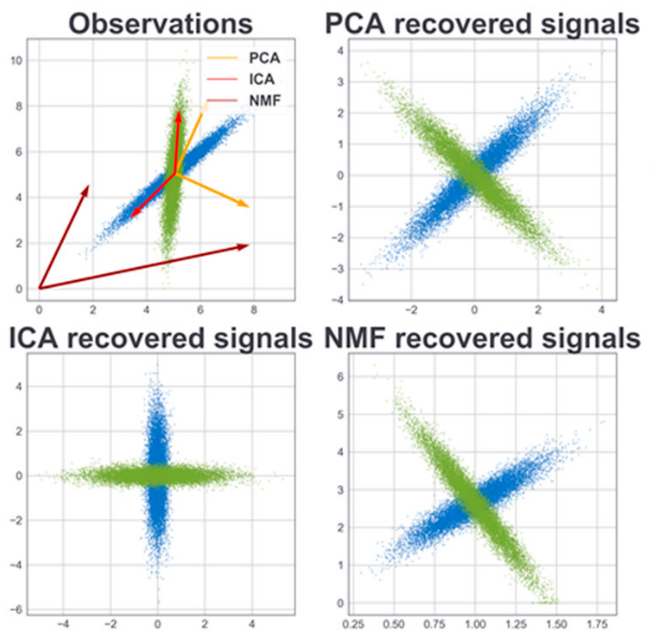
\includegraphics[scale=0.4]{Sompairac_ICA_NMF_PCA.png}
%\end{center}
%\caption{Illustrating the differing results of component extraction by PCA, ICA and NMF.  From \cite{Sompairac2019}}
%\label{fig-pca-ica-nmp-explanation}
%\end{figure}


Conventionally, expression arrays are oriented with genes (or transcripts) in rows, and samples (e.g. patients) in columns.   
A typical expression array might have in the order of tens of thousands of rows and hundreds of columns.  
MF methods reduces this large $m \times n$ (genes $\times$ samples) matrix into two smaller matrices.
In the general terminology of Stein-O'Brien \etal\ \cite{Stein-OBrien2018} these are the $m \times k$ \emph{pattern matrix} and the $k \times n$ \emph{amplitude matrix}.  $k$ is typically small of the order 10, and refers to the number of extracted \emph{factors} (or components); it is the rank of the factorization.
Since we are focussing on transriptomics, rather than pattern and amplitude we will use the terms \emph{metagenes} and \emph{metasamples} respectively, which are in common useage.  The symbol conventions for these matrices varies depending whether NMF, ICA or PCA is being discussed.   NMF generally uses $W$ and $H$ respectively while ICA generally uses $S$ and $A$.  PCA tends to be differently formulated, but $W$ and $T$ are often used.   The original matrix to be factorized is variously named $X$ or $V$.

In this work I wish to treat and discuss the three factorization methods in a unified way.  Thus, for the remainder of this dissertation the following notational conventions are adopted:
\begin{description}
\item[Expression matrix:] $X$ $(m \times n)$
\item[Metagene matrix:] $W$ $(m \times k)$
\item[Metasample matrix:] $H$ $(k \times n)$
\end{description}
where $N$ is the number of patients (or samples), $m$ is the number of genes and $K$ is the factorization rank, i.e. the number of components or factors.  Thus the factorization is written
\begin{equation}
X \approx W H
\end{equation}
Adding subscripts to indicate the row,column orientation of the matrices:
\begin{equation}
X_{m,n} \approx W_{m,k} H_{k,n}
\end{equation}
as illustrated in figure \ref{fig-matrix-factorization} (a).

\begin{figure}[htb!]
\def\M{2.2cm}
\def\N{1.3cm}
\def\K{0.3cm}
\def\fudge{-0.8mm}
\centering
\subfloat[Optimising independence of Meta\underline{genes}]{
\begin{tikzpicture}[node distance = 0.30cm, scale=1.1, every node/.style={scale=1.1}]
	\node (X) [draw, fill=green, minimum height=\M, minimum width=\N] {\large X};
	\node [right=of X] (eq) {\large $\approx$};
	\node [right=of eq] (S) [draw, fill=yellow, minimum width=\K, minimum height=\M] {\large W};
	\node [right=of S] (times) {\LARGE$\times$};
	\node [right=of times] (A) [draw, fill=cyan, minimum width=\N, minimum height=\K] {\large H};
	
	\node [below=\fudge of X] {\tiny{$n$ Samples}};
	\node [left=\fudge of X] {\rotatebox{90}{\tiny{$m$ Genes}}};
	\node [below=of X, text width=2cm, align=center] {\small Expression matrix};
	
	\node [below=\fudge of S] {\tiny{$k$ Metagenes}};
	\node [left=\fudge of S] {\rotatebox{90}{\tiny{$m$ Genes}}};
	\node [below=of S, text width=2cm, align=center] {\small Metagenes};
	
	\node [below=\fudge of A] {\tiny{$n$ Samples}};
	\node [left=\fudge of A] {\tiny{$k$}};
	\node [below=of A, text width=2.5cm, align=center] {\small Metasamples};
\end{tikzpicture}} 

\subfloat[Optimising independence of Meta\underline{samples}]{
\begin{tikzpicture}[node distance = 0.30cm, scale=1.1, every node/.style={scale=1.1}]
	\node (X) [draw, fill=green, minimum height=\N, minimum width=\M] {\large X};
	\node [right=of X] (eq) {\large $\approx$};
	\node [right=of eq] (S) [draw, fill=cyan, minimum width=\K, minimum height=\N]{\large W};
	\node [right=of S] (times) {\LARGE$\times$};
	\node [right=of times] (A) [draw, fill=yellow, minimum width=\M, minimum height=\K]{\large H};
	
	\node [below=\fudge of X] {\tiny{$m$ Genes}};
	\node [left=\fudge of X] {\rotatebox{90}{\tiny{$n$ Samples}}};
	\node [below=of X, text width=2cm, align=center] {\small Expression matrix};
	
	\node [below=\fudge of S] {\tiny{$k$ Metasamples}};
	\node [left=\fudge of S] {\rotatebox{90}{\tiny{$n$ Samples}}};
	\node [below=of S, text width=2.5cm, align=center] {\small Metasamples};
	
	\node [below=\fudge of A] {\tiny{$m$ Genes}};
	\node [left=\fudge of A] {\tiny{$k$}};
	\node [below=of A, text width=2cm, align=center] {\small Metagenes};
\end{tikzpicture}}
\caption{Two ways of configuring matrix factorization in the context of gene expression analysis.
In configuration (a) NMF and ICA will optimise the \emph{metagenes}, while in (b) the \emph{metasamples} are optimised. }
\label{fig-matrix-factorization}
\end{figure}

In the case of NMF and ICA, the $W$ and $H$ matrices cannot be trivially exchanged and transposed.  This is because the optimisations (sparsity and independence respectively) which define these algorithms are focussed on the $W$ matrix.  It is perfectly possible to apply these algorithms to gene expression analysis with exchanged and transposed meanings of $W$ and $H$, and this is illustrated in figure \ref{fig-matrix-factorization} (b).  In this case it is the properties of the \emph{metasamples} which are optimised.  Thus, the two forms are different in substance, not simply in notational convention.

There is substantial confusion and lack of clarity in the way that matrix factorization, particularly ICA, is applied in transcriptomics research.  
``Surprisingly, both ways of applying ICA to omics data are wide-spread, and sometimes it takes an effort to figure out in which way ICA was applied" \cite{Sompairac2019}, and ``Different protocols to apply ICA to transcriptomic data exist and currently no single standard approach has been defined. The main difference in the existing approaches consists in what is considered as source signal matrix in the decomposition" \cite{Cantini2019}.  
According to \cite{Cantini2019}, references \cite{Au-Yeung2014,Kairov2017,Kong2008,Lee2003},  optimise metagenes, while references \cite{Meng2016,Barillot2013} optimises metasamples.


\subsubsection{Determining the optimum number of factors}

The number of factors, or rank $k$, to extract is a key decision in any matrix factorization approach.  In this regard, PCA differs from ICA and NMF.  In PCA it is reasonable to extract all factors, setting $k=n$, the factors being ranked by the associated eigenvalue which also ranks the proportion of variance explained.   However, that approach is not valid for ICA and NMF, since differing sets of factors will be obtained for different $k$, and for a given choice of $k$ all factors are equally important -- they do not rank \cite{Stein-OBrien2018}.

The problem of determining the optimal $k$ for a given expression matrix is addressed  by Kairov \etal\ \cite{Kairov2017}, based on optimizing the \emph{stability} of the components over multiple algorithm initializations.

\subsubsection{Comparisons dimensionality reduction methods for gene expression analysis}
\label{sec-comparative-dimensionality-studies}

Recent work by Way \etal\ \cite{WayGregory2019} was aimed directly at answering the question of which dimensionality reduction method was best suited to gene expression data.  They considered PCA, ICA, NMF and also non-linear neural network methods -- directional autoencoders (DAE)  and variational autoencoders (VAE).  Briefly, these latter methods work by training a neural network to reconstruct an input signal while being forced through a network ``bottleneck''.   Their conclusion was that no single method was optimal, but best performance -- judged by capturing the most biological pathway-associated features -- was achieved by taking the extracted latent dimensions of all the methods, an approach they call the ``BioBombe''.

Meng \etal\ \cite{Meng2016} extensively review dimensionality reduction methods applied to multi-omic datasets.   PCA, ICA and NMF are discussed, but the main focus is on less well known algorithms applicable to multiple datasets, including multiple coinertia analysis and consensus PCA.  The essential purpose of these methods is to transform diverse datasets -- transcriptomics, genomics and metabolomics  -- into a crommon and manageable representation space.

The question of reproducibility across datasets of matrix factorization methods is considered by Cantini \etal. \cite{Cantini2019}.  They experiment with several MF methods applied to a total of 26 cancer transcriptomic datasets (including ovarian).  They conclude the best approach to be ICA, stabilized by the use of Reciprocally Best Hit graphs; in essence requiring reciprocal identification of metagenes between at least two datasets.

\subsection{Research gaps and questions}
Considering the foregoing review of the literature, there has clearly been much work by large teams of researchers directed at understanding the gene expression patterns in HGSOC, as one would expect given its clinical importance.  
Dimensionality reduction is a huge and active field -- the bread-and-butter of machine learning research. 
As we have seen, conclusions both on the underlying biology and the optimal methodology are far from consistent, however.   Some approaches -- such as the BioBombe reviewed above -- are complex with results likely to be difficult to reproduce.   

Robustness of research results is of course fundamental.  MF methods offer a means of \emph{unsupervised} learning on transcriptomic datasets to identify key genes active in a disease process.  Would two teams working with identical data and using similar MF methods obtain similar metagenes and so arrive at the same biological conclusions?   The \emph{stability} of MF methods is well considered by many authors, although this has typically been focussed on stability of the underlying algorithm -- NMF and ICA are stochastic in nature, sensitive to initial conditions.   Much less considered is stability in the presence of \emph{sampling error} which inevitably exists particularly in small datasets.

These and wider considerations suggest the following research questions.

\begin{enumerate}
\item What underlying biological processes are at play in HGSOC as seen through the patterns of gene expression?  Do these confirm published results?
\item How do the patterns of gene expression uncovered relate to genome level features, such as those marking genome instability?
\item Do MF methods yield factors which are predictive of patient survival?
\item How should MF methods be applied to achieve robust results on datasets of limited size?
\item Does MF detect and remove technical batch effects?
\item Which MF method is best suited to transcripomics analysis?
\end{enumerate}


%%%%%%%%%%%%%%% METHODOLOGY %%%%%%%%%%%%%%%%%

\section{Methodology}

\subsection{Outline}

Our overall approach is to use \emph{unsupervised} machine learning methods to represent gene expression data in a small number of features, then to study whether these features correlate with clinical and biological variables.  Unsupervised methods have the advantage of being applicable to large datasets for which metadata (e.g. clinical information) is not available.  Results can then be transferred to smaller datasets which do have metadata.   This is appropriate in our case, since of the two datasets available (described below), one (TCGA) has relatively large n but little available metadata, while the other (AOCS) is much smaller but has more useful metadata of genomic features.   This motivates an approach of unsupervised learning on the TCGA dataset which is then transferred to the AOCS dataset for evaluation.

\subsubsection{Datasets}
Two gene expression datasets were made available for this work (N refers to number of patients, m refers to number of protein coding genes).
\begin{enumerate}
\item The Cancer Genome Atlas (TCGA) derived, N=374 patiens, m=19,601 genes, with metadata on survival
\item Australian Ovarian Cancer Study (AOCS) \cite{Patch2015}, N=80, m=19,730, with metadata on survival, cellularity and additional genomic features. Several of the studies reviewed earlier also use data from the Australian Ovarian Cancer Study (AOCS): \cite{Patch2015,Ewing2020,Cuello2018,Au-Yeung2014}.
\end{enumerate}

Expression data for the AOCS and TCGA datasets was received for this project in spreadsheet format, having been derived from the RNA-Seq data with normalization by variance stabilizing transformation applied.  The RNA-Seq data is publicaly available, downloadable from  the \href{https://dcc.icgc.org/pcawg}{Pan-cancer Analysis of Whole Genomes (PCAWG) data portal} for AOCS, and from the \href{https://portal.gdc.cancer.gov/}{Genomic Data Commonas (GDC) data portal} for TCGA.  The provenance and processing of these datasets is described in \cite{Ewing2020}.


\subsubsection{Methods}
An overview of the methodology adopted in this work is shown in figure \ref{fig-method-overview}, consisting of:

\begin{figure}[htb!]
\begin{center}
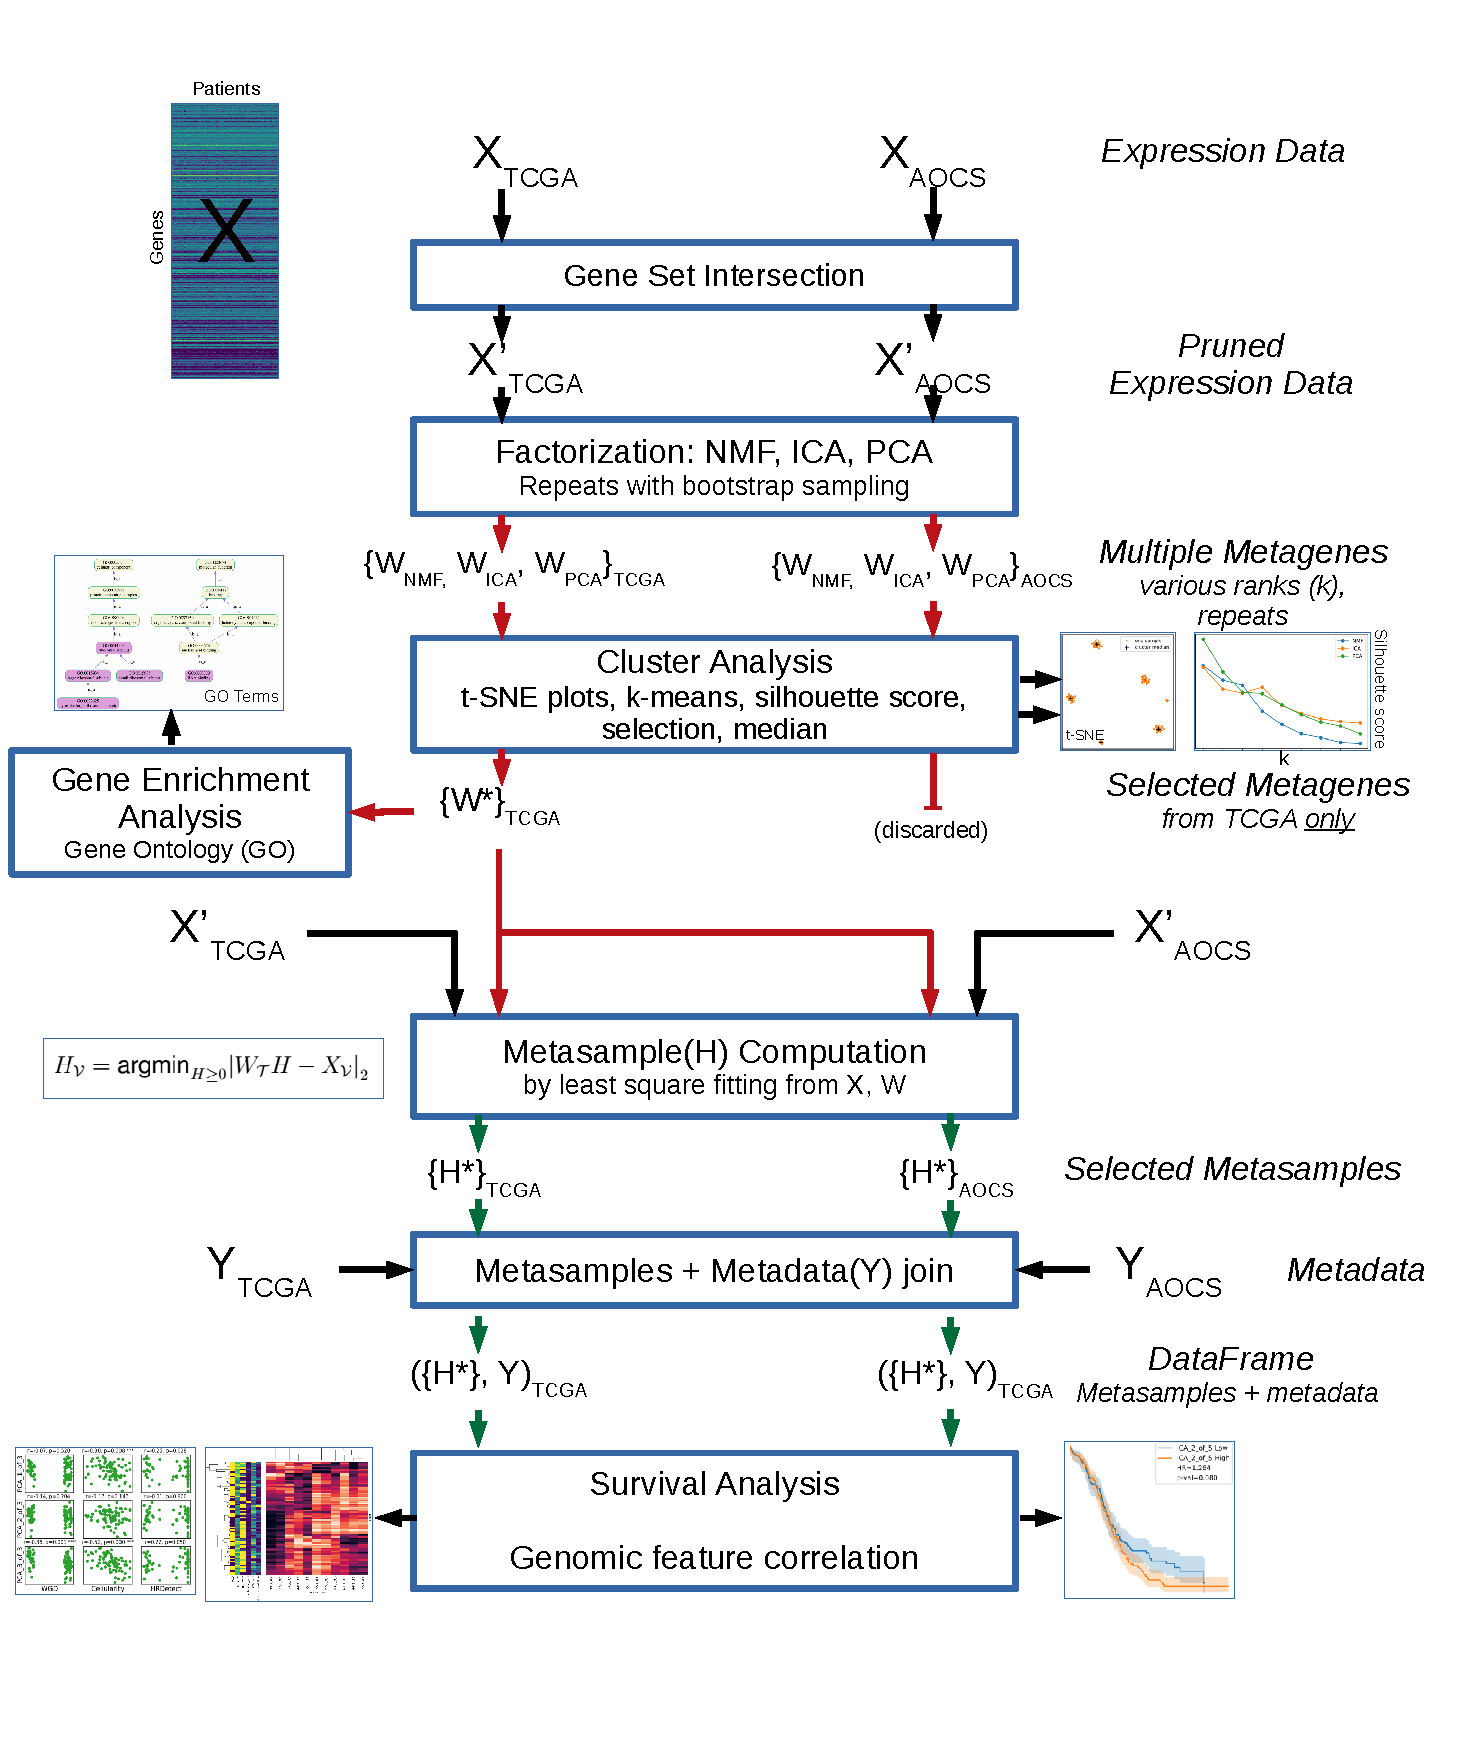
\includegraphics[scale=0.6]{methodlology_overview.pdf}
\end{center}
\caption{Overview of methodology as information flow.  The diagramatic convention here is that at each stage, both datasets -- TCGA and AOCS -- are processed separately by the given algorithm.  The exception is Gene Set Intersection, which involves interaction between the datasets.  (The investigation of batch effects on the combined dataset is not shown in this diagram to avoid over complexity). }
\label{fig-method-overview}
\end{figure}

\begin{enumerate}
\item
Identification of a consistent gene set between the TCGA and AOCS datasets.
\item
Unsupervised metagene extraction by matrix factorization methods : NMF, ICA and PCA.
\item
Metagene selection for robustness by k-means clustering of bootstrap resampled factorizations evaluated by silhouette score, based on the TCGA dataset.
\item
Investigation of biological significance of extracted metagenes by gene enrichment analysis (GEA) against the Gene Ontology (GO).
\item
Computation by least squares optimisation of metasamples associated with each TCGA derived metagene against TCGA and AOCS datasets.
\item
Alignment of available metadata with computed metasamples, for TCGA and AOCS.
\item 
Survival analysis on TCGA and AOCS to investigate relationships between metasamples and patient survival.
\item
Scatter plots and heat maps to investigate the relationships between metasamples and genomic features available for the AOCS dataset.
\item
Investigation of batch effects by repeating the above analysis pipeline on the \emph{combined} AOCS / TCGA dataset (N=80+273=353).

\end{enumerate}

These steps are detailed in the following main sections.

\FloatBarrier

\subsubsection{Tools}
\begin{itemize}
\itemsep -0.5em 
\item DELL XPS 13, 16GB RAM, running Linux Mint version v19.
\item Python v3.6.8
\item PyCharm Integrated Development Environment, v2020.1.3
\item Numpy for high performance matrix manipulation, v1.18.15
\item Pandas for data frame handing, v1.0.5
\item Matplotlib and Seaborn for general plotting, v3.2.2 and v0.10.1
\item SciPy for least-square solutions and statistical tests, v1.5.0
\item Scikit-learn for matrix factorization and k-means clustering, v0.23.1
\item GOATOOLS package for GEA against GO, v1.0.6
\item Lifelines package for survival analysis, v0.24.16.
\item Github for source control.
\end{itemize}

\subsection{Syncrhonisation of gene sets accross AOCS and TCGA}
\label{sec:gene-set-intersection}

In order to allow factorizations found in the TCGA dataset to be applied to the AOCS dataset it is necessary (or at least convenient) to synchronize the set of genes over which the expression matrices are defined.   As provided to this project, the TCGA and AOCS datasets cover 19,610 and 19,730 protein coding genes respectively, 19,566 of which are common to both (according to ENSG encodings).  Thus, both datasets were pruned to the 19,566 intersection set and ordered consistently.

\subsection{Matrix factorization computation}
One of the aims of this work is to compare the efficacy of three methods of dimensionality reduction -- NMF, ICA and PCA -- as explained in the introduction.     
Some of the key algorithm hyper parameters of each method were investigated and tuned with respect to reconstruction accuracy, specifically the root-mean square (RMS) difference between $X$ and $W H$. The following parameters were explored in each case:
\begin{description}
\item[NMF:] Parameters {\tt max\_iter} (algorithm iterations) and {\tt tol} (tolerance of convergence) were optimised for good accuracy and acceptable execution time.   
{\tt max\_iter} = 5000 and {\tt tol} = 0.01 was used.
Other parameters of interest are {\tt alpha} (multiplier for regulation term) and {\tt l1\_ratio} (multiplier for L1 regularization, when {\tt alpha} $> 0$).  L1 regularization  favours elements being precisely zero, whereas L2 regularization will encourage them to be small.  These parameters have not been explored in this project, and the default {\tt alpha = 0} (no regularization) was used.
\item[ICA:]  Parameters {\tt max\_iter} and {\tt tol} were investigated as for NMF above. 
{\tt max\_iter} = 5000 and {\tt tol} = $10^{-5}$ was used.
Additionally, options for the entropy function which forms the basis of the optimiziation were investigated.
\item[PCA:] This is in principle a deterministic algorithm based on eigenvector decomposition.  However, {\tt sklearn.decomposition.PCA} uses a more efficient 'randomized' algorithm when the given matrix is larger than 500 in both dimensions.  Thus in our use case PCA is seen to have (slightly) stochastic behaviour.
\end{description}

\subsection{Metagene extraction by cluster coherence under bootstrap resampling}
\label{sec-metagene-selection}
Deciding on the number of components (factors, metagenes) to extract -- that is the factorization rank -- is key.  Taking more components results in more accurate representation of the observed expression matrix and provides more avenues to explore the underlying biology.  However, it is important that the metagenes are \emph{stable}, that is that they have reliable meaning when transfered to other datasets.   There are two sources of variation or instability to consider.

Firstly, NMF and ICA are inherently stochastic algorithms, sensitive to their starting state, so repeated runs give different results.

A second and more fundamental source of variation of relevance to all three factorization methods is \emph{sampling error}.   Our factorizations are based on a small ($N=80$ or $N=374$) sample of patients drawn from the population of HGSOC patients; our particular datasets are just two examples of many different ``draws" which could have been made from that population.

\emph{Bootstrap sampling} (also know as \emph{Monte Carlo} simulation) is a common method of empirically propagating the consequence of sampling error when the distribution or processing operations are difficult to model mathematically.   This is implemented by performing factorizations multiple times, at each iterations choosing N samples from the N available \emph{with replacement}.   For this work 50 repeats were performed, being a compromise between achieving an adequate simulation without overly burdensome computation time.  The process is described below and summarised as pseudocode in figure \ref{fig-clustering-psuedocode}.  

A complication arises in the computation of ICA and PCA factorizations, in that essentially the same factor can arise as $w$ or $-w$ -- i.e. $180^\circ$ rotated vectors. These would appear as separate clusters in repeated sampling, and confound attempts to collect and aggregate.  The solution adopted here is to normalise each factor by requiring that the most extreme element -- i.e. having the greatest absolute value -- is positive, the whole factor being negated if this is not the case.  This is arguably over simplistic, but seems to be effective in practice.

Each of the three factorizer methods was evaluated for rank $k$ between 2 and 10.  In each case, 50 iterations of factorization are performed on bootstrap samples, generating $50 k$ instances of 19,566 dimensioned metagenes.  Two dimensional t-SNE plots were generated for visualization purposes.   If sampling and algorithm initialisation error are modest then we expect to see $k$ tight clusters of points.   To avoid lengthy computation in the t-SNE clustering, the metagenes were first reduced to $r=20$ dimensions by PCA; brief experiments showed that this reduction had negligible effect on the t-SNE visualisation providing $r \geq 10$.   

In order to obtain median estimates of the $k$ metagenes from the $50 k$ which were generated, k-means clustering was performed in the PCA reduced ($r=20$ dimension) space, delivering $k$ sets of points.  These were referenced back to the original 19,566 dimensioned metagenes and the per-dimension median calculated.  These $k$ median metagenes were saved to a file named for the specific factorizer and rank $k$.  

The k-means clustering further allowed for a quantitative assessment of cluster coherence for the particular choice of factorizer and rank, via the \emph{silhouette score} (see \cite{Wikipedia}).  In brief, this is a measure of how close (by Euclidean distance) each point in a cluster is to other points in the cluster versus points in \emph{other} clusters.  
The score is in the range -1 to +1, with 0 implying random scatter and 1 implying all points of a cluster perfectly overlay.

The t-SNE plots and silhouette scores were assessed visually to decide, for each of the three factorizers, the highest rank with good cluster coherence.  The median points of those clusters then formed the metagenes to take forward to gene enrichment, survival and genomic feature correlation analysis.   
Note that the t-SNE plots are used only for visualisation; they are not involved in the computation of median metagenes or silhouette score.

Initial investigation on the N=80 AOCS dataset showed very poor cluster coherence, even for k=2.   Thus, it was decided to compute and select metagenes only from the N=374 TCGA dataset.   
The selection rationale is set out in the results section, but it is convenient to state here that the following ranks were selected:
$K_{\mbox{\tiny NMF}} = 3, K_{\mbox{\tiny ICA}} = 5, K_{\mbox{\tiny PCA}} =3$.  Thus, there were $3 + 5 + 3 = 11$ metagenes taken forward for follow-on analysis.

A point to be aware of is that because PCA metagenes are treated the same as NMF and ICA metagenes, being extracted by the same clustering approach, the \emph{ordering} of PCA components is not necessarily maintained.   Thus, component 'PCA-1' is not necessarily the first PCA component  in the usual sense -- i.e. the component capturing greatest variance.  This could be fixed but would require special case code.

\begin{figure}[htb!]
\begin{center}
\begin{Verbatim}[baselinestretch=1, frame=single, rulecolor=\color{blue}, label=Metagene Stability Assessment, fontfamily=courier, fontsize=\small]

 for factorizer in NMF, ICA, PCA:
    for k in 2..10:
       Ws = []
       for j in 1..50:
          X = bootstrap sample N from N with replacement
          W, H = factorizer(X, rank=k, seed=j)
          append W to Ws
   	     
       # Ws is a list of 50*k metagenes, each of length 19,566
       # Pragmatically reduce metagenes to 20 dimensions by PCA
   	  
       Ws_reduced = PCA(Ws, rank=20)
       plot t-SNE(Ws_reduced)
       clustering = k-means clustering(Ws_reduced, n_clusters=k)
       score[factorizer, k] = silhouette score(clustering)	  
       median_metagenes = calculate medians for k clusters of metagenes
       save median_metagenes to file by factorizer and k
    plot score vs for factorizer k
      
\end{Verbatim}
\end{center}
\caption{Pseudocode for generating median metagenes and assessing their stability to random algorithm initialization and sampling error.}
\label{fig-clustering-psuedocode}
\end{figure}

\subsection{Determining metagene similarity by Jaccard index}

It is pertinent to ask ``how similar are the 11 metagenes which emerge from the foregoing factorization and cluster analysis?''.  We expect those coming from a single factorization method to be distinct by construction.  But perhaps ICA and PCA identified similar components.  Similarity with NMF derived components is possible but less likely due to the positivity constraint.  A possible approach to measuring similarity might be to treat the components as vectors and determine the angle between them, via the scalar or ``dot'' product.  But in such a high dimension space (19,566) any pair of vectors will be very close to $90^\circ$.

An alternative is to consider the intersection of the gene sets which each metagene highlights.  In the GEA which follows, candidate genes will be identified for each meatagene.  A standard measure of set similarity is the Jaccard index, (or similarity), defined on a pair of sets as:

\[
   \mbox{Jaccard}(A, B) = \frac{A \cap B}{A \cup B}.
\]
The measure lies between 0 (no similarity) and 1 (identical), and is symmetric.  Jaccard similarity was thus calculated for all pairs of the 11 genes sets and visualised as a square heatmap.
	   	  
\subsection{Gene enrichment analysis (GEA)}
\label{sec-gea}
The metagenes extracted by the above described factorization and clustering process provide valuable information into which genes vary in expression in the study samples; thus in our case, which genes are influential in the dominant expression signal in HGSOC.  
In order to gain insights into what biological processes are involved, GEA against the Gene Ontology (GO) was carried out for each of the 11 metagenes individually.

The essence of GEA is to compare a candidate set of genes with many functional gene sets, asking the question ``are there significantly more (or less, i.e. depletion) intersecting genes than would be expected for the same number of genes being drawn at random (without replacement) from the total population of genes in the study. 

For each metagene, the candidate gene set was determined as those genes having weights outwith three standard deviations of the mean.   This set was analysed using the Python GOATOOLS package \cite{Klopfenstein2018}.   

The gene ontology was downloaded from \url{http://purl.obolibrary.org/obo/go/go-basic.obo}.  ({\tt Purl.org} is a resource for managing permanent URLs; {\tt obo} refers to the Open Biological and Biomedical Ontology (OBO)).  
Annotations linking human genes to GO concepts was downloaded from the GO website, specifically \url{http://geneontology.org/gene-associations/goa_human.gaf.gaf}.   
The gene population was defined as the common 19,566 protein coding genes (see section \ref{sec:gene-set-intersection}) against which the metagenes were computed.  

Uncorrected p-value threshold was set to 0.01.
Multiple hypothesis significance testing used the false discovery rate (FDR) method of Bengamini and Hochberg, the FDR threshold being set to 0.01.  This is more stringent than the 0.05 value which is commonly used, and was chosen since multiple metagenes are being analysed, implying multiple hypothesis testing over and above that which is accounted for by FDR filtering within a single GEA run.  (Arguably, $0.05 / 11 \approx 0.005$ should have been used).

\begin{figure}[htb!]
\begin{center}
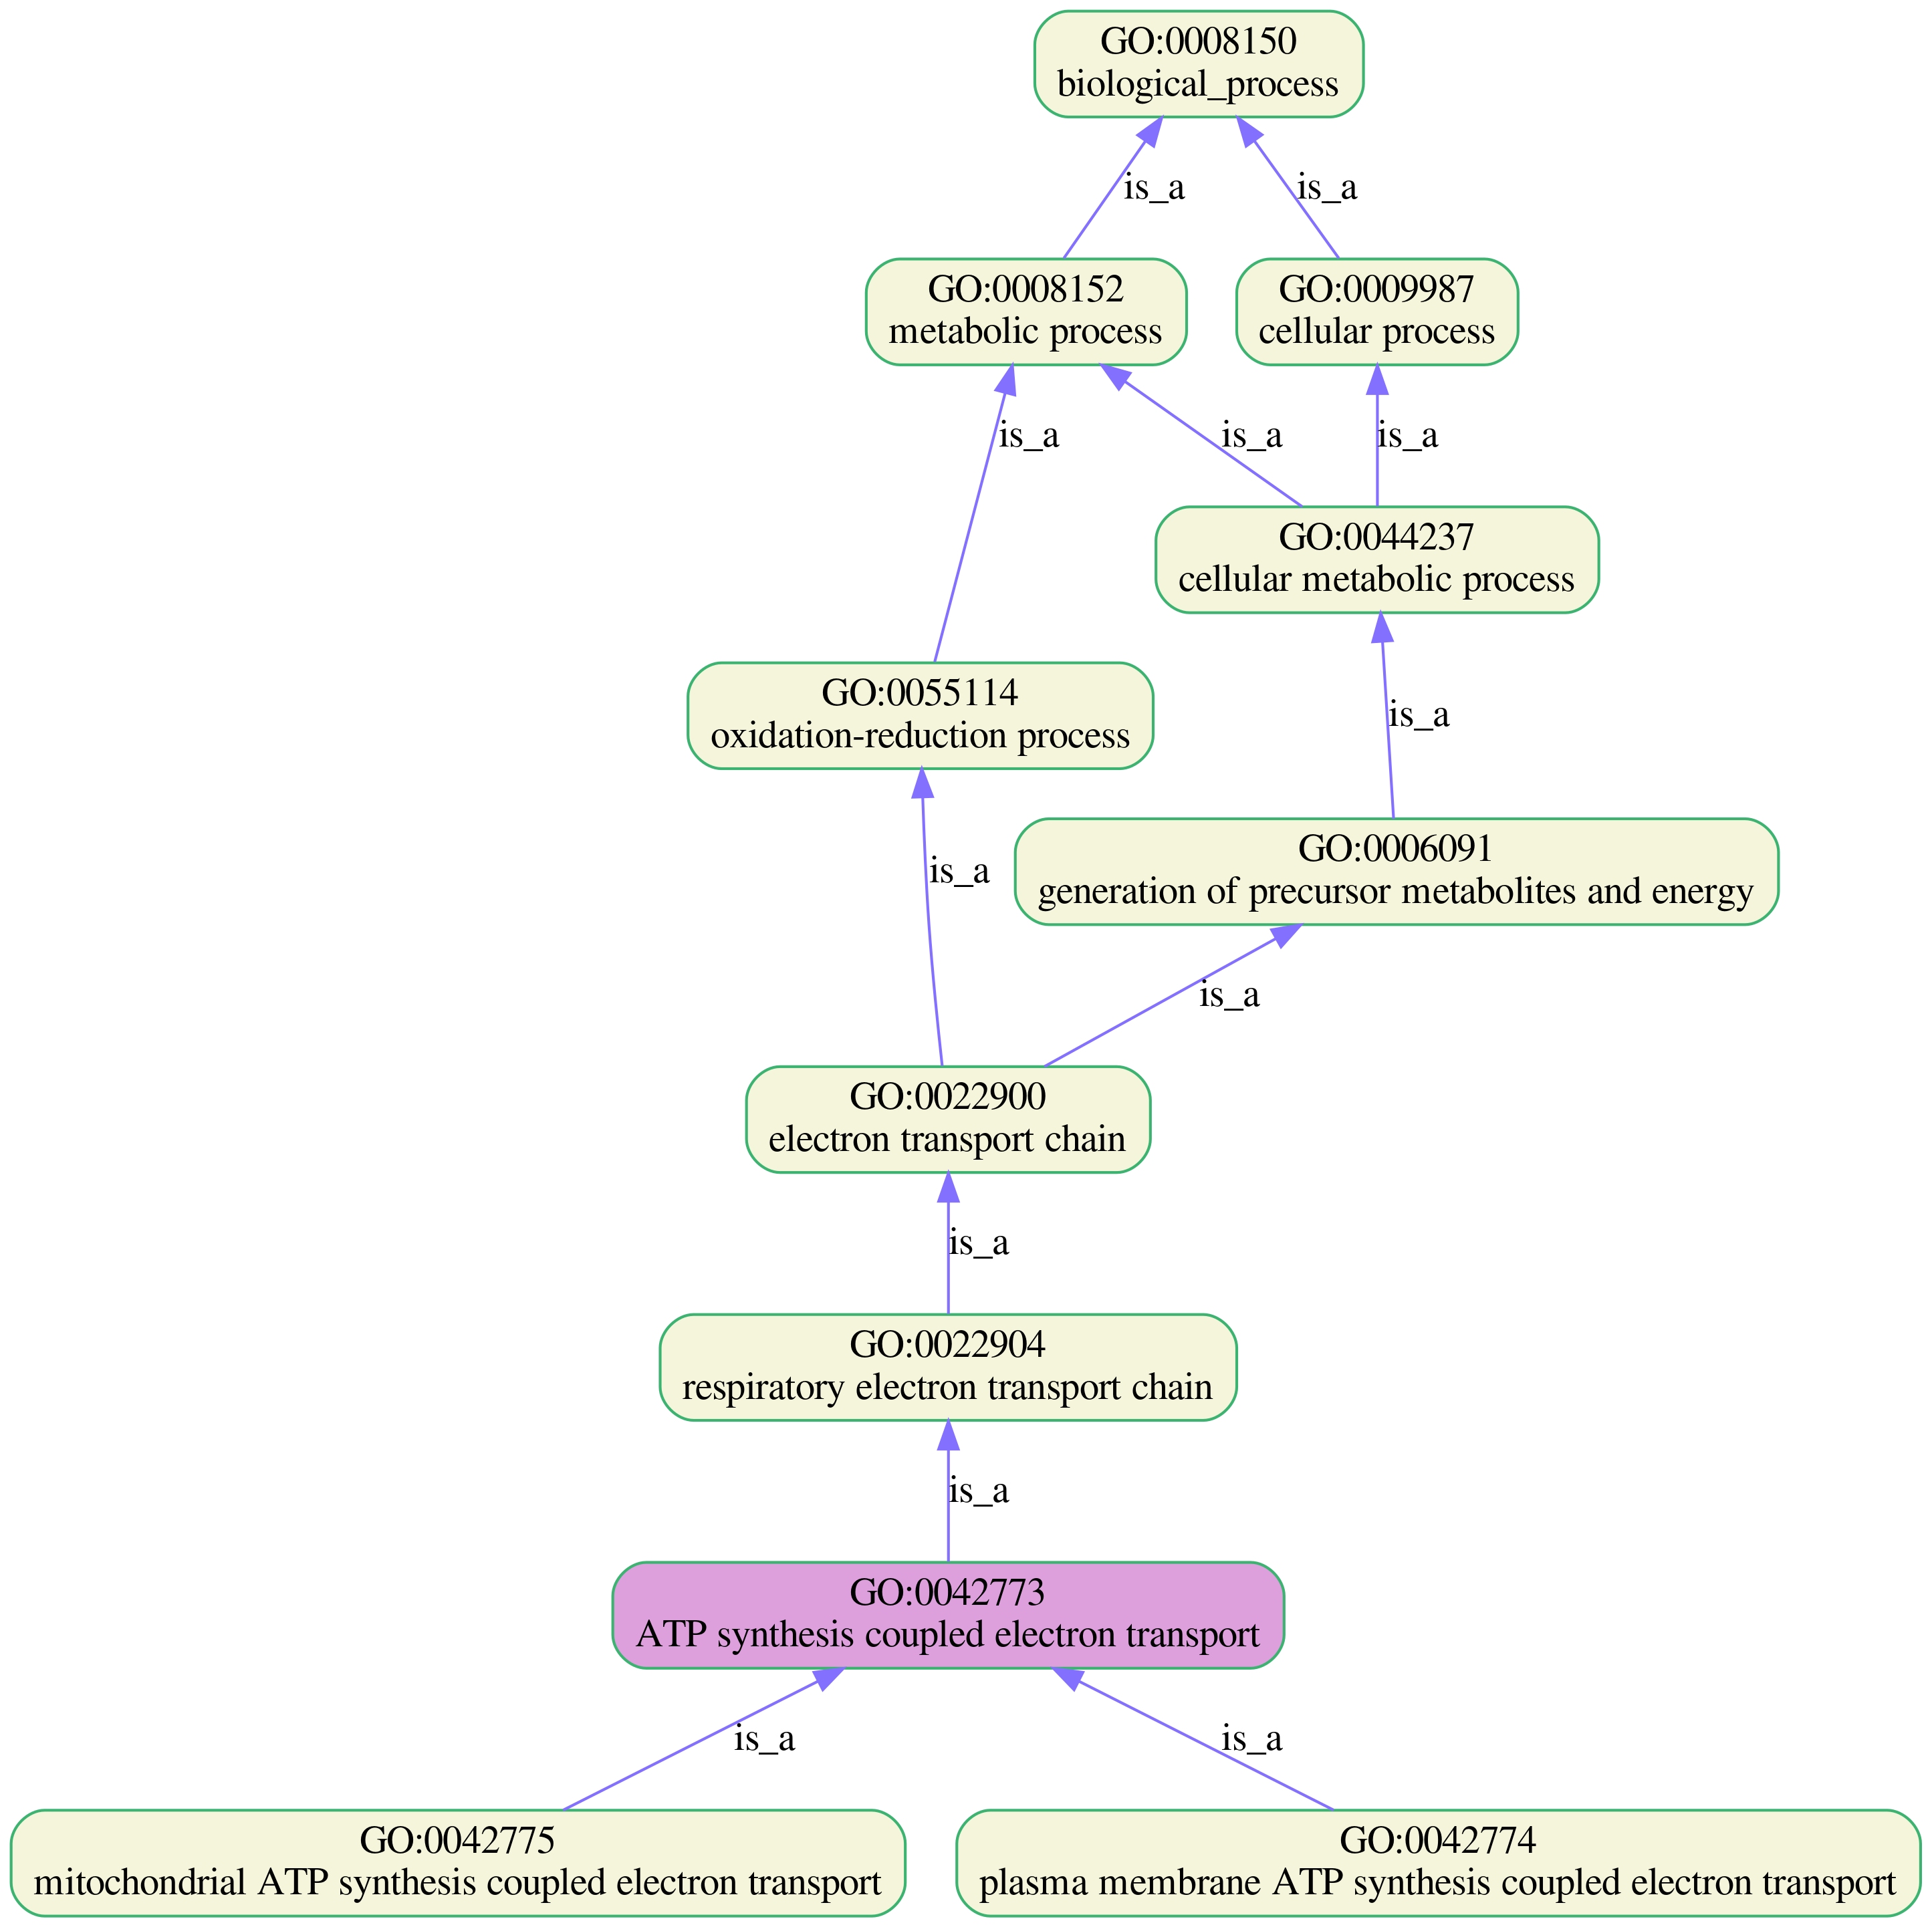
\includegraphics[scale=0.13]{GO_0042773_lineage.png}
\caption{Example of a small section of the Gene Ontology (GO), focussed GO:0042773 (in purple), showing parents and children of the term.   Generated by GOATOOLS.}
\label{fig-eg_go_graphic}
\end{center}
\end{figure}

The result of this analysis, per metagene, is a list of enriched (or depleted, however no depleted terms were found) GO terms, each with an associated list of involved genes and a FDR significance level.   This list can be inspected directly for insights, but that misses the point of the GO, which is to organise the terms hierarchically by `is a' relationships.   Thus, the enriched terms were rendered graphically to show them in the context of their parent terms; an example is shown in figure \ref{fig-eg_go_graphic}


\subsection{Transfer of learned metagenes to a novel dataset}
\label{sec-transfer-to-novel}

\newcommand{\trainset}{\mathcal{T}}
\newcommand{\validset}{\mathcal{V}}

It is fundamental to our approach that \emph{metagenes} determined on the basis of one (large but metadata poor) dataset can be used to generate \emph{metasamples} for a different (small but metadata rich) dataset.   In the exposition below we refer to these as the \emph{training} and \emph{validation} cohorts respectively.
Rank $k$ matrix factorization on the training dataset $\trainset$ (e.g. TCGA) results in:
\begin{equation}
 X_\trainset \approx W_\trainset H_\trainset
\end{equation}
where $X_\trainset$ is the expression matrix of shape $(m_\trainset, n_\trainset)$, with $m_\trainset$ the number genes and $n_\trainset$ the number of patients. $W_\trainset$ is the metagene matrix of shape $(m_\trainset, k)$ and $H_\trainset$ is the metasamples matrix of shape $(k, n_\trainset)$.

We wish to apply the factorization learned on $\trainset$ to a novel dataset $\validset$ (specifically the AOCS dataset) of shape $(m_\validset, n_\validset)$. 
Importantly, $n_\validset = 1$ reflects the application of these methods to a single patient in a clinical setting.  To apply the learned factorization we need to find $H_\validset$ as in the factorization
\begin{equation}
	X_\validset \approx W_\validset H_\validset
\end{equation}
In both the experimental and clinical situation we are given $X_\validset$ but not $W_\validset$ and require to find $H_\validset$. 
We \emph{cannot} simply perform the matrix factorization on dataset $\validset$ since $n_\validset$ may be small, or even a single patient.   
However, if patients in datasets $\trainset$ and $\validset$ are drawn from the same population (ovarian cancer patients), then $X_\trainset$ and $X_\validset$ can be expected to have similar distributions w.r.t to their columns, and thus $W_\trainset$ and $W_\validset$ can be expected to be equivalent within sampling error.  
This only makes sense if the two expression matrices $X_\trainset$ and $X_\validset$ are defined over the \emph{same set of genes}, so that $m_\trainset = m_\validset = m$, in which case $W_\trainset$ and $W_\validset$ have the same shape of $(m, k)$.   

We thus need to solve for $H_\validset$ in
\begin{equation}
	X_\validset  \approx  W_\trainset H_\validset \label{eq_Xv_WtHv}
\end{equation}

This can be solved by the method of least squares.  In the case that the original factorization was by NMF, we use non-negative least square regression (NNLS):
\begin{equation}
	H_\validset = \mbox{argmin}_{H\geq 0}{\lvert W_\trainset H - X_\validset \rvert}_2
	\label{eq_Hv_WdtXv}
\end{equation}
where ${\lvert \mathbf{\cdot} \rvert}_2$ indicates Euclidean distance or L2-norm.
The function {\tt scipy.optimize.nnls} is used.
For ICA and PCA we use ordinary least square regression, formulated as above but dropping the $H\geq 0$ constraint, using {\tt scipy.linalg.lstsq}.

%An internal check on the validity of the statistical assumptions can be made my substituting  $H_\validset$ from (\ref{eq_Hv_WdtXv}) into (\ref{eq_Xv_WtHv}) and assessing the accuracy of the approximation by RMS difference.

The end result of the analysis is the $H_\validset$ matrix of shape $(k, n_\validset)$, thus delivering for each dataset in our $\validset$ a feature vector -- or metasample -- of length $k$. 

Since in this work the efficacy of three factorization methods are being studied (NMF, ICA and PCA), three different $H$ matrices are taken forward, each having ranks as for the associated metagenes (3, 5 and 3 respectively).

\subsection{Reconciling computed metasamples and metadata}
\label{sec-reconciling-metasamples-metadata}

To carry out patient level analysis -- survival analysis, heatmaps and genome feature correlation -- as described in the following sections, it is necessary to compile tables (Pandas DataFrames) which bring together per-patient metasamples relating to each of the selected metagenes, with associated metadata -- such as cellularity and survival information.   The metagenes always derive from the TCGA dataset (because of its larger size as explained in section \ref{sec-metagene-selection}), but we wish to apply these metagenes as metasamples to the expression data and associated metadata of either the TCGA or AOCS datasets.   
The mathematics of transferring metagenes across datasets has been described above.  Care is required to ensure that expression matrices are aligned correctly with metagenes with respect to their genes, and that metadata is aligned correctly with metasamples with respect to patient identifiers.
Note that the same transferring approach is taken when metasamples are required for TCGA, even though we could in that case obtain the $H$ matrix directly from the factorization.


\subsection{Survival analysis}
\label{sec-survival-analysis}

Survival analysis was performed to investigate whether the metasamples derived from the selected metagenes correlate with patient survival.  Overall  survival (OS) data is available for both the TCGA and AOCS datsets.  Additionally, progression free survival (PFS) data is available for AOCS.   As described above,  metagenes were obtained by factorization on the TCGA dataset only.  Application to TCGA (for OS) thus represents an in-sample test, while application to AOCS (for OS and PFS) is a more exacting out-of-sample test. There are thus three analyses to consider: 
1) TCGA$\rightarrow$TCGA (OS) meaning TCGA derived metagenes are tested for OS on the TCGA dataset, 2) TCGA$\rightarrow$AOCS (OS) meaning TCGA derived metagenes are tested for OS on the AOCS dataset, and 3) TCGA$\rightarrow$AOCS (PFS)... as 2) but for PFS. 

Analysis was performed using the Python {\tt Lifelines} package \cite{Davidson-Pilon2020}.  
%Metasamples ($H$ matrices) were calculated from the metagenes and expression matrix as explained in section \ref{sec-transfer-to-novel} below.  
Metasample values were binarized to 0, 1 by thresholding at the median value.   Kaplan-Meier plots were made in respect of derived metasample for each of the three analyses -- making $11 \times 3$ plots each with two survival curves with 95\% confidence intervals.  A hazard ratio (HR)
was calculated for each analysis by fitting Cox's proportional hazards model with p-value relating to the hypothesis that HR is significantly different to 1.0.


\subsection{Investigating correlation between metasamples and genomic features}
\label{sec-genomic-features}

For the AOCS dataset (only) per-patient high-level genomic features were available as follows:
\begin{description}
\item[WGD]: Whole genome doubling -- a marker of genome instability, a binary feature.
\item[Cellularity]: proportion of cells belonging to the tumour (as opposed to surrounding normal tissue).
\item[HR Detect]: A predictor of homologous repair deficiency based on established mutational features \cite{Ewing2020}.
\item[Mutational Load]: A measure of the total number of mutations present in the tumour genome.
\item[CNV Load]: Copy-number variation, i.e. deviation from the normal diploid cell compliment.
\item[SV Load]: Structural variation, a measure of the degree of chromosomal rearrangements such as translocations and inversions.
\end{description}

Scatter plots were generated between each metasample and each genomic features -- a grid of $11 \times 6 = 66$ plots in all.  These were based on the reconciled metasamples and metadata as described in section \ref{sec-reconciling-metasamples-metadata}.  Pearson's correlation coefficients ($r$) and associated p-values (i.e. the probability that $r$ does not differ from zero) were calculated.   However, since WGD is a binary feature, the more appropriate Point-Biserial correlation (see \cite{Wikipediab}) was used in that case.  A p-value significance threshold of 0.01 was chosen, although with 66 hypotheses being tested, this does risk false discovery.

As an alternative visualisation of the relationship between metasamples and genomic features, and to see the relationship between metasamples themselves, a clustered heatmaps was generated using the \href{https://seaborn.pydata.org/generated/seaborn.clustermap.html}{Seaborn {\tt clustermap()}} function based on the same underlying data as above.  

\subsection{Investigating batch effects by analysis of a combined dataset}

It has been claimed (e.g. \cite{Stein-OBrien2018,Renard2016}) that matrix factorization methods are an effective means of identifying and removing batch effects.  To verify this, the TCGA and AOCS datasets (after gene set intersection), were horizontally concatenated producing an $N=80+374=454$ patient dataset with a known batch artefact.  All of the previously described analyses were repeated for this combined dataset (however, survival analysis is not shown).  Ideally, the factorization rank selected for each method should be reconsidered, since the larger dataset could justify extracting more components.  For simplicity this was not done however, the previously selected $k = 3,5,3$ for NMF, ICA and PCA respectively being maintained.   Note however that we should not expect the extracted metagenes and derived metasamples to be equivalent. Genomic feature correlation w.r.t these newly extracted components was performed using the AOCS datasets.  These results were inspected for evidence of some metasamples aligning with technical batch effects while others align with biological processes.

\subsection{Codebase and plotting conventions}

The described methodology was implemented in Python.
%except for the KEGG GEA which was implemented in R.
All code is available in a github repository: \url{https://github.com/ipoole/HgsocTromics}.  Good software engineering practice has been followed, with an object-oriented design, frequent commits and unit testing.  A base class is used to present a uniform interface for the three factorization methods.  Intermediate results are cached to file with lazy computation for efficient working without imposing evaluation order dependency.  Unit tests are based on tiny expression matrices, just 100 genes by 10 patients, thus the whole test suite of over 65 tests executes in around 45 seconds.   The fully automated (except for rank selection) analysis pipeline takes approximately three hours from scratch, the majority of that time being taken for the repeated factorizations over the range of considered ranks.  The total codebase is approximately 2,900 lines of Python.  

All plots are generated in vector graphics pdf format to ensure smooth scaling to any resolution.  A consistent colour scheme of \textcolor{blue}{blue}, \textcolor{orange}{orange} and \textcolor{olive}{green} is used for plots relating to NMF, ICA and PCA respectively.  In figures metagenes / metasamples are consistently referred to by, for example, ``NMF-2-of-3" -- meaning the 2nd component of the rank $k=3$ NMF factorization.  In text this is shortened to ``NMF-2'' where the rank is understood.


%%%%%%%%%%% RESULTS %%%%%%%%%%%%%
\clearpage

\section{Results}


% \subsection{Investigation of optimal parameters}
\subsection{Consideration of sampling error is crucial to finding robust metagene signals}

From figure \ref{fig-AOCS-ica-fixed-vs-bootstrap} it can be seen that with sampling error excluded (top), clusters appear reasonably coherent, but when sampling error is modelled by bootstrap sampling then  the factorizations become much less stable.  This demonstrates that \emph{sampling} error is far greater than errors due to algorithm initialisation when the dataset is small (N=80), making metagene extraction unreliable.   Figure  \ref{fig-TCGA-ica-fixed-vs-bootstrap} makes the same comparison for the larger N=374 TCGA dataset, in which it can be seen that the impact of sampling error is not so severe.  For brevity only results for ICA are shown here; similar result for NMF and PCA can be found in the appendix, figures \ref{fig-AOCS-nmf-fixed-vs-bootstrap} and \ref{fig-AOCS-pca-fixed-vs-bootstrap}.

For this reason it is was decided to perform all metagene extraction on the larger TCGA dataset, in the expectation that the obtained metagenes will be more robust and likely to better generalise to other datasets.

\def\S{0.4}
\begin{figure}[htb!]
\begin{center}
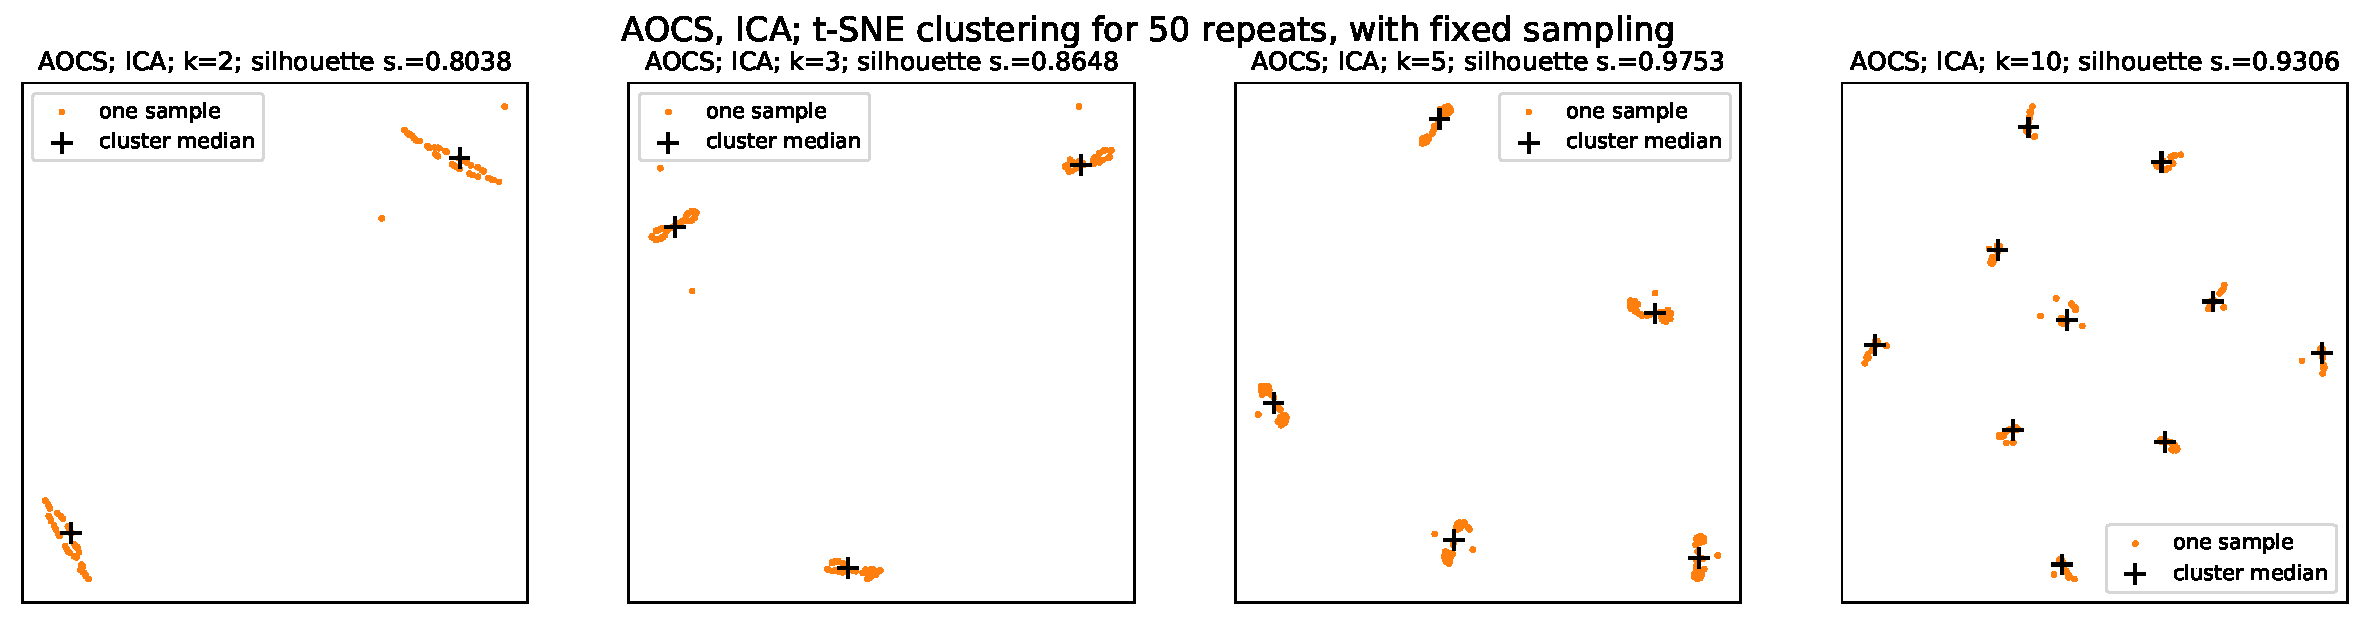
\includegraphics[scale=\S]{\plotspath{AOCS_Protein/FactorClustering/multiple_single_factors_scatter_AOCS_ICA_2_3_5_10_fixed.pdf}} \\
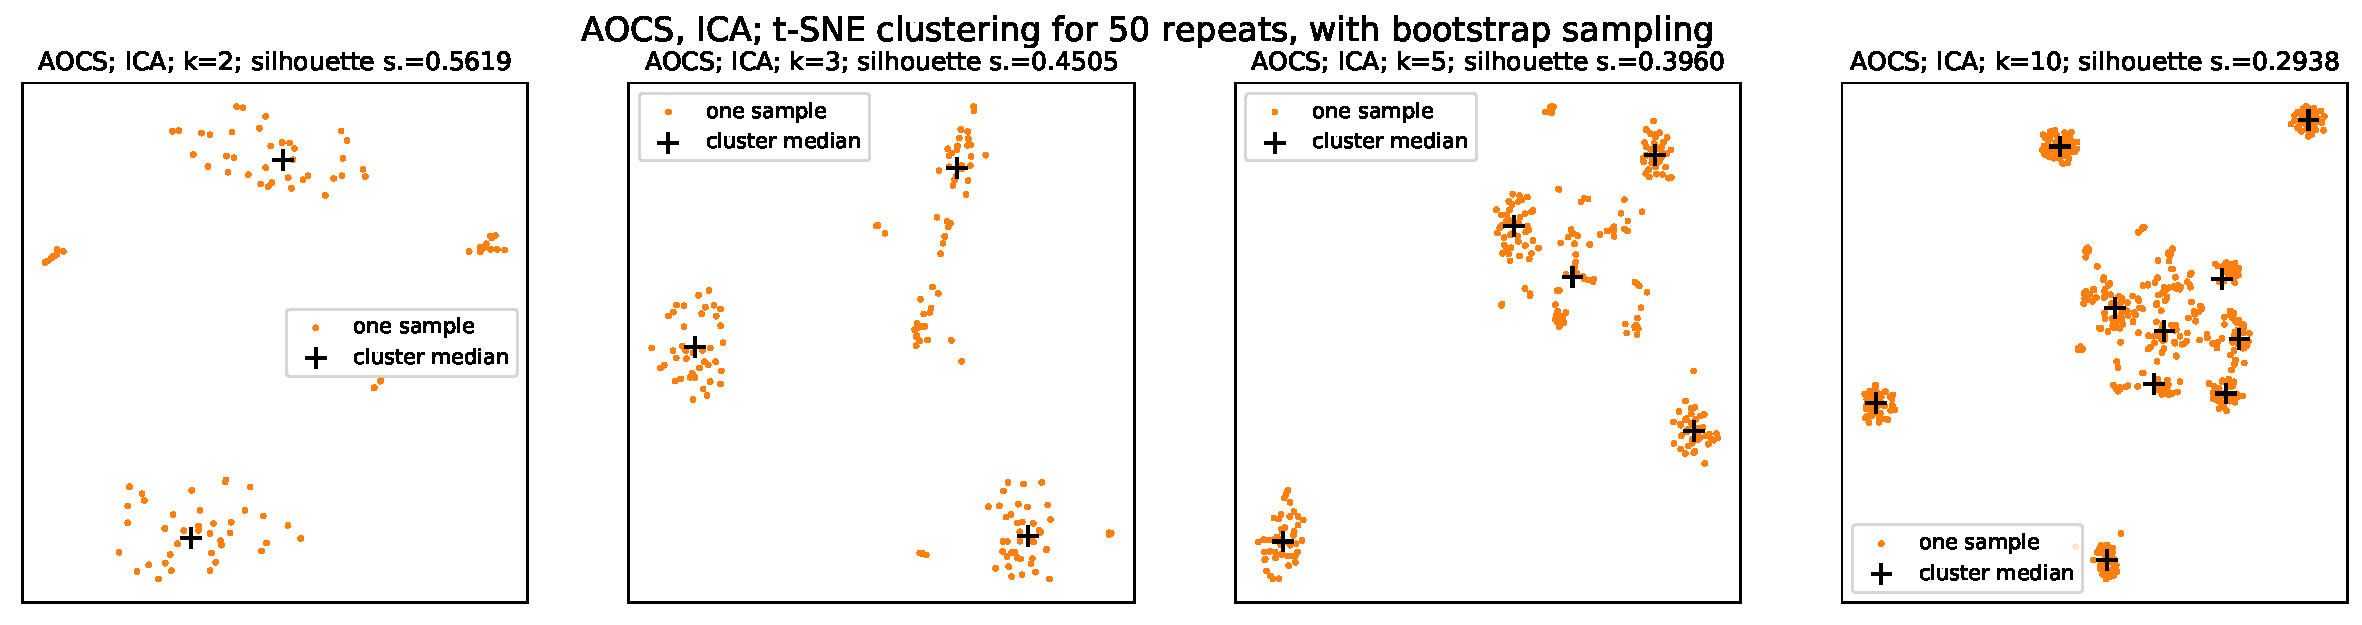
\includegraphics[scale=\S]{\plotspath{AOCS_Protein/FactorClustering/multiple_single_factors_scatter_AOCS_ICA_2_3_5_10_bootstrap.pdf}}\\
\caption{Clustering of metagenes from ICA facorizations on the N=80 AOCS dataset, comparing \emph{fixed} sampling (top row) with \emph{bootstrap} sampling (bottom row) for a selection of factorization ranks.  }
\label{fig-AOCS-ica-fixed-vs-bootstrap}
\label{fig-first-cluster-result}
\end{center}
\end{figure}

\begin{figure}[htb!]
\begin{center}
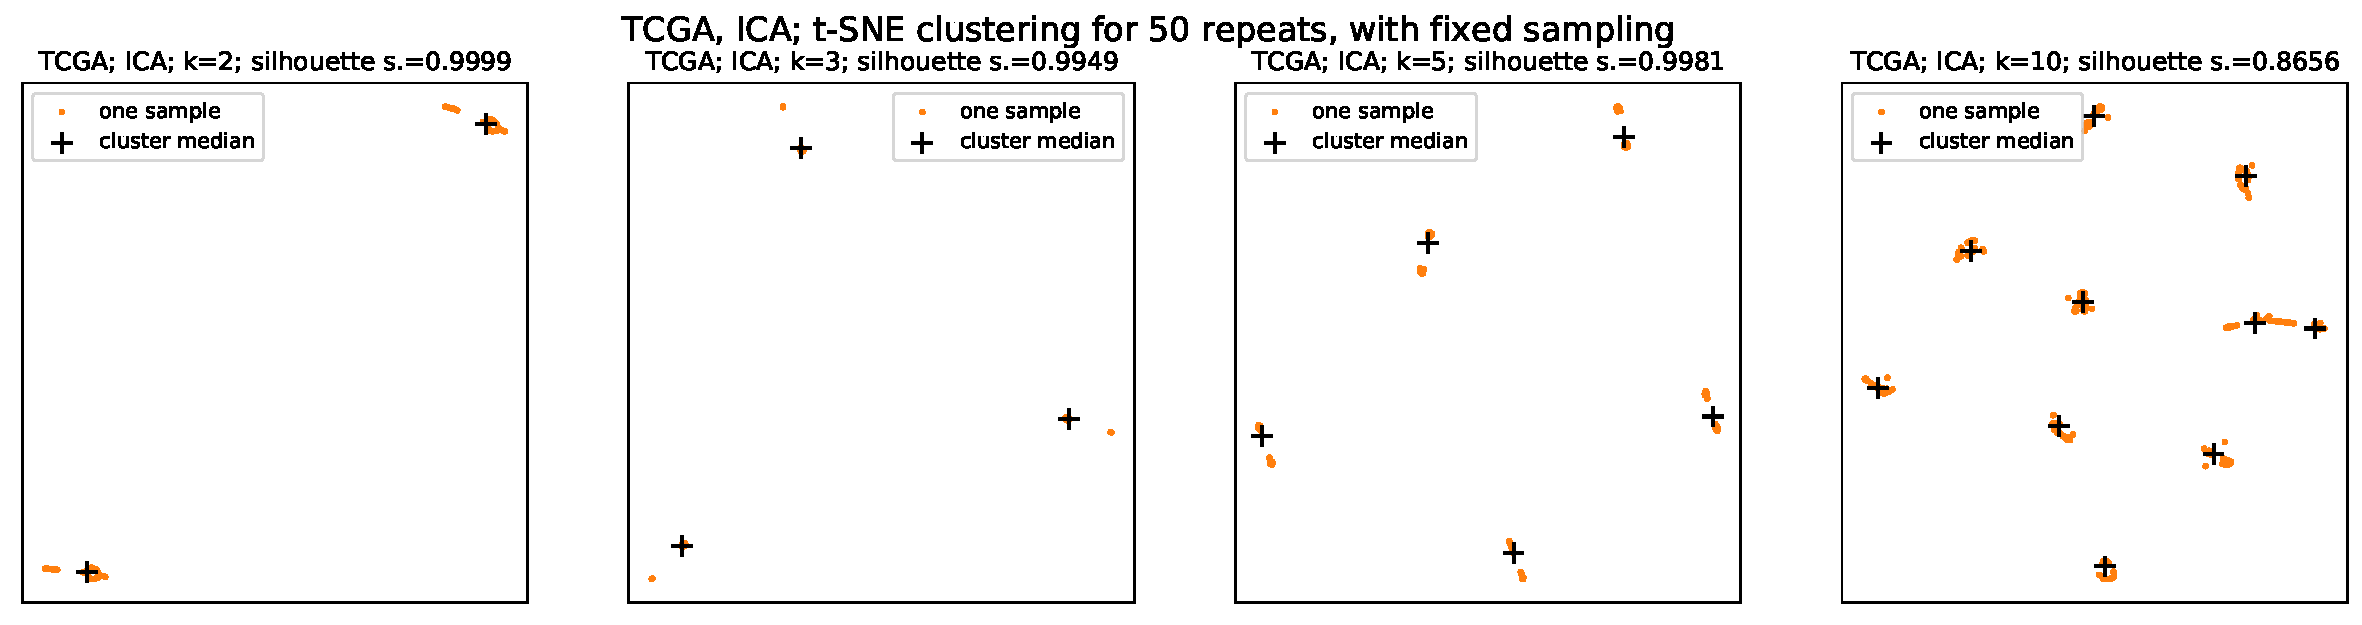
\includegraphics[scale=\S]{\plotspath{TCGA_OV_VST/FactorClustering/multiple_single_factors_scatter_TCGA_ICA_2_3_5_10_fixed.pdf}} 
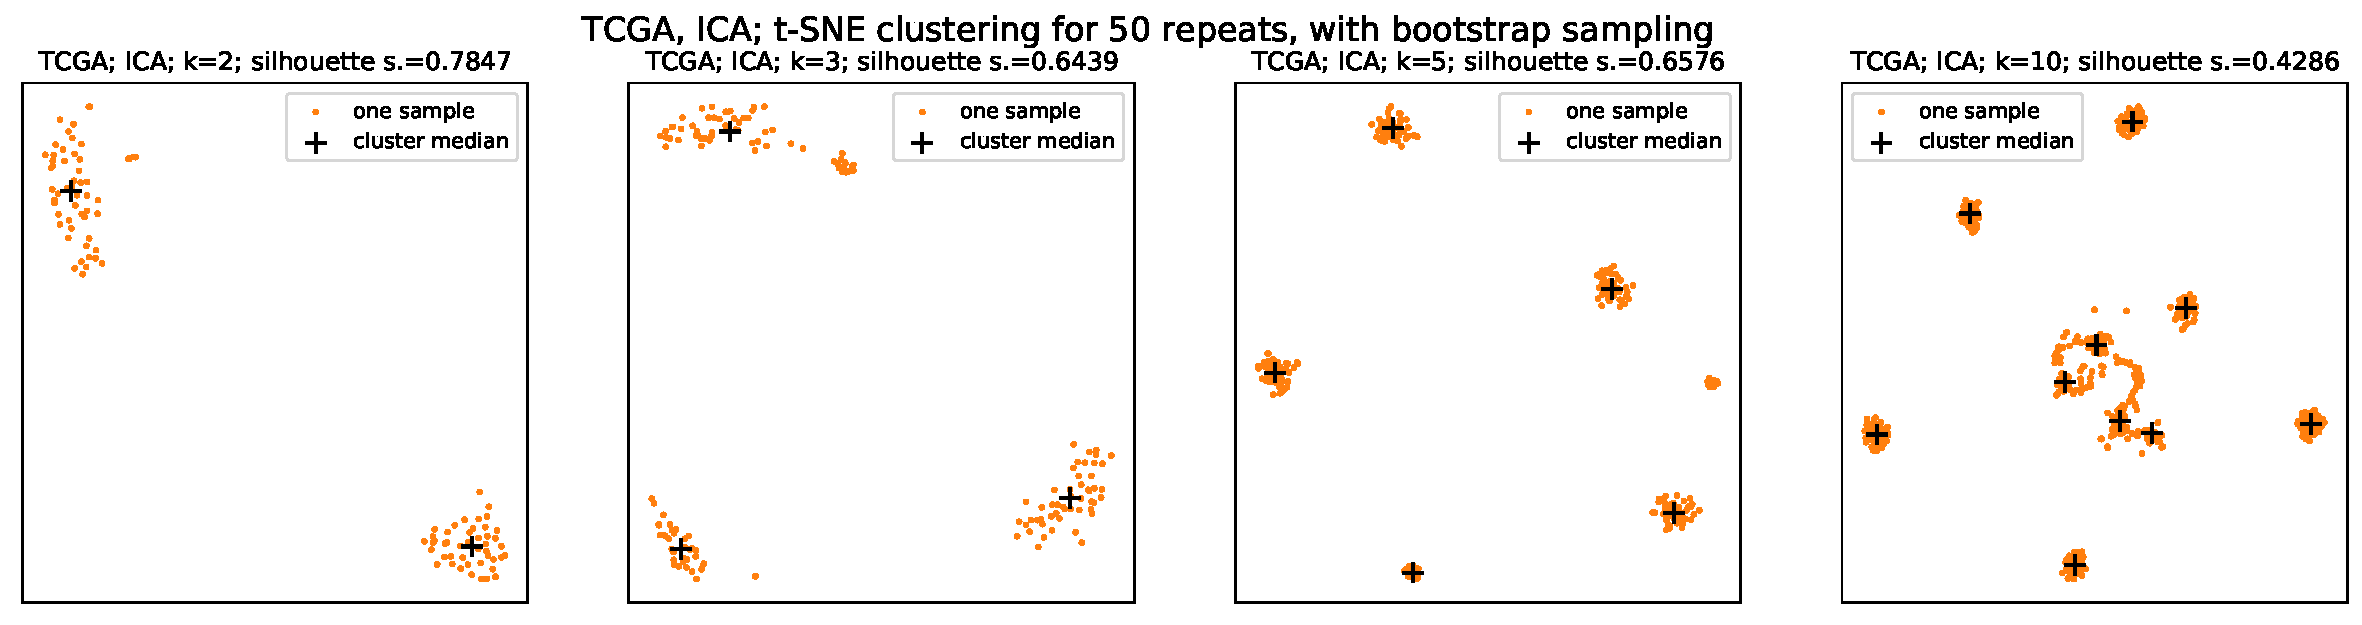
\includegraphics[scale=\S]{\plotspath{TCGA_OV_VST/FactorClustering/multiple_single_factors_scatter_TCGA_ICA_2_3_5_10_bootstrap.pdf}}
\caption{Clustering of metagenes from ICA facorizations on the N=374 TCGA dataset, again comparing fixed and bootstrap sampling.}
\label{fig-TCGA-ica-fixed-vs-bootstrap}
\end{center}
\end{figure}


In choosing the factorization rank for each method, both the t-SNE plots and silhouette scrore graphs in  figure \ref{fig-TCGA-all-bootstrap} were carefully considered.  
Firstly, $k>2$ is desirable to have sufficient information to work with.  NMF cluster coherence seems to deteriorate after $k=3$.   Looking at the graph of silhouette scores (figure \ref{fig-TCGA-all-bootstrap}, bottom), ICA appears to have a sweet spot at $k=5$.  For PCA, $k = 3$ or $4$ both seem reasonable.
As already noted earlier, the following choices were made:
$K_{\mbox{\tiny NMF}}  =  3,
K_{\mbox{\tiny ICA}}  =  5,
K_{\mbox{\tiny PCA}}  =  3$.

There is a curious artefact visible in the NMF factorization clusterings of figure \ref{fig-TCGA-all-bootstrap}, top row.  For $k=2, 3$ and $5$ several of the clusters show a bi-modal character.  This is not observed in the fixed sampling case (not shown).  The artefact is difficult to explain.  It cannot be the $180^\circ$ rotation issue discussed earlier, since this does not apply to the all +ve components; I have no explanation.

\begin{figure}[htb!]
\begin{center}
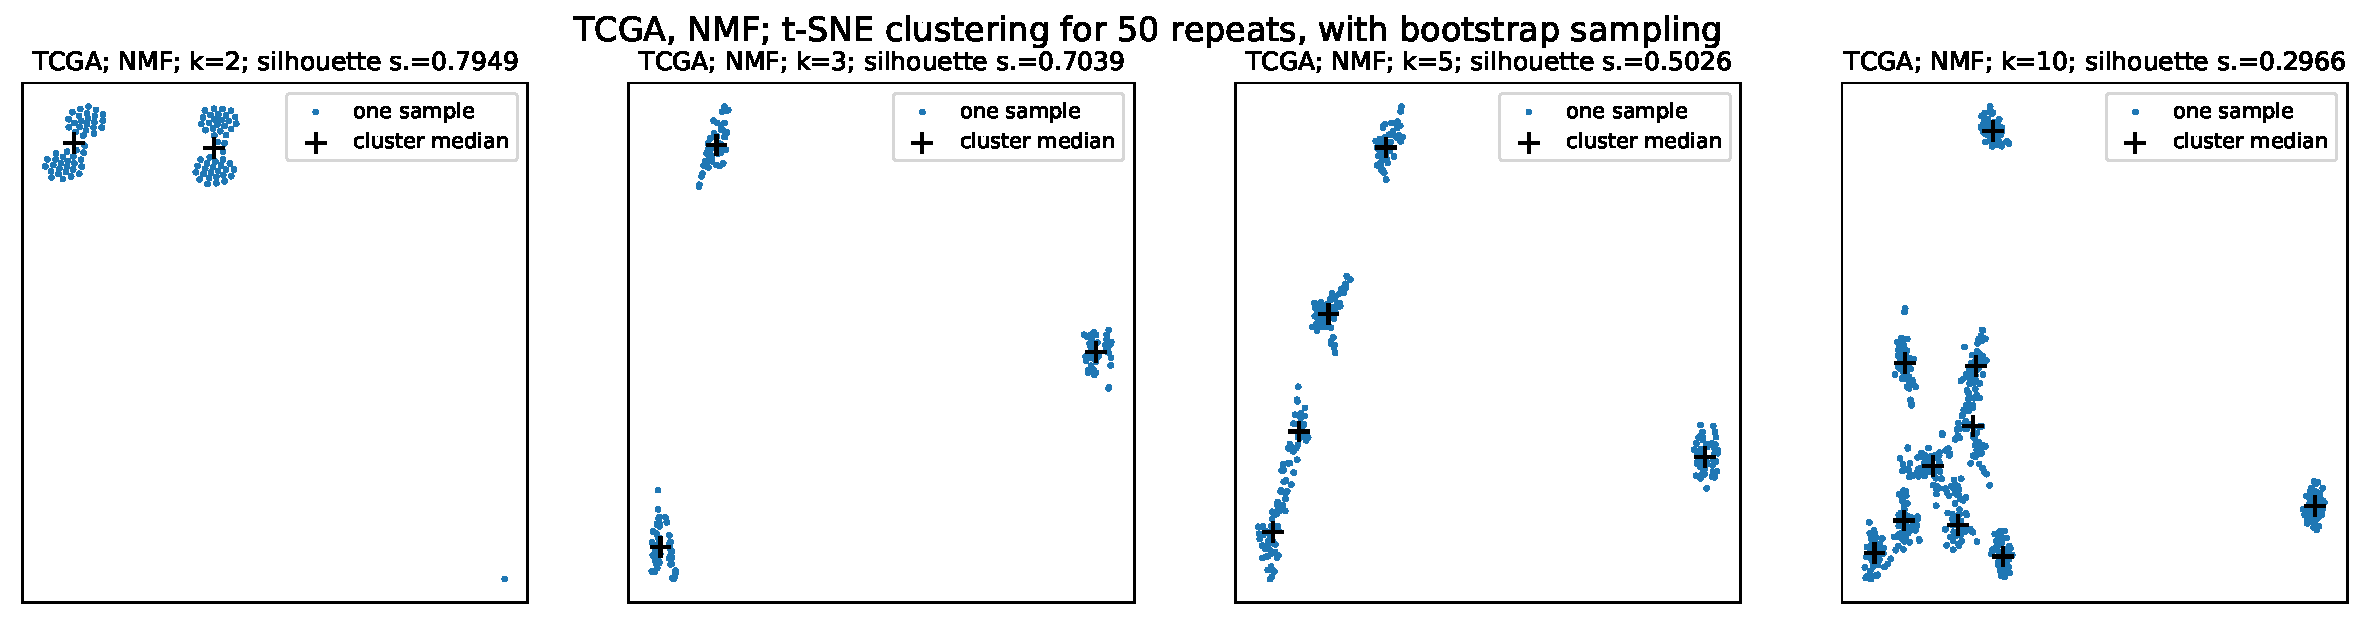
\includegraphics[scale=\S]{\plotspath{TCGA_OV_VST/FactorClustering/multiple_single_factors_scatter_TCGA_NMF_2_3_5_10_bootstrap.pdf}} \\
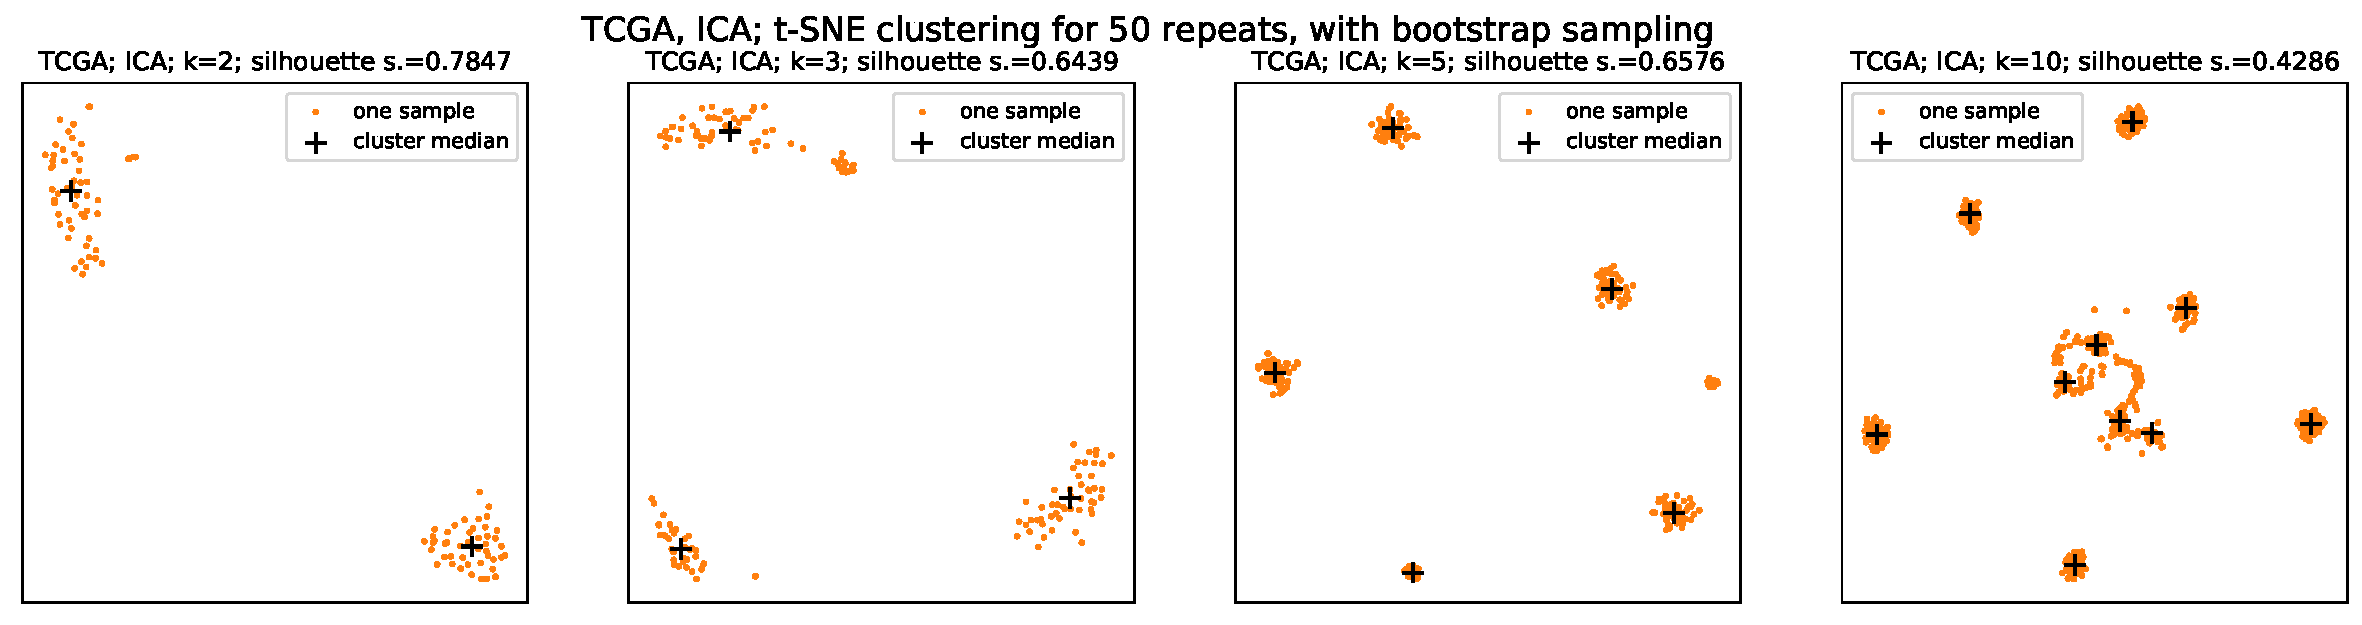
\includegraphics[scale=\S]{\plotspath{TCGA_OV_VST/FactorClustering/multiple_single_factors_scatter_TCGA_ICA_2_3_5_10_bootstrap.pdf}} \\
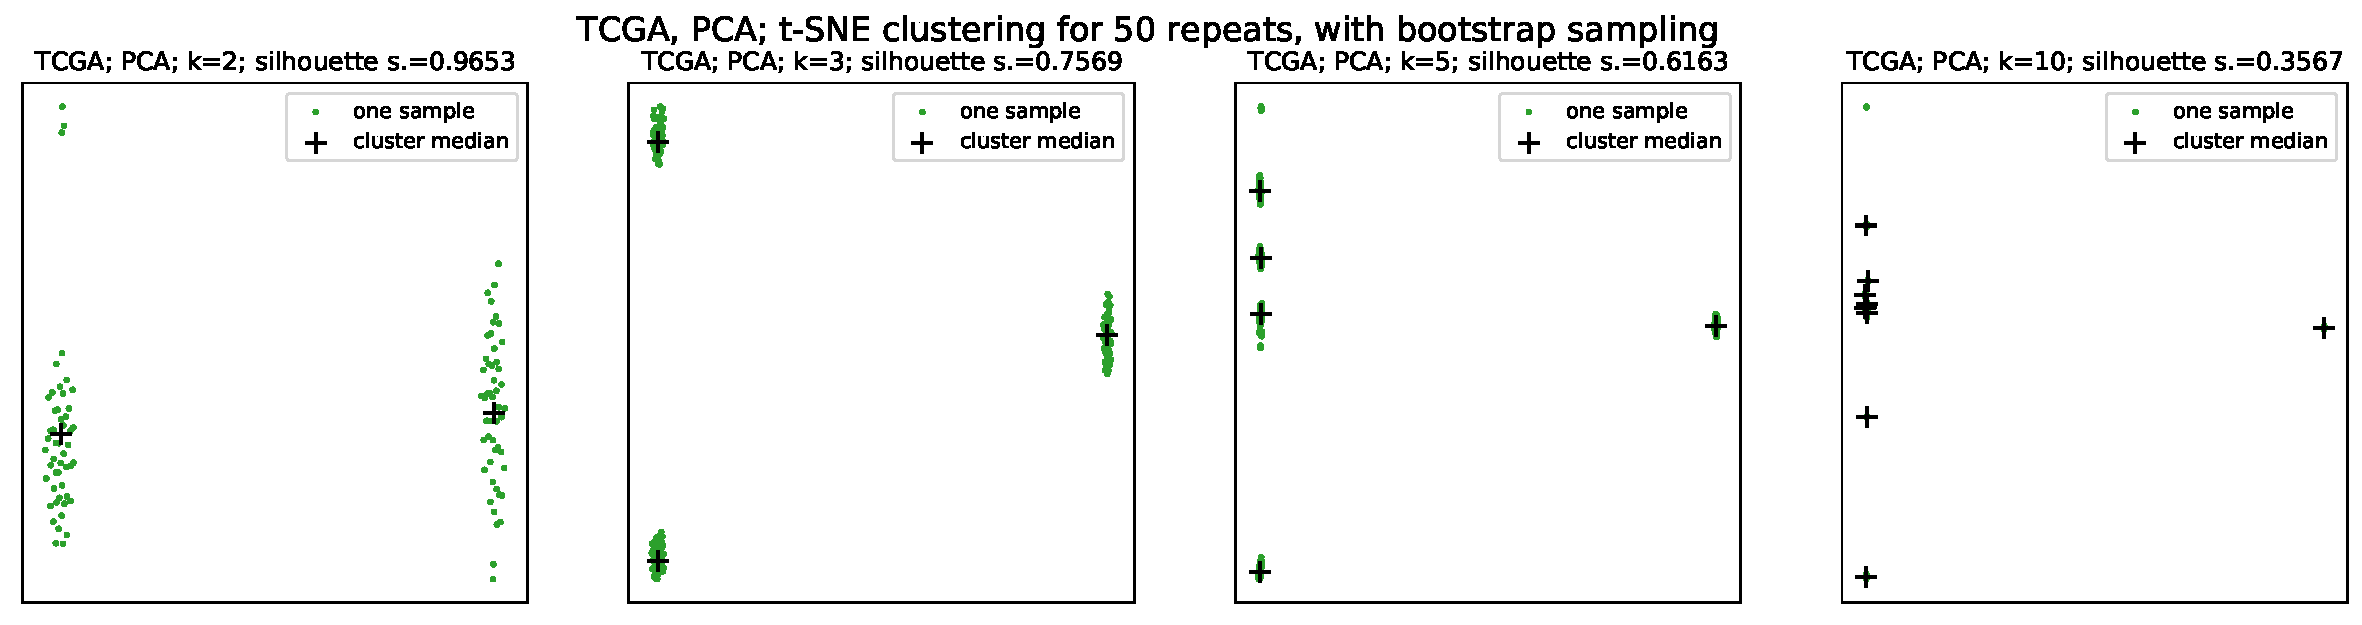
\includegraphics[scale=\S]{\plotspath{TCGA_OV_VST/FactorClustering/multiple_single_factors_scatter_TCGA_PCA_2_3_5_10_bootstrap.pdf}} \\
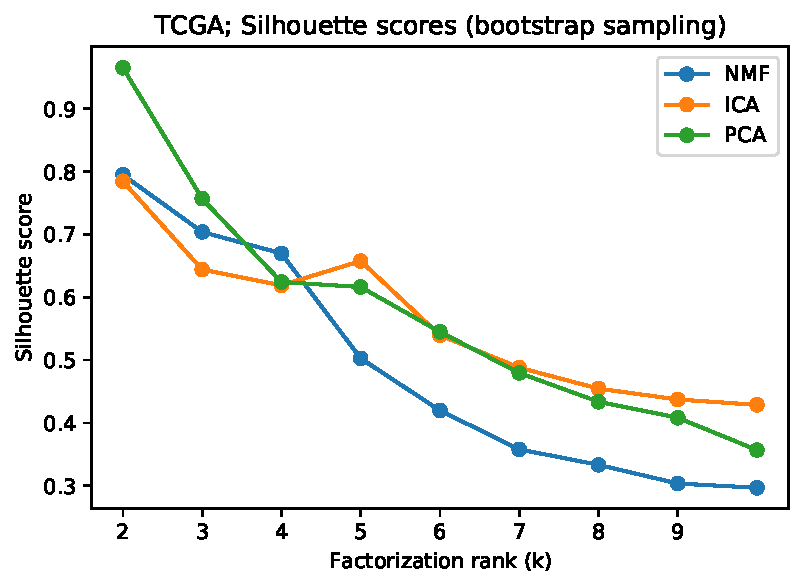
\includegraphics[scale=0.55]{\plotspath{/TCGA_OV_VST/FactorClustering/silhouette_plots_TCGA_2_3_4_5_6_7_8_9_10_bootstrap.pdf}} 
\caption{Metagene clustering for all three methods applied to the N=374 TCGA dataset with bootstrap sampling, over a range of factorization ranks.  The silhouette scores are also plotted (bottom).  It is on the basis of this figure that the factorization ranks for each method were selected.}
\label{fig-TCGA-all-bootstrap}
\label{fig-last-cluster-result}
\end{center}
\end{figure}

\FloatBarrier

\subsection{Jaccard similarity shows metagenes identify intersecting gene sets in some cases}

The Jaccard heatmap of figure \ref{fig-component-jaccard-similarities} shows that some pairs of metagenes identify overlapping sets of genes, in particular the pairs (ICA-1, PCA-2: J=0.61) and (ICA-5, PCA-3: J=0.49).  As expected however, there is very little similarity between components \emph{within} a factorization method.

\begin{figure}[htb!]
\begin{center}
\includegraphics[scale=0.4]{\plotspath{TCGA_OV_VST/GeneEnrichment/component_jaccard_heatmap.pdf}}
\end{center}
\caption{Heatmap of Jaccard similarities between the candidate genes identified by the 11 components.}
\label{fig-component-jaccard-similarities}
\end{figure}

\FloatBarrier

\subsection{Metagenes highlight genes which are enriched for biological processes}

GEA against the GO results in, for each of the 11 metagenes, a table of GO terms with a list of the candidate genes which have an annotated association to that term. See appendix \ref{tab-go-enrichment-results} to access the full table.
To take full advantage of the hierarchical nature of the GO, results are presented as lineage maps in figures \ref{fig-NMF_1-go-lineage} to \ref{fig-PCA-3-3-go-lineage}.   (The large graphic for ICA-4 is in the appendix, figure \ref{fig-ICA-4-go-lineage}).
The contributing candidate genes for all significantly enriched terms are shown beneath each figure.  
High-level terms at depth less than 3 were removed, since these are generic (e.g. ``regulation of biological process") and so uninteresting.   
One component -- ICA-4 -- was problematic in that 49 GO terms (with depth $\geq 3$) were identified as significant.  
For this component it was necessary to limit the graphic to the 12 terms having the largest number of associated candidate genes.   

The four components NMF-3, ICA-1, ICA-2 and PCA-2 yielded no significant enriched terms (for FDR $\leq$ 0.01).

\begin{figure}[htb!]
\begin{center}
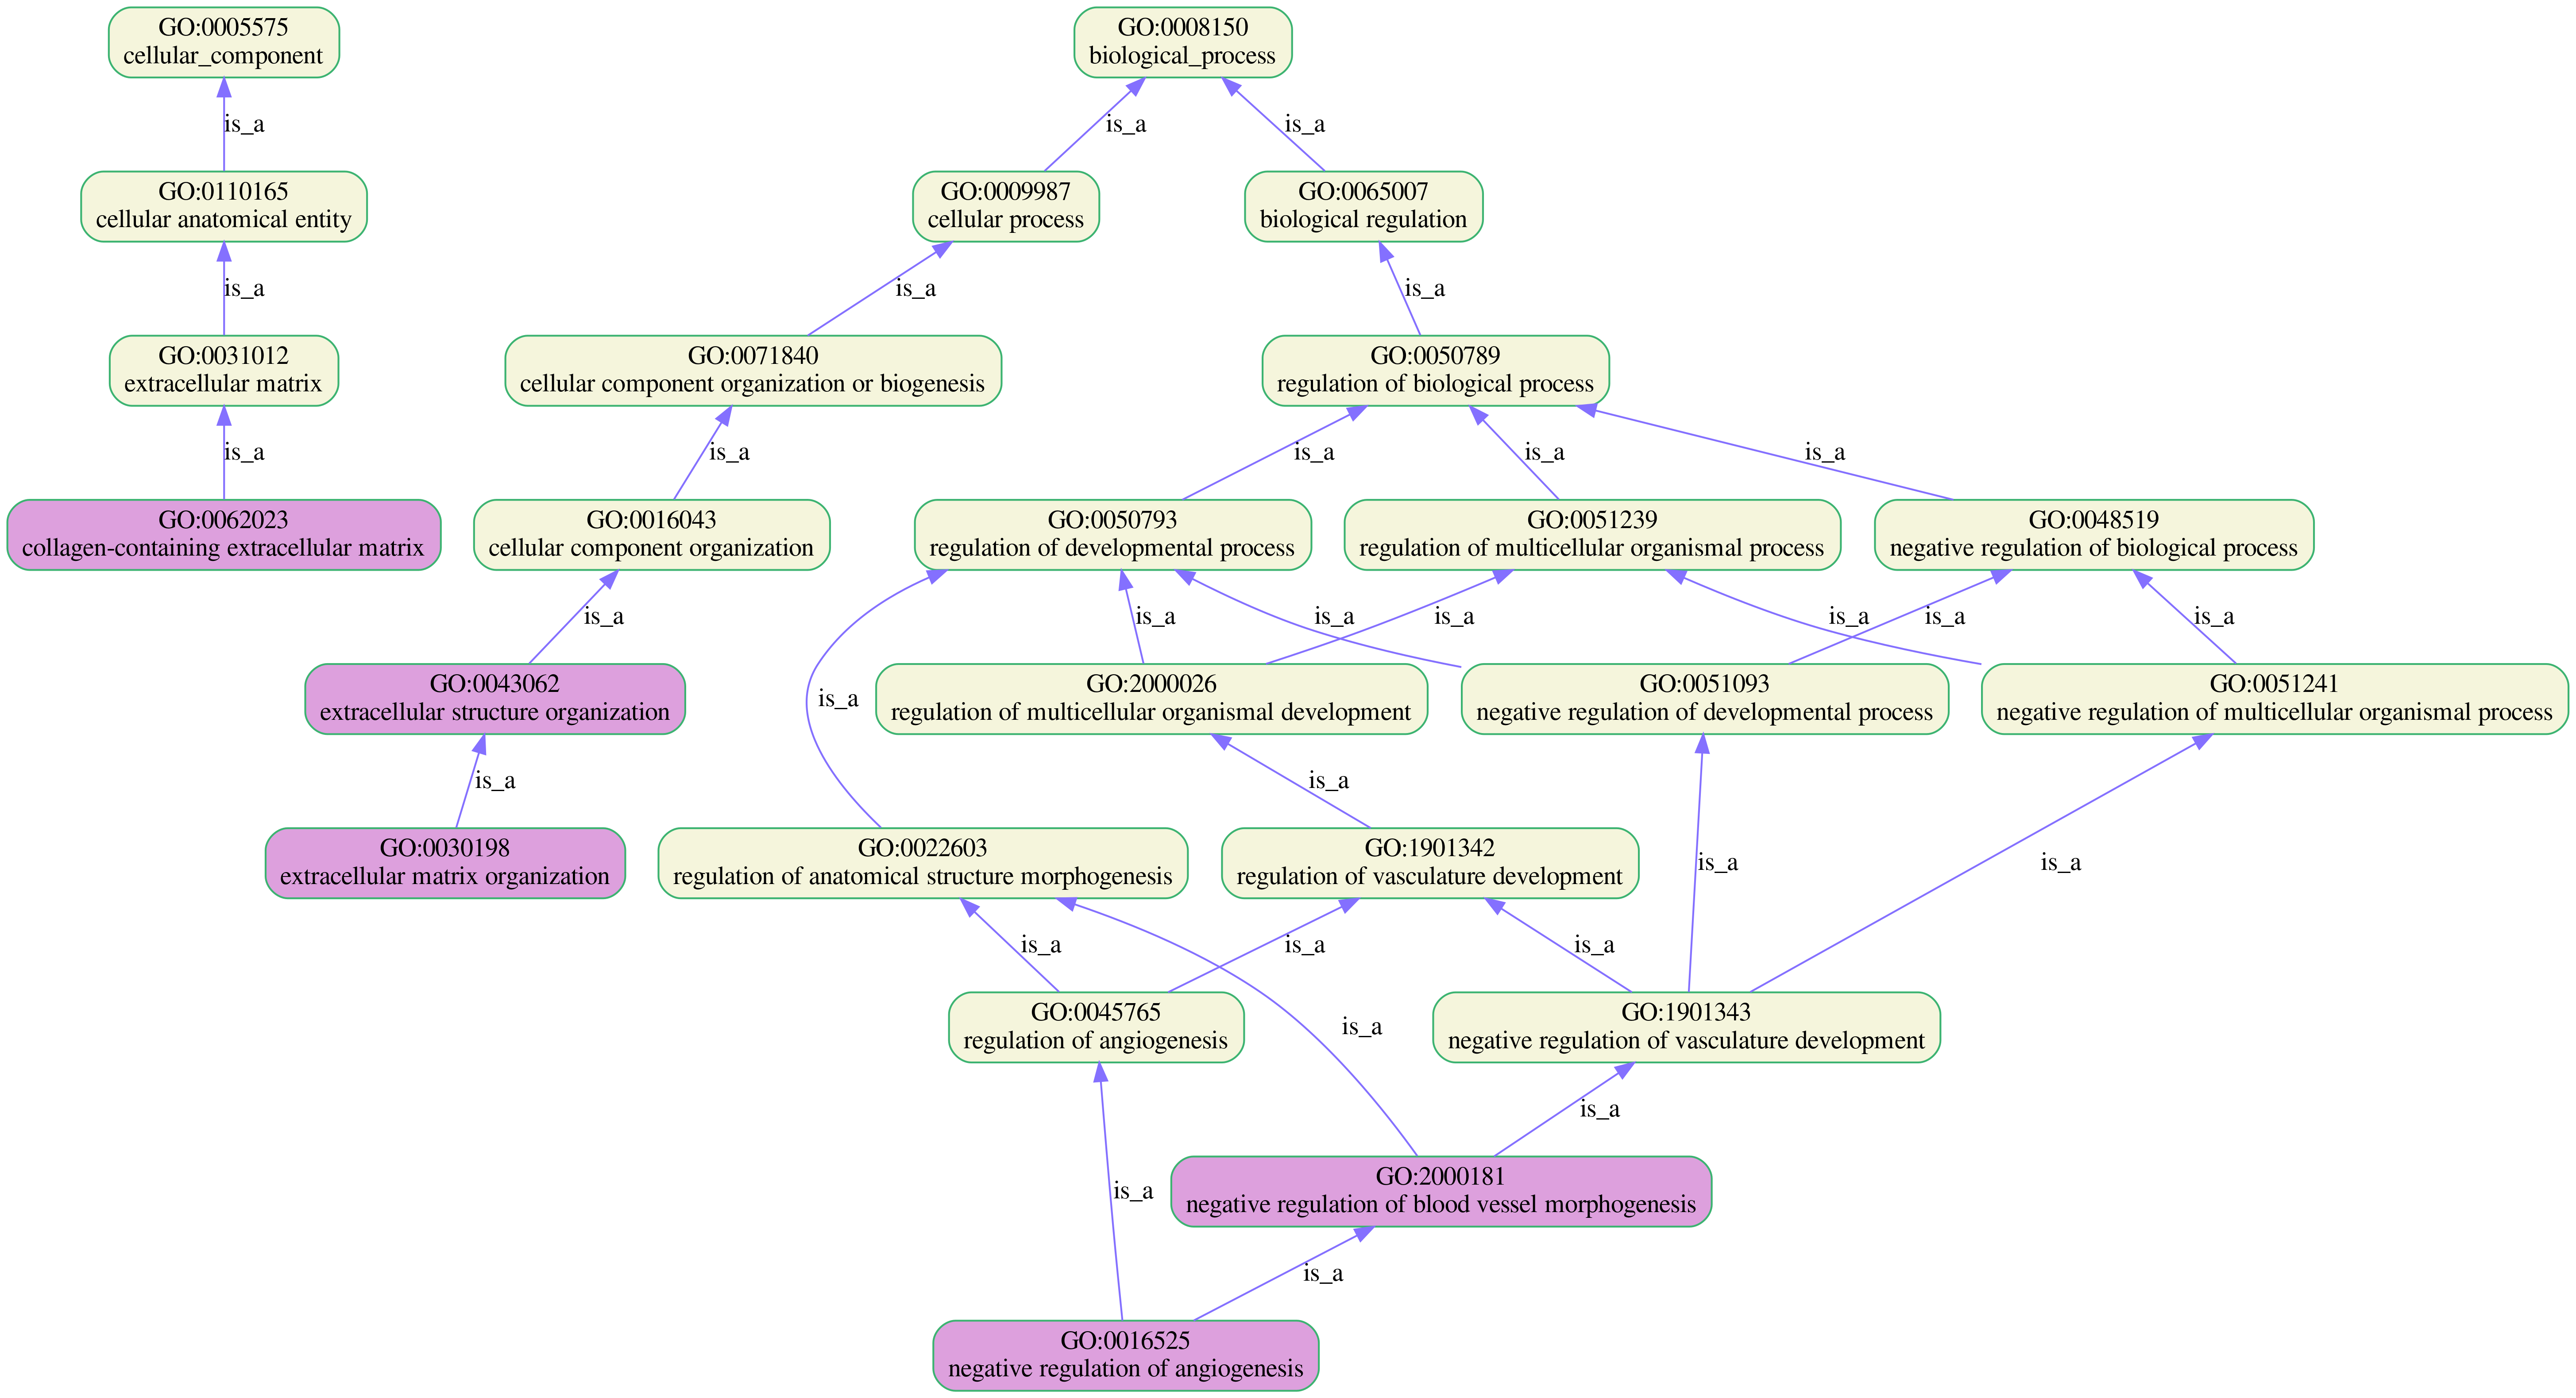
\includegraphics[scale=0.08]{\plotspath{TCGA_OV_VST/GeneEnrichment/go_lineage_1_of_NMF_3.png}} \\
\begin{spacing}{0.6}
{\small Genes: \tiny \input{/home/ipoole/Documents/gitrepos/HgsocTromics/Plots/TCGA_OV_VST/GeneEnrichment/go_gene_set_1_of_NMF_3.txt}}
\end{spacing}
\vspace{0.5cm}
{\small Component NMF-1} \\
\end{center}
\caption{Lineage maps of enriched Gene Ongology (GO) terms for components NMF-1  In these diagrams, enriched terms are coloured purple, while there ancestors in the ontology are yellow.  }
\label{fig-NMF_1-go-lineage}
\end{figure}

\begin{figure}[htb!]
\begin{center}
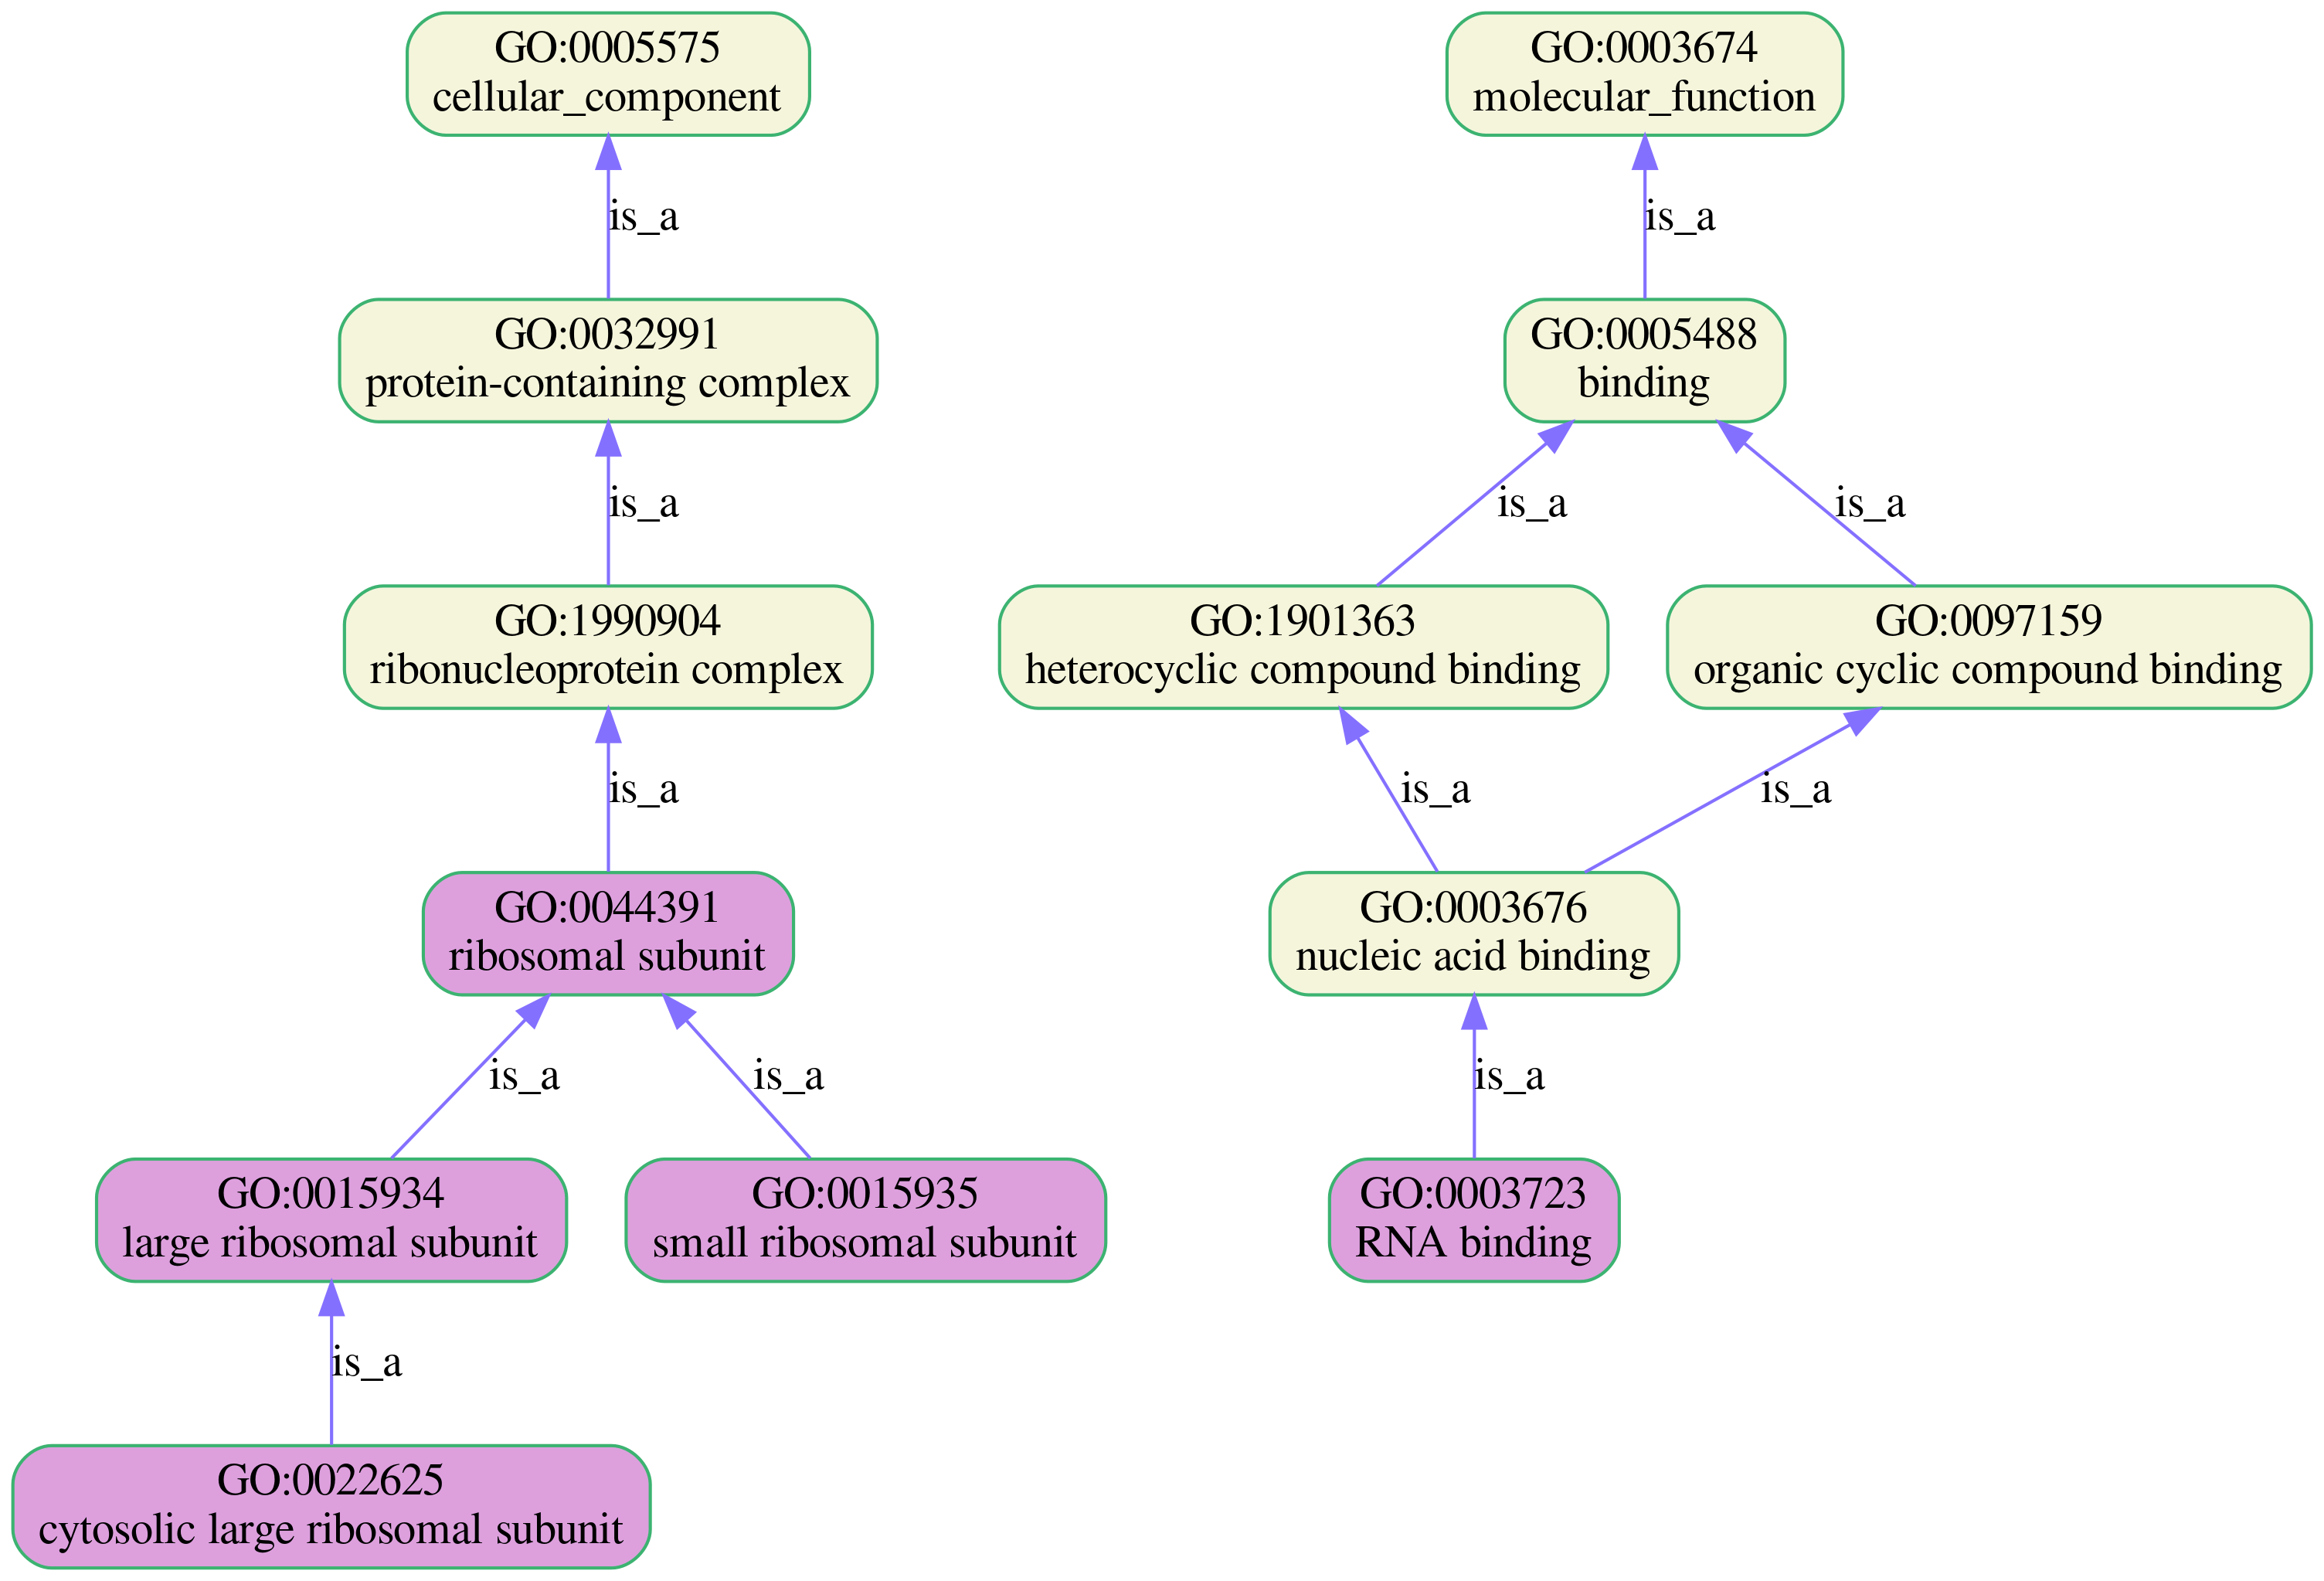
\includegraphics[scale=0.1]{\plotspath{TCGA_OV_VST/GeneEnrichment/go_lineage_2_of_NMF_3.png}} \\
\begin{spacing}{0.6}
{\small Genes: \tiny \input{/home/ipoole/Documents/gitrepos/HgsocTromics/Plots/TCGA_OV_VST/GeneEnrichment/go_gene_set_2_of_NMF_3.txt}}
\end{spacing}
\vspace{0.5cm}
{\small Component NMF 2} \\
\caption{Lineage maps of enriched GO terms for components NMF-2.   (NMF-3 produced no significant enrichment results)}
\label{fig-NMF_2-go-lineage}
\end{center}
\end{figure}


\begin{figure}[htb!]
\begin{center}
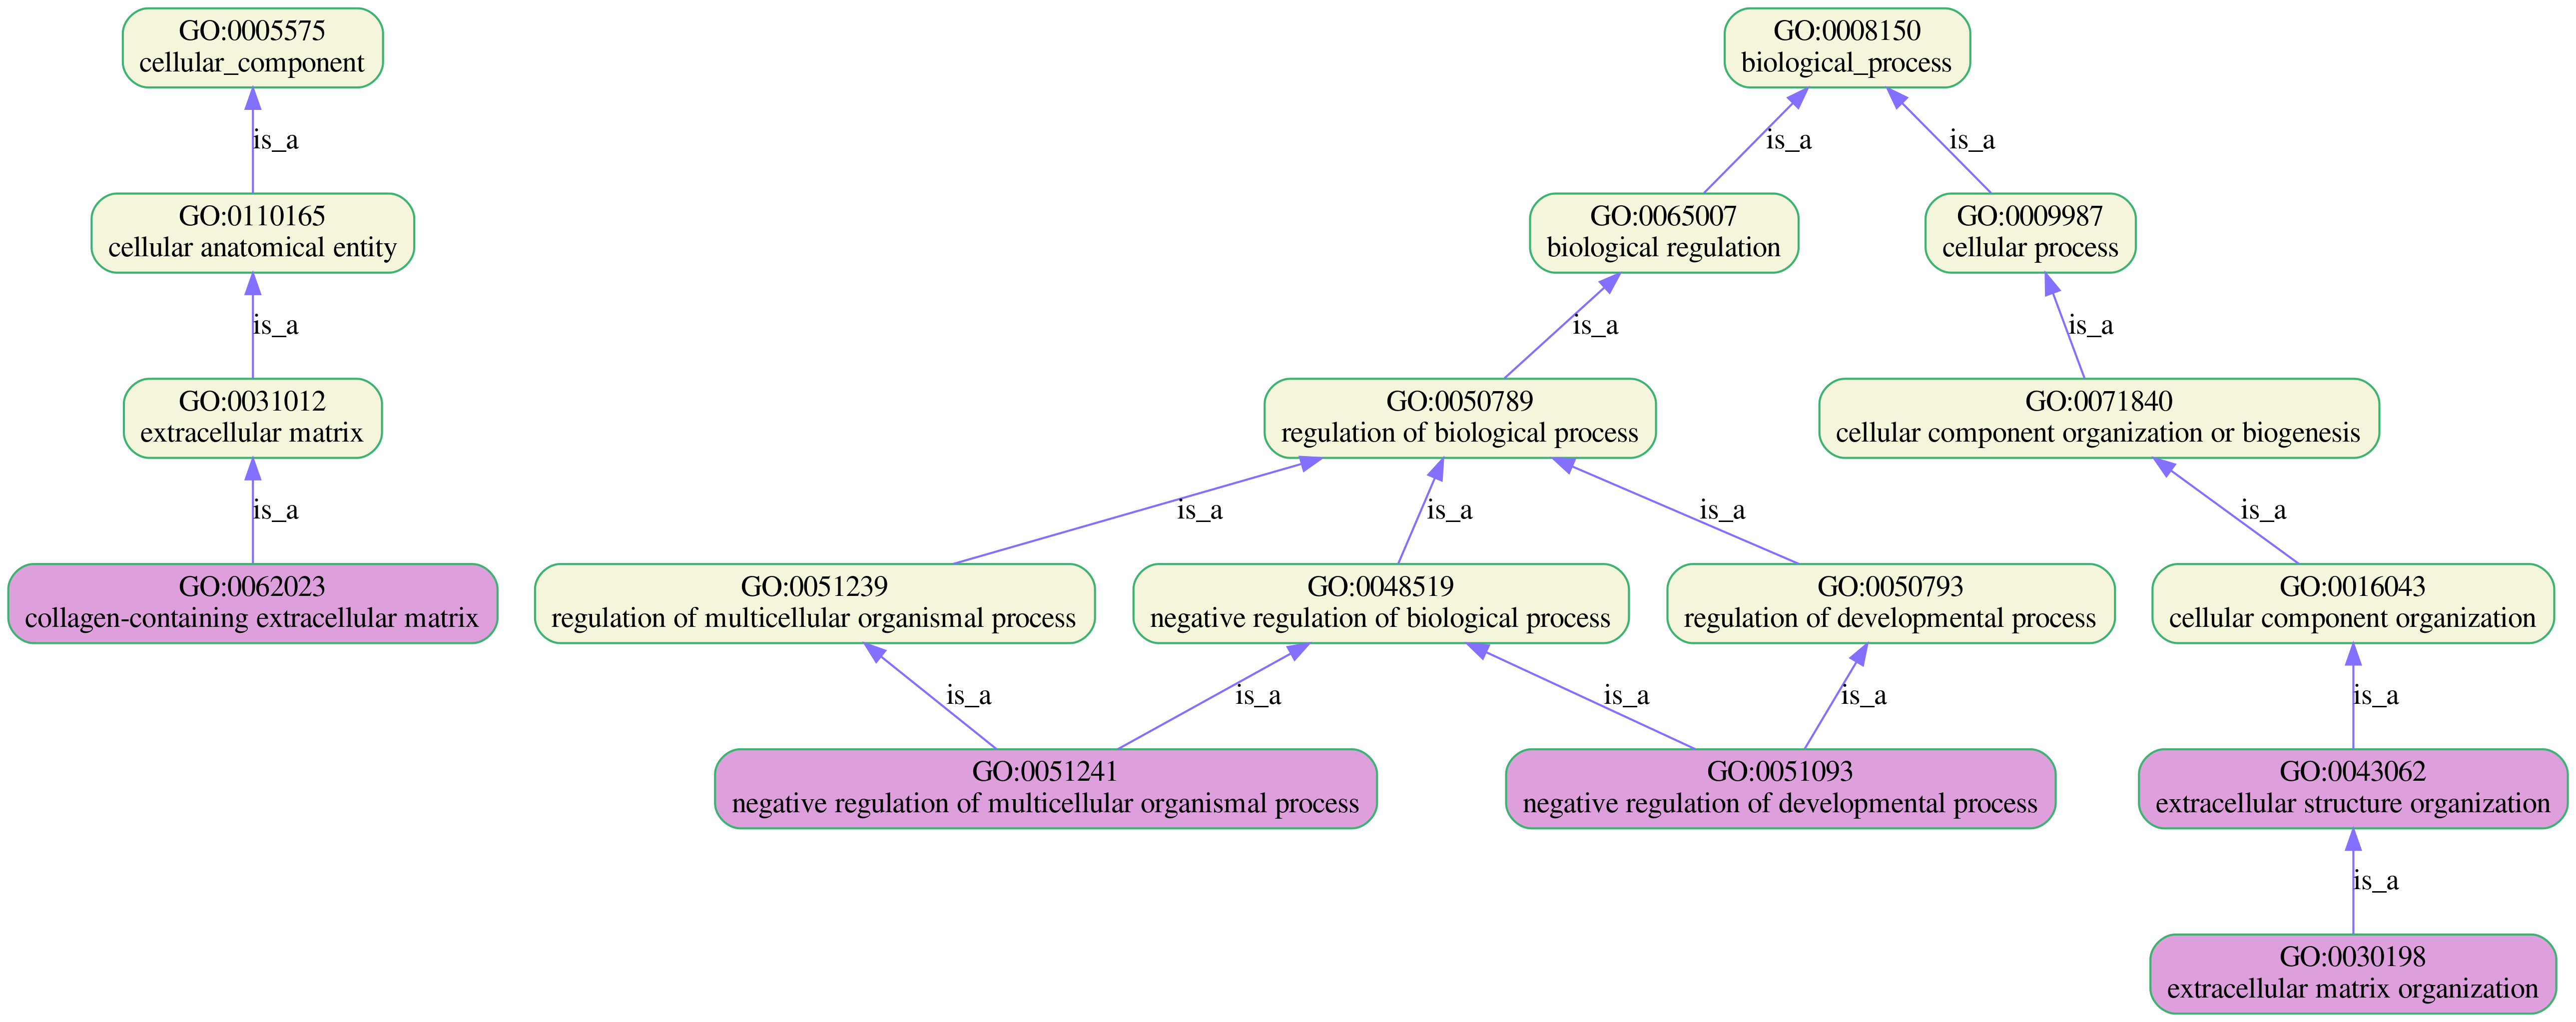
\includegraphics[scale=0.09]{\plotspath{TCGA_OV_VST/GeneEnrichment/go_lineage_3_of_ICA_5.png}} \\
\begin{spacing}{0.6}
{\small Genes: \tiny \input{/home/ipoole/Documents/gitrepos/HgsocTromics/Plots/TCGA_OV_VST/GeneEnrichment/go_gene_set_3_of_ICA_5.txt}}
\end{spacing}
\vspace{0.5cm}
{\small Component ICA-3} \\
\end{center}
\caption{Lineage maps of enriched GO terms for components ICA-3}
\label{fig-ICA-3-5-go-lineage}
\end{figure}

\begin{figure}[htb!]
\begin{center}
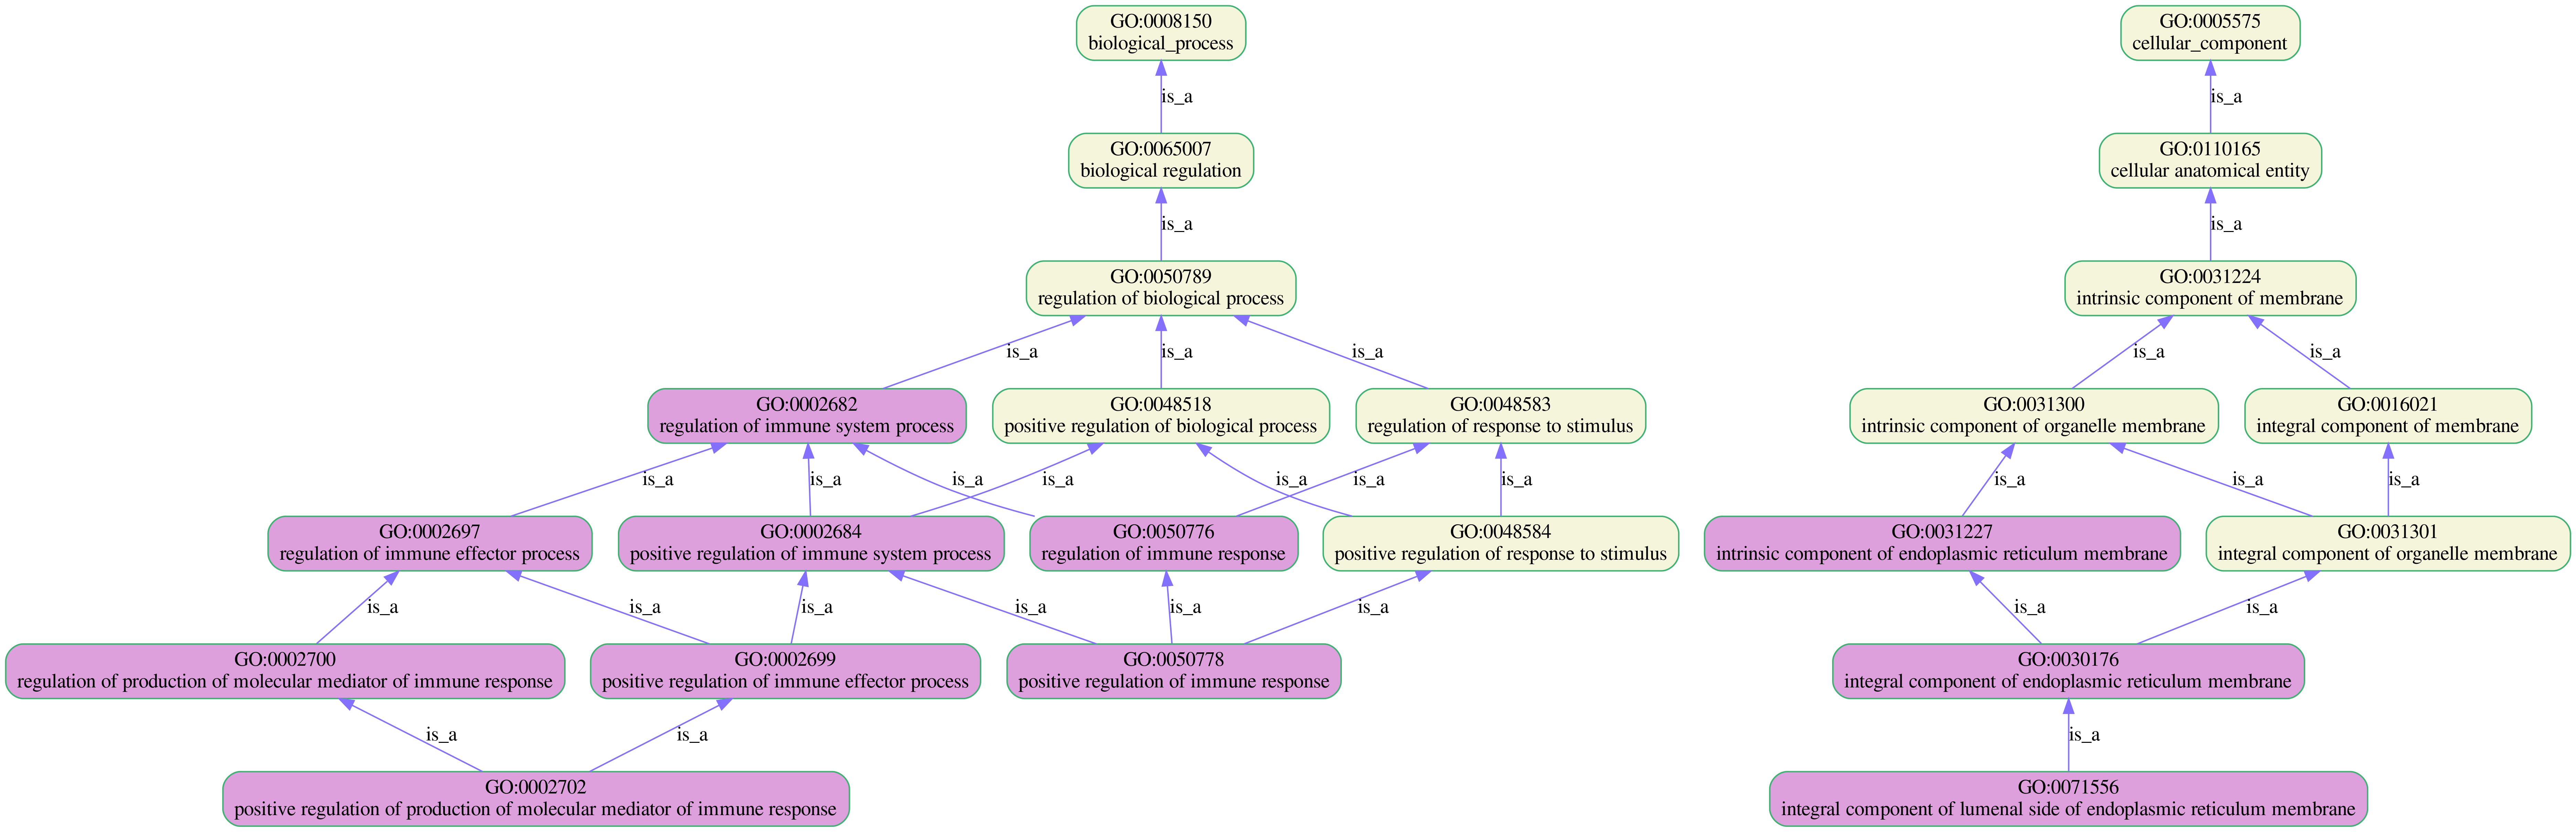
\includegraphics[scale=0.06]{\plotspath{TCGA_OV_VST/GeneEnrichment/go_lineage_5_of_ICA_5.png}} \\
\begin{spacing}{0.6}
{\small Genes: \tiny \input{/home/ipoole/Documents/gitrepos/HgsocTromics/Plots/TCGA_OV_VST/GeneEnrichment/go_gene_set_5_of_ICA_5.txt}}
\end{spacing}
\vspace{0.5cm}
{\small Component ICA-5} \\
\caption{Lineage maps of enriched GO terms for components ICA-5}
\label{fig-ICA-5-5-go-lineage}
\end{center}
\end{figure}


\begin{figure}[htb!]
\begin{center}
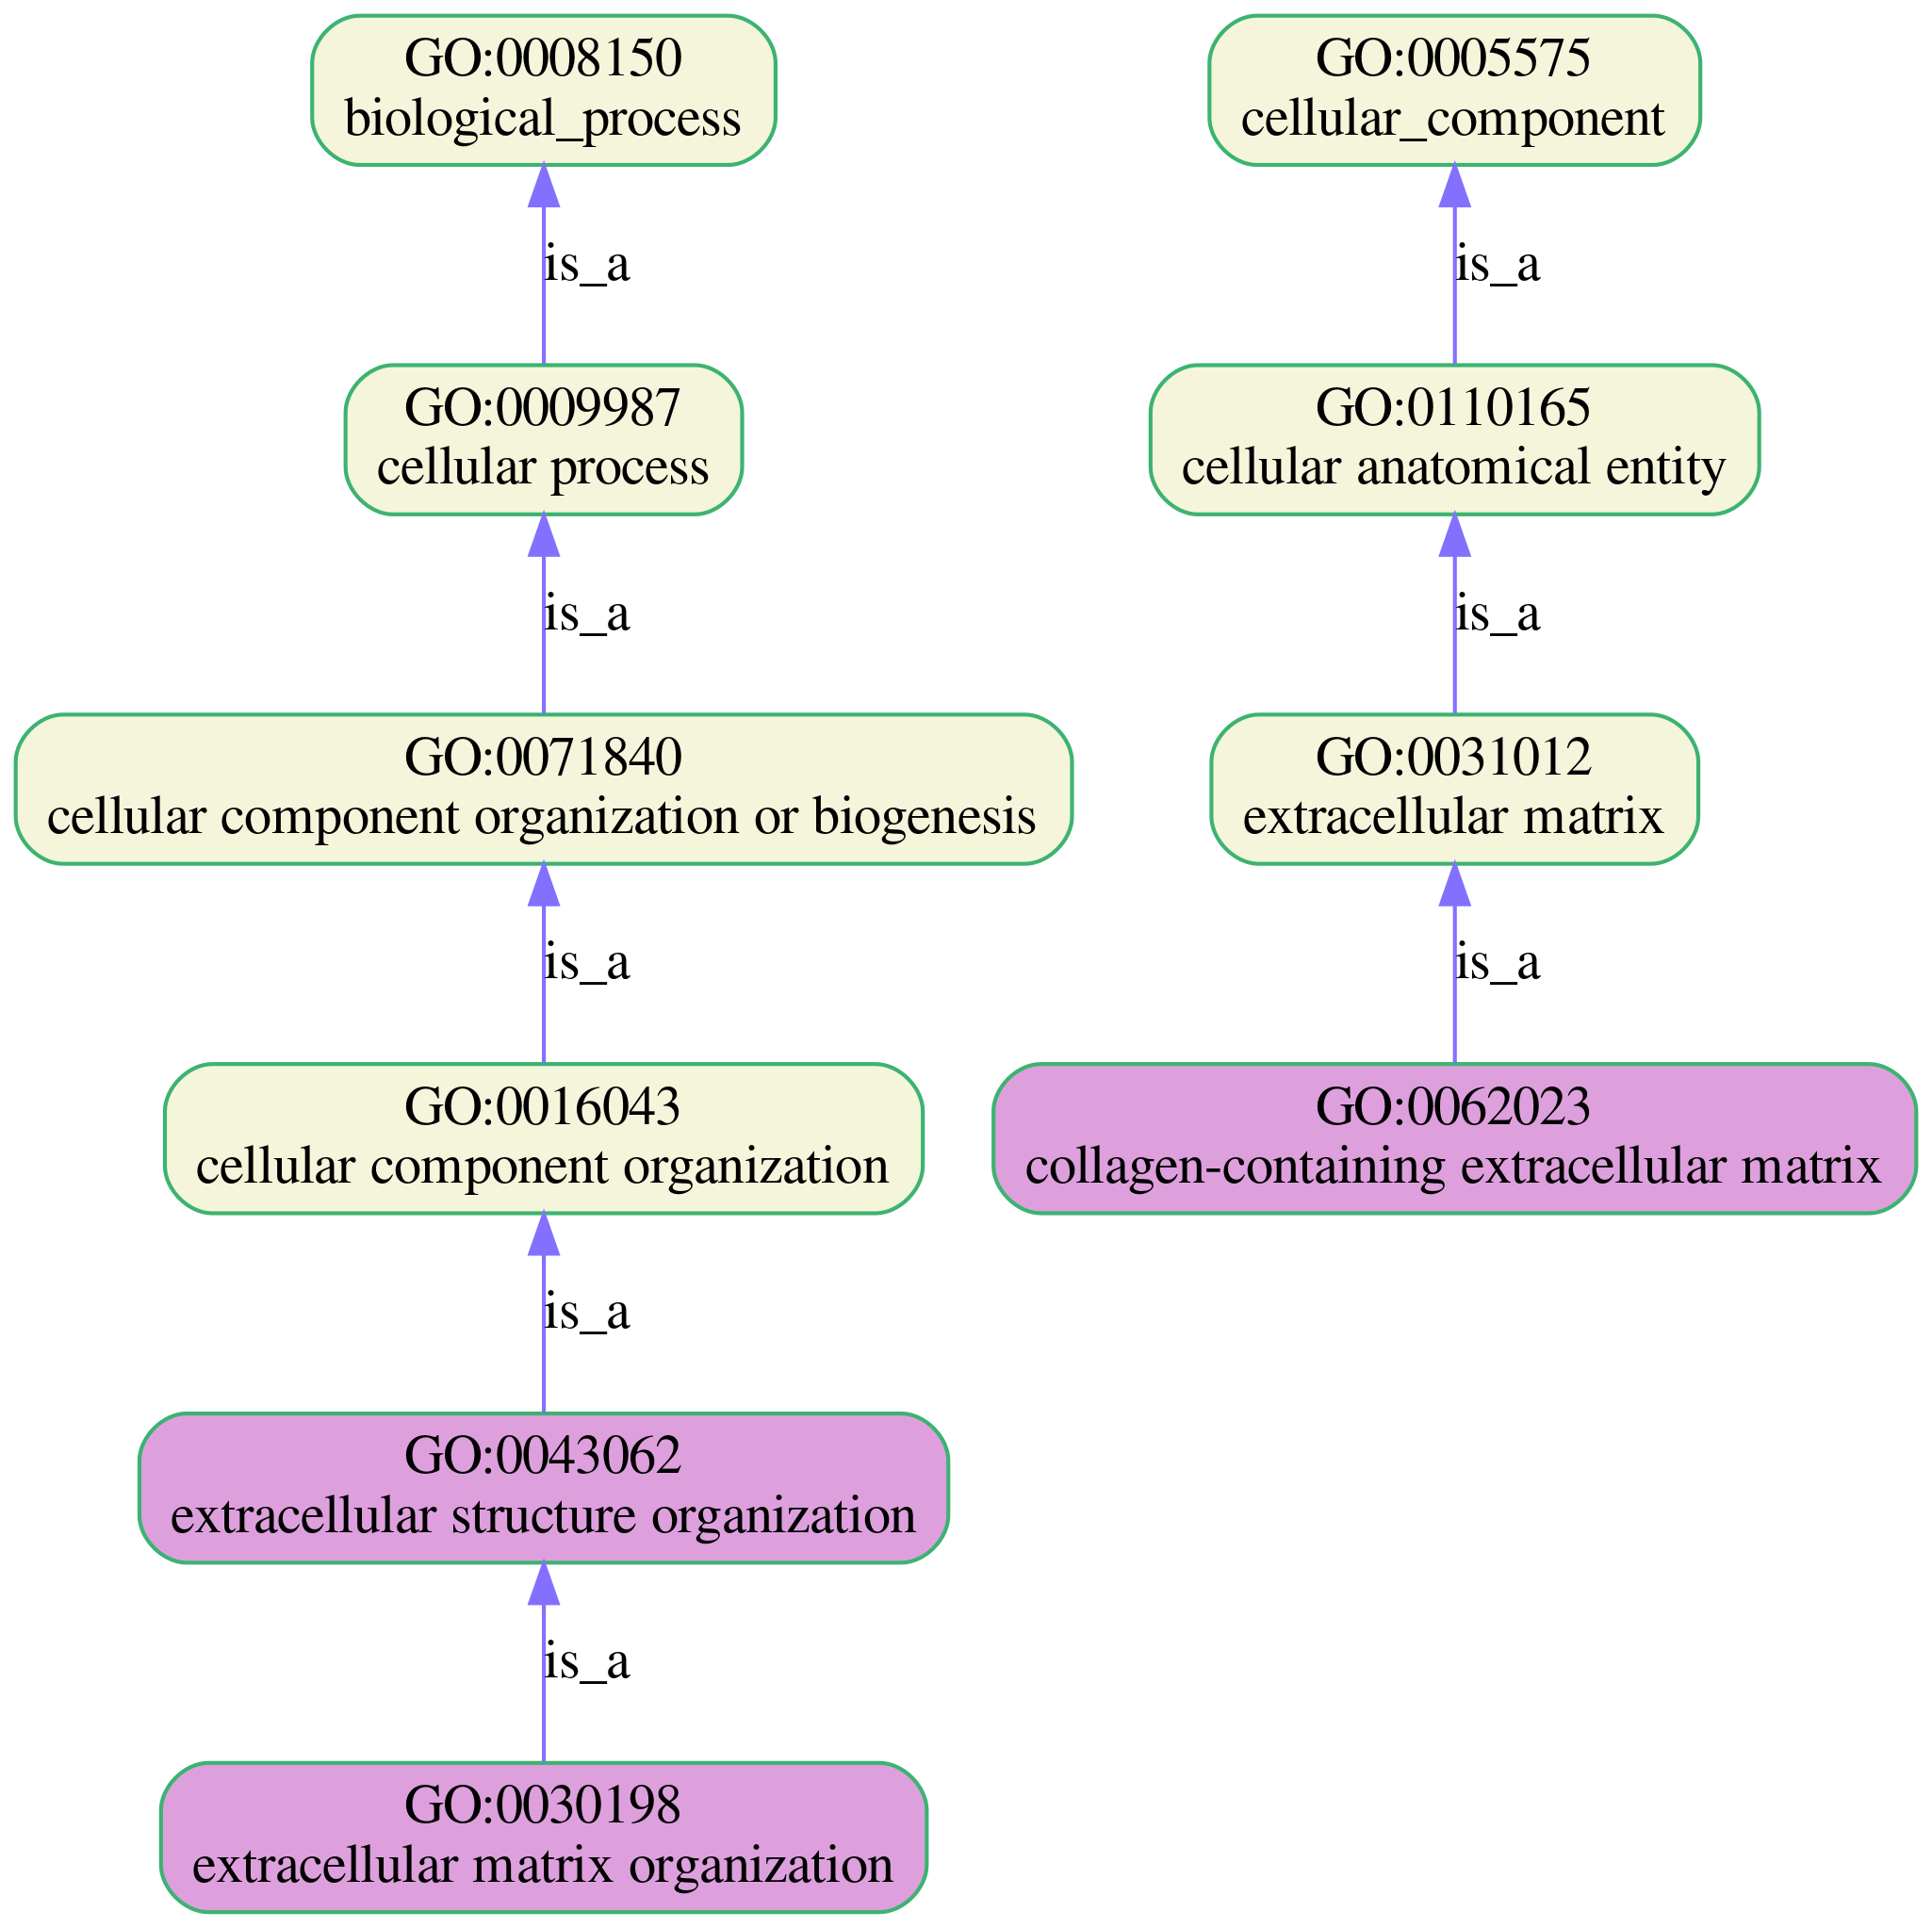
\includegraphics[width=0.4 \textwidth]{\plotspath{TCGA_OV_VST/GeneEnrichment/go_lineage_1_of_PCA_3.png}} \\
\begin{spacing}{0.6}
{\small Genes: \tiny \input{/home/ipoole/Documents/gitrepos/HgsocTromics/Plots/TCGA_OV_VST/GeneEnrichment/go_gene_set_1_of_PCA_3.txt}}
\end{spacing}
\vspace{0.5cm}
{\small Component PCA-1} \\
\end{center}
\caption{Lineage maps of enriched GO terms for component PCA-1  }
\label{fig-PCA-1-3-go-lineage}
\end{figure}


\begin{figure}[htb!]
\begin{center}
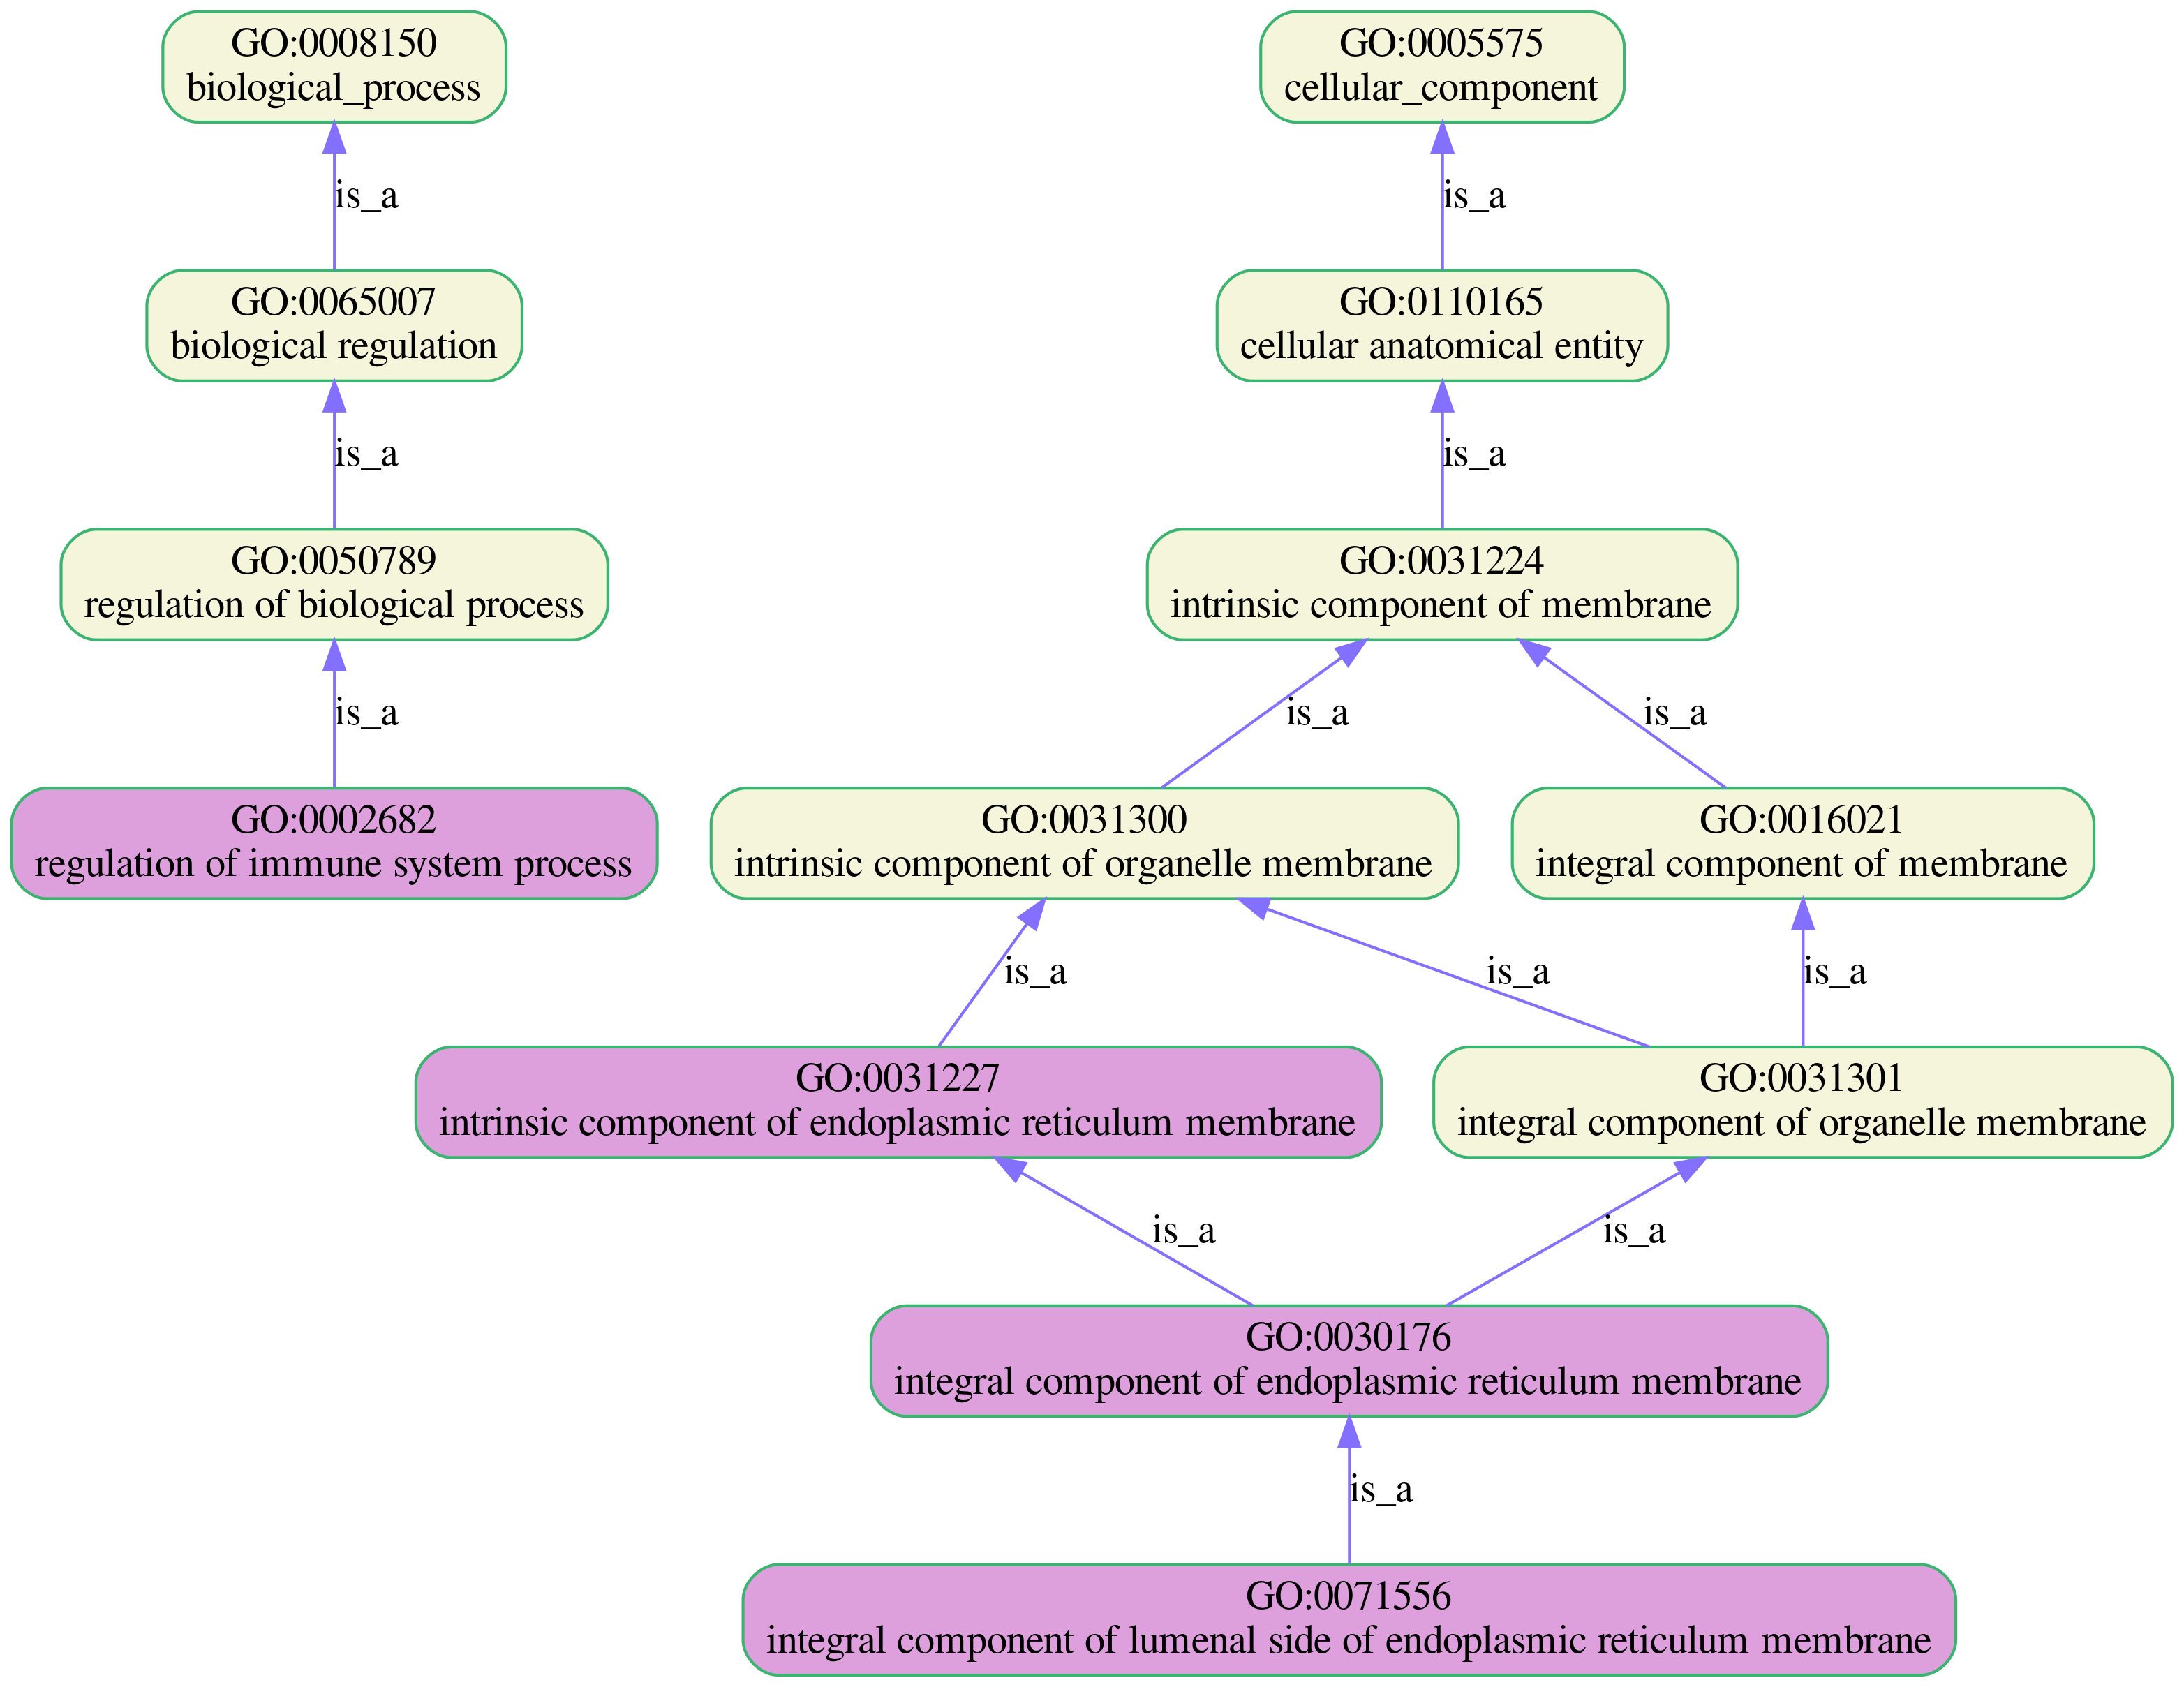
\includegraphics[width= 0.7\textwidth]{\plotspath{TCGA_OV_VST/GeneEnrichment/go_lineage_3_of_PCA_3.png}} \\
\begin{spacing}{0.6}
{\small Genes: \tiny \input{/home/ipoole/Documents/gitrepos/HgsocTromics/Plots/TCGA_OV_VST/GeneEnrichment/go_gene_set_3_of_PCA_3.txt}}
\end{spacing}
\vspace{0.5cm}
{\small Component PCA-3} \\
\end{center}
\caption{Lineage maps of enriched GO terms for component PCA-3. (Component PCA-2 produced no significant enrichment results)  }
\label{fig-PCA-3-3-go-lineage}

\end{figure}

Considering the biological significance of each of the 11 extracted metagenes, with reference to the GO enrichment results:
\begin{description}
%
\item[NMF-1]: there is mention of extra-cellular matrix (ECM) related terms, as in ICA-3 and NMF-1 below.   However, there are also terms relating to the regulation of angiogenesis.  It is known that tumours have a need for increased blood supply, and that expression level of factors promoting angigenesis are associated with aggresiveness of tumour growth \cite{Nishida2006}.  
We have already seen (section \ref{sec-subtype-classification}, \cite{Glass2015}) there is evidence for distinct subtypes of OC distinguished by angiogenesis related genes, and that these subtypes have been found to inform clinical outcome \cite{Glass2015}.  Thus, this component might contain useful prognostic value.
%
\item[NMF-2]: here we see enrichment of genes relating to the ribosomal subunit and the processes of RNA binding, implying perhaps a link with assembly of the ribosomal RNA-protein complex.   Ribosomes are known to have a role in carcinogenesis, by dysregulation the RNA $\rightarrow$ protein translation, or mutations in ribosomal subunits impacting on cellular metabolism \cite{Sulima2017}.
%
\item[NMF-3, ICA-1 and ICA-2]: no significant biological enrichment found.
%
\item[ICA-3]: this component relates to processes of multicellular / extracellular organisation, and the ECM.  It is therefore similar to NMF-1 above.
\item[ICA-4]: many processes are highlighted by the component.  These include processes relating to the ribosomal subunit (as NMF-2), additionally membrane proteins in the respiratory complex, mitochondrial and the NADH dehydrogenase complex.  Alsp processes of organonitrogen biosynthesis are also highlighted, purine nucleotide biosynthesis, RNA binding, proton membrane transport.
%
\item[ICA-5]: processes relating to regulation of immune response are enriched in this component, featuring genes from the major histocompatibility complex (MHC) group, in particular the HLA- genes, allowing the immune system to recognise self from non-self.  GO terms relating to the endoplasmic reticulum (ER) are also highlighted.  It may be that this component is mainly sensitive to the immunohistochemical signature of patients, and therefore not of clinical interest \footnote{This turns out to be an incorrect conclusion: note presence of gene CD38 and see the Discussion!}.
%
\item[PCA-1]: this is related to the cellular structures and processes of the ECM, that is the proteins such as collagens which mediate the three-dimensional organisation of cells in a tissues.  ECM molecular composition will vary substantially between tissue types, but is also known to play a part in many disease processes \cite{Theocharis2019}.  Thus, this metagene may simply reflect heterogeneity of tissues in the biopsied sample, or may have some deeper disease related significance.
%
\item[PCA-2]: no significant biological enrichment found.
%
\item[PCA-3]: this component has some similarity with ICA-5, in that it refers to regulation of immune processes (HLA- genes) and ER membrane.   However, chemotaxis (cell movement) is also highlighted.
\end{description}


\FloatBarrier

\subsection{Association of unsupervised gene expression patterns with patient survival is inconclusive}

Kaplan-Meier overall survival (OS) plots stratified by each metasample component are shown for the for the AOCS dataset in figure \ref{fig-kaplan-meier-os-TCGA-AOCS} and for the TCGA dataset in figure \ref{fig-kaplan-meier-os-TCGA-TCGA} (appendix).  Plots for progression free survival (PFS) on AOCS are also in the appendix, figure \ref{fig-kaplan-meier-pfs-TCGA-AOCS}.   All plots show 95\% confidence intervals and hazard ratio (HR) with associated p-value.

All of these results are summarised in figure \ref{fig-summary-survival-plots}, which brings together the three sets of results -- TCGA (OS), AOCS (OS) and AOCS (PFS) --  with respect to the 11 metasample components.  $\log_2{\mbox{HR}}$ is used in order that the \emph{sense} of the survival impact can be readily appreciated.    If a metasample component has a robust correlation with survival, then we expect the p-value for all three sets of results to show significance \emph{and} for the effects to have the same sense -- be in the same direction.  None of the 11 components pass this test.   

The component with the largest observed effect on survival is PCA-1, showing a reasonably consistent hazard ratio of around 1.3 ($2^{0.4}$) across the three experiments.  This has $p < 0.05$ in the larger TCGA dataset, but not in the smaller AOCS dataset.


\begin{figure}[htb!]
\begin{center}
\includegraphics[scale=0.4]{\plotspath{SurvivalAnalysis/multiple_kaplan_meier_os_TCGA_AOCS.pdf}} 
\caption{Kaplan-Meier plots for TCGA $\rightarrow$ AOCS for overall survival (OS).}
\label{fig-kaplan-meier-os-TCGA-AOCS}
\end{center}
\end{figure}


\begin{figure}[htb!]
\begin{center}
\includegraphics[scale=0.4]{\plotspath{/SurvivalAnalysis/survival_summary_barplots_NMF.pdf}} \\
\includegraphics[scale=0.4]{\plotspath{/SurvivalAnalysis/survival_summary_barplots_ICA.pdf}} \\
\includegraphics[scale=0.5]{\plotspath{/SurvivalAnalysis/survival_summary_barplots_PCA.pdf}}
\caption{Visual summary of survival analysis as applied to TCGA(OS), AOCS(OS) and AOCS(PFS).  Plots are divided by factorization method.  Bar heights show $\log_2(\mbox{HR})$ with p-value also shown.}
\label{fig-summary-survival-plots}
\end{center}
\end{figure}


\subsection{Metasamples correlate with some genomic features}

From the grid of scatter plots shown in figure \ref{fig-genomic-scatters} it can be seen there are some significant correlations at play.  These are summarised and analysed in the next section.


\begin{figure}[htb!]
\begin{center}
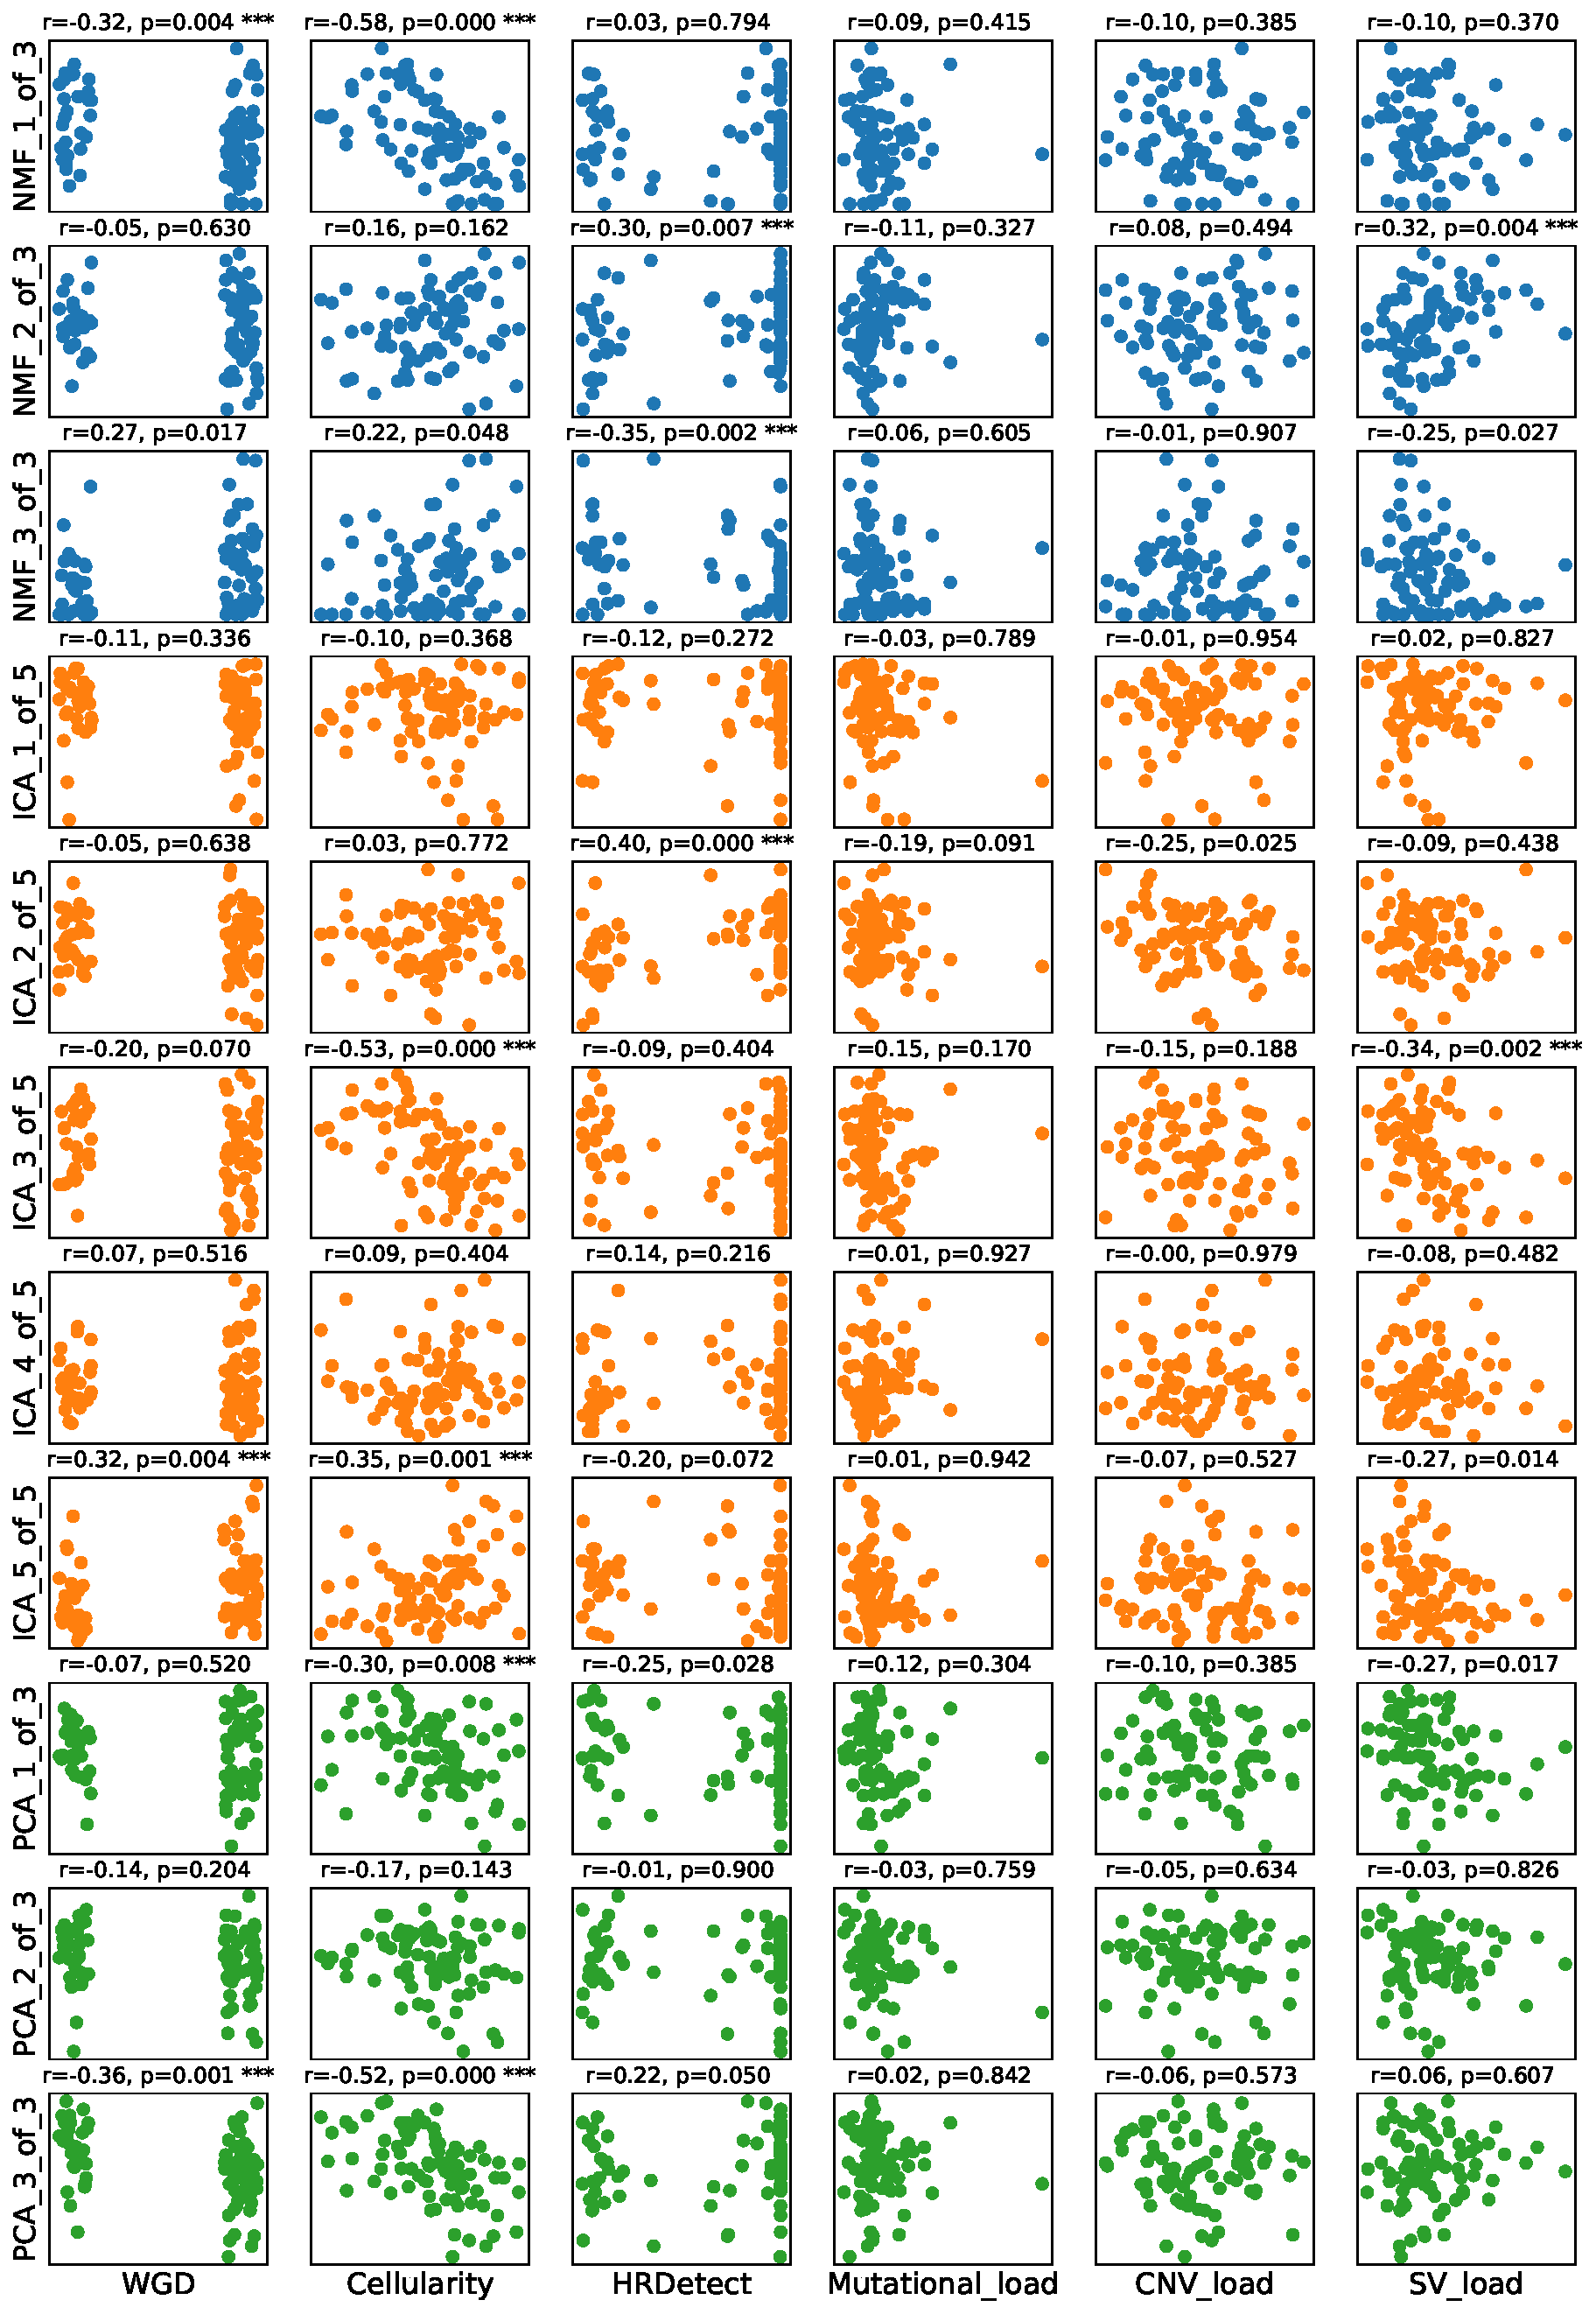
\includegraphics[scale=0.45]{\plotspath{BoxAndScatters/genomic_feature_scatters_TCGA_AOCS.pdf}} 
\caption{Grid of scatter plots to visualise the correlation between metasamples and genomic features.  In the case of WGD which has binary values (0, 1), jitter is applied for visual effect only.   Above each plot is shown a correlation coefficient $r$ and associated p-value, highlighted with '***' where $p < 0.01$.  In the case of WGD , the Point-Biserial correlation is used; for all others Pearson's $r$ is used.}
\label{fig-genomic-scatters}
\end{center}
\end{figure}


\FloatBarrier

\subsection{Integrative analysis of results}
\label{sec-integrative-analysis}

Table \ref{tab-integrative-analysis} summarises the key results of all the forgoing analysis.  
 
\begin{table}[htb!]
\begin{center}
\begingroup
\scriptsize
\renewcommand{\arraystretch}{1.4} % Default value: 1
\begin{tabular}{|l||c|c|c|c|c|c|c|p{4.5cm}|l|}
\hline
Metagene & S'val & WGD & Cell. & HRD & Mut.L. & CN.L. & SV.L. & Enriched GO terms & Similar to\\
\hline
%     & S & W & C & H % M & C & S & Enriched % Sim.
NMF-1 & . & Y-& Y-& . & . & . & . & ECM, Reg. angiogenesis & ICA-3, PCA-1 \\
NMF-2 & . & . & . & Y+& . & . & Y+& Ribo. subunit, RNA-binding & . \\
NMF-3 & . & . & . & Y-& . & . & . & . & . \\
\hline
ICA-1 & . & . & . & . & . & . & . & . & PCA-2 \\
ICA-2 & . & . & . & . & . & . & . & . & . \\
ICA-3 & . & . & Y-& . & . & . & Y-& ECM, multicellular/extracellular organisation & NMF-1, PCA-1 \\
ICA-4 & . & . & . & . & . & . & . & Ribo. subunit, Mitochondria, NADH dehydrogenase, purine nucleotide synthesis, RNA binding, Proton membrane transport & . \\
ICA-5 & . & Y+& Y+& . & . & . & . & ER, Immune response, MHC & PCA-3 \\
\hline
PCA-1 & ?+& . & Y-& . & . & . & . & Extra-cellular matrix / organisation, & NMF-1, ICA-3 \\
PCA-2 & . & . & . & . & . & . & . & . & ICA-1 \\
PCA-3 & . & Y-& Y-& . & . & . & . & ER, Immune response, MHC, chemotaxis & ICA-5 \\
\hline
\end{tabular}
\endgroup
\end{center}
\caption{For each metagenes a 'Y' indicates that a significant correlation was observed with: Survival, WGD, HRD, Mutational load,  CNV load and SV load;  '?' indicates a questionable link; +ve / -ve correlation is indicated.  The next column gives a terse summary of the GEA results.  The final column lists the metagenes which are apparently similar -- having a Jaccard similarity of $\geq 0.35$.}
\label{tab-integrative-analysis}
\end{table}
From this summary table we can make some interesting observations:
\begin{description}
\item[ECM relationship to Cellularity?]
NMF-1, ICA-3 and PCA-1 each have an ECM association and we have noted this could be related to tissue type heterogeneity.   These three components (one from each of the methods) are also observed to be correlated with Cellularity.  The sense (+/-) of the correlation is meaningful for NMF (not so for ICA or PCA) and we see that ECM and thence tissue heterogeneity is negatively correlated with cellularity. This seems reasonable, in that a low Cellularity implies that a greater proportion of surrounding non-tumour tissue is included in the sample, so increasing heterogeneity.   That these three components turn out to be similar by the Jaccard index is as would be expected given their functional similarity.
\item[No consistent link with survival.]
The only component showing even questionable correlation with patient survival is  PCA-1.  This is associated with ECM terms, which may simply be due to Cellularity.  
Component ICA-4 highlights the greatest number of biological processes -- indeed the GO lineage map \ref{fig-ICA-4-go-lineage} needed to be pruned to fit on a page.  And yet this component shows no correlation with any disease related factors, neither survival nor genomic features.  It may be that this component is simply picking up on the normal metabolic activity of the cells.
\item[Is HRD linked with ribosomal processing?]  HRD is correlated with NMF-2 and NMF-3.  The first of these is associated with the ribonucleoprotein complex while the second shows no biological enrichment.
\item[Technical batch effects?]
There are four components (NMF-3, ICA-2, ICA-4 and PCA-2) showing no enrichment of GO terms.  These components also show almost no correlation with disease related factors (the exception being NMF-3 linking with HRD).  With that exception aside, we could conclude that these components have little biological meaning, and are instead picking up technical effects.  I do not know how the TCGA dataset was assembled; perhaps there are multiple batches within the set?
\item[WGD and Cellularity have curious common influences.]
The three components NMF-1, ICA-5 and PCA-3 (one from each method) correlate with both WGD and Cellularity, and in the same sense. 
This might suggest simply that WGD and Cellularity are themselves positively correlated, but this is not so: $r=-0.14, p=0.201$ for Point-Biserial correlation (data not shown).  Neither is there any close similarity between the three components by Jaccard, although ICA-5 and PCA-3 are both linked to immune response and MHC.   Is there some curious non-linear interaction?
\item[Mutational load CNV load are not captured by these components.]  This is somewhat surprising, perhaps the link would emerge with more extracted components.
\end{description} 

\subsection{Matrix factorization discovers and effectively removes batch effects}


\begin{figure}[htb!]
\begin{center}
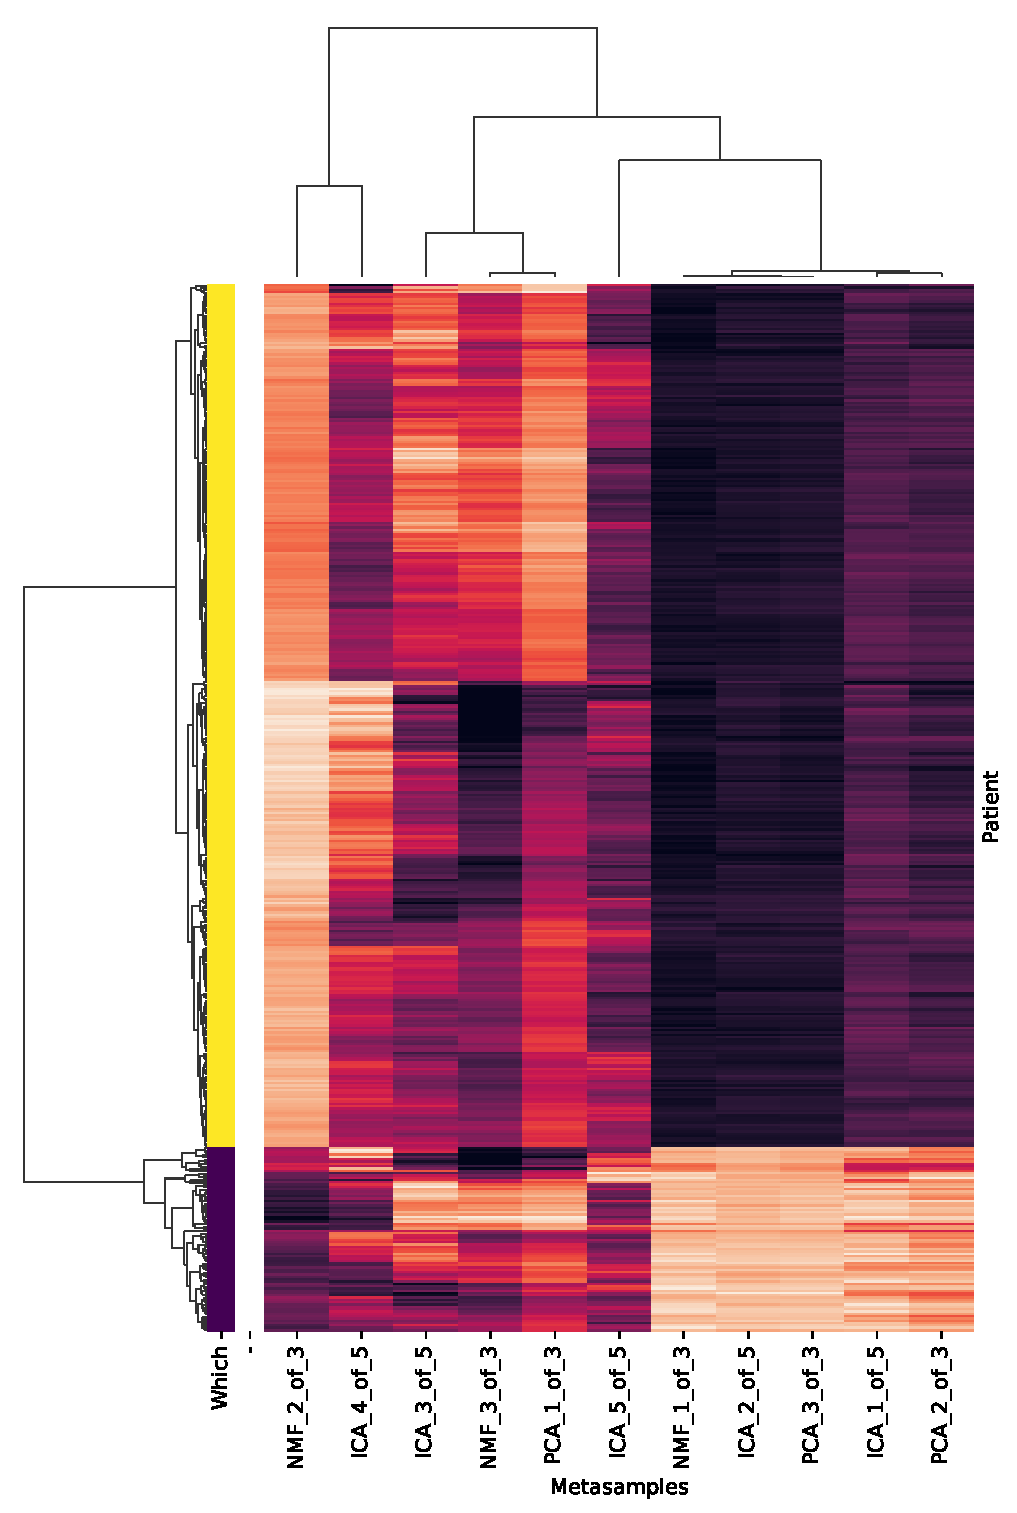
\includegraphics[scale=0.4,draft=false]{\plotspath{HeatMaps/clustered_heatmap_BOTH_BOTH.pdf}} 
\end{center}
\caption{Heatmap of the metasamples matrix for the combined AOCS + TCGA dataset.  The 'Which' field indicates the source dataset; purple: AOCS, yellow:TCGA.}
\label{fig-heatmap-BOTH}
\end{figure}


\begin{figure}[htb!]
\begin{center}
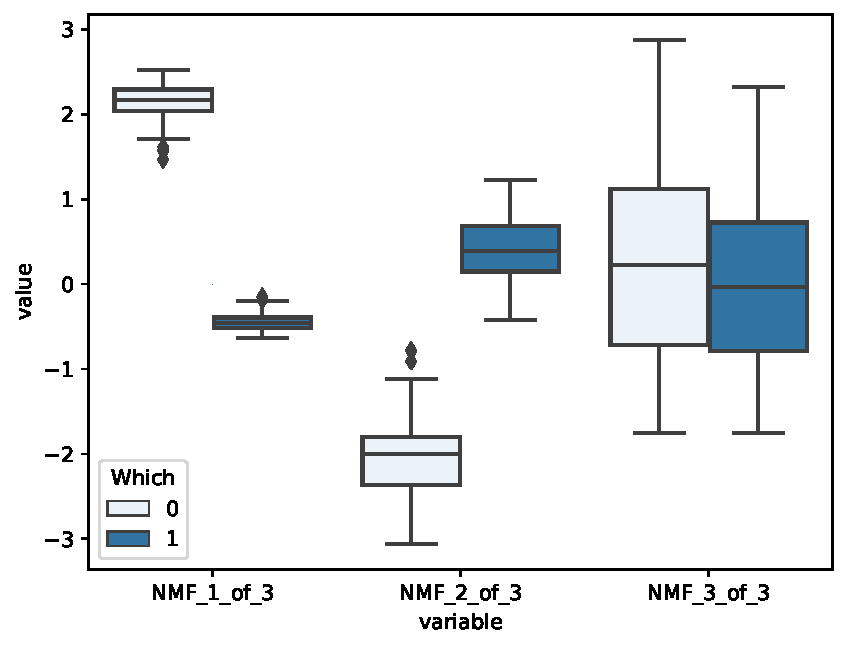
\includegraphics[scale=0.36]{\plotspath{BoxAndScatters/wgd_boxplot_NMF_BOTH_BOTH.pdf}}
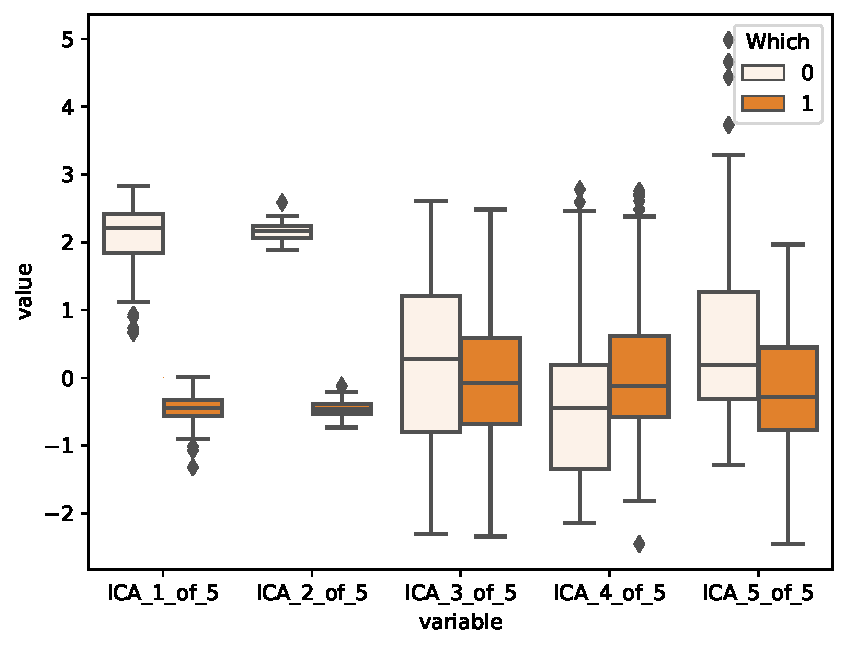
\includegraphics[scale=0.36]{\plotspath{BoxAndScatters/wgd_boxplot_ICA_BOTH_BOTH.pdf}}
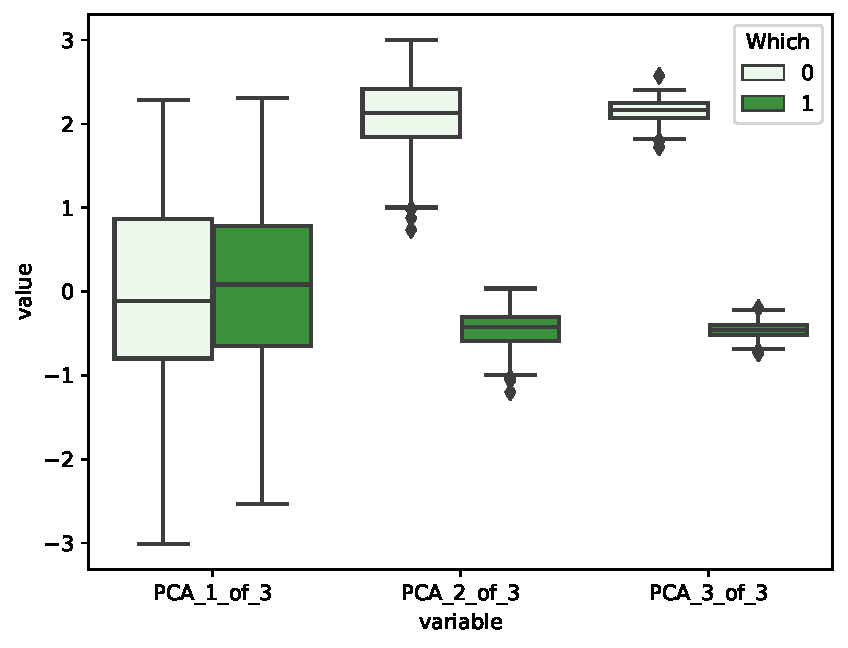
\includegraphics[scale=0.36]{\plotspath{BoxAndScatters/wgd_boxplot_PCA_BOTH_BOTH.pdf}}

\end{center}
\caption{Boxplots of metasamples from the combined AOCS + TCGA datasets, showing relationship between metasamples dataset origin; Which=0 or 1 for AOCS or TCGA respectively.}
\label{fig-boxplots-BOTH}
\end{figure}

Here are presented results of applying the three MF methods to the \emph{combined} AOCS and TCGA datasets. 
From the clustered heatmap of figure \ref{fig-heatmap-BOTH} it is clear that the five components clustered to the left are highly sensitive to (100\% predictive of) the batch, while in the other components batch is hardly discernable.  This is confirmed by the boxplots in figure \ref{fig-boxplots-BOTH}.   Within the larger TCGA dataset there is clear clustering into two groups with a roughly 5:6 ratio split.  Does this perhaps indicate that the TCGA set is collected from two separate sources?  Is the difference technical or are there substantially different cohorts of patients?

Table \ref{tab-integrative-analysis-BOTH} summarises observations on this combined dataset.  It can be seen that, with a few exceptions, a component is sensitive \emph{either} to Batch \emph{or} to some biological process, but seldom both.  This is a useful property.

\begin{table}[htb!]
\begin{center}
\begingroup
\scriptsize
\renewcommand{\arraystretch}{1.4} % Default value: 1
\begin{tabular}{|l||c|c|c|c|c|c|c|c|l|l|}
\hline
Metagene & Batch & WGD & Cell. & HRD & Mut.L. & CN.L. & SV.L. & Enrichment? \\
\hline
%     & B & W & C & H % M & C & S & Enrichment?
NMF-1 & Y & . & . & . & . & . & . &  Y \\
NMF-2 & Y & Y & Y & . & . &   & . &  Y \\
NMF-3 & . & Y & Y & . & . & . & . &  Y \\
\hline
ICA-1 & Y & . & . & . & . & . & . &  . \\
ICA-2 & Y & . & . & . & . & . & . &  . \\
ICA-3 & . & . & . & . & . &   & . &  Y \\
ICA-4 & . & Y & Y & . & . & . & . &  Y \\
ICA-5 & . & . & . & . & . & . & . &  Y \\
\hline
PCA-1 & . & Y & Y & . & . & . & . &  Y \\
PCA-2 & Y & . & . & . & . & . & . &  . \\
PCA-3 & Y & . & . & . & . & . & . &  . \\
\hline
\end{tabular}
\endgroup
\end{center}
\caption{In a similar format as table \ref{tab-integrative-analysis}, this summarises results of in respect of the \emph{combined AOCS and TCGA} datasets.  The key point here is that a known batch effect has been introduced, reflected in the 'Batch' column.  The `Enrichment' column simply indicates whether or not biological enrichment was found (the details have not been analysed).   Note that since these metagenes have been re-extracted from different data, they are distinct from those analysed in the previous section}
\label{tab-integrative-analysis-BOTH}
\end{table}

\clearpage

\section{Discussion}

Addressing each research questions in turn:

\subsubsection*{What underlying biological processes are at play in HGSOC as seen through the patterns of gene expression? }

Biological processes identified by GEA have been set out in section \ref{sec-gea}.   Processes relating to the ECM and extracellular organisation may reflect cell type heterogeneity -- perhaps within the tumour its self, or due to sampling of adjacent normal tissue.   Processes of negative regulation of angiogenesis could reflect tumour growth and therefore be of prognostic value.   

These observations are based on GEA on the GO only.  Possibly more insights could have been gained by GEA against KEGG\footnote{\href{https://www.genome.jp/kegg/pathway.html}{Kyoto Encyclopedia of Genes and Genomes}} Pathways. (This was begun but had to be dropped due to shortage of time).

\subsubsection*{How do the patterns of gene expression uncovered relate to genome level features, such as those marking genome instability?}

The integrative analysis set out in section \ref{sec-integrative-analysis} suggests that  Cellularity is correlated to the processes of the the ECM, reflecting heterogeneity of tissue type.   Of course, Cellularity is not really a biological characteristic -- it is a technical artefact of the tumour biopsy process, and so we might conclude that signatures relating to ECM might also be considered as technical artefacts.  We found that whole genome doubling (WGD) and Cellularity correlate together with three components even though they are not themselves directly correlated -- something which warrants further investigation.

Weak evidence of a link between homologous repair deficiency (HRD) and RNA-binding was found.   Being the site of protein synthesis, ribosomes will be associated with most of what goes on in a the cell.   One paper suggests a link : ``a comprehensive review of the literature reveals a role for conventional DNA repair proteins in ribosome biogenesis, and conversely, ribosome biogenesis proteins in DNA repair" \cite{Ogawa2018}.   Seek and ye shall find!

A note of caution: these results are based on testing $6 \times 11 = 66$ hypotheses at a significance level of $< 0.01$, so there will likely be at least one false discovery.  A significance level of 0.001 would have been more appropriate.

Expression signature correlations with mutational load and  CNV load have not been detected.  

\subsubsection*{Do MF methods yield factors which are predictive of patient survival?}

We found no convincing evidence of this, for an individual factor (metasample).  Some components were predictive in one or other of the two datasets, but not both, which is unconvincing.  The factor for which GEA indicated regulation of angiogenesis (NMF-1), and thence might have prognostic value, performed poorly in survival analysis.  So overall a negative result.

Is there a signal for survival to be found in these data?  We have noted that according to \cite{Zhu2020}, the single gene CD38 is highly predictive of survival in EOC.  Does this hold for the TCGA and AOCS datasets we are working with?  This is easy to check, running survival analysis stratified by a hand-crafted metagene, setting the CD38 element to 1, all others to 0.   This was applied as in section \ref{sec-survival-analysis} to TCGA (OS),  AOCS (OS) and AOCS (PFS) -- see figure \ref{fig-cd38 survival}.   The effects are in a consistent direction across the three tests, with high CD38 expression predicting favourable survival.  This is highly significant in the TCGA dataset and $p < 0.05 $ in the smaller AOCS.  So there is a signal, but it did not emerge unbidden from matrix factorization.  (CD38 is in fact highlighted by component ICA-5, see figure \ref{fig-ICA-5-5-go-lineage}, but must be diluted by other genes).

\begin{figure}
\begin{center}
\includegraphics[scale=0.5,draft=false]{\plotspath{SurvivalAnalysis/gene_specific_CD38_survival.pdf}}
\end{center}
\caption{Survival analysis plots stratified by above/below median expression of CD38 only.}
\label{fig-cd38 survival}
\end{figure}

Several other specific genes have been noted in section \ref{sec-review-of-gene-expression}; it would be interesting to test these also.


\subsubsection*{How should MF methods be applied to achieve robust results on datasets of limited size?}

One valuable lesson from this work is the importance of accounting for sampling error  when considering the stability of factorizations and thence the selection of factorization rank.    Sevaral authors comment on the variability of NMF and ICA factorization due to algorithm initialisation \cite{Kairov2017,Sompairac2019,WayGregory2019}, but most neglect sampling error which we have shown to be far more significant.   Cantini \etal\ \cite{Cantini2019a} mention bootstrapping, in reference to the BIODICA package (for ICA factorization), but it is unclear whether this is applied to the input data to model sampling error.  In the initial stages of this project, experiments were conducted with BIODICA on the AOCS dataset.   The package recommend ranks of 14, 19 or 30.  Yet we have seen that such high ranks on the small N=80 dataset leads to highly unstable factorizations when bootstrap modelling of sampling error is included.  Suspicion of this result lead to me roll my own implementation based on bootstrap resampling as described, resulting in much lower ranks (fewer metagenes) being selected than would otherwise be the case if only algorithmic randomness were considered.

\subsubsection*{Does MF detect and remove technical batch effects?}

Yes. We have been able to confirm the observations of \cite{Zhou2018a,Renard2016,Meng2016} that detection and removal of technical  batch effects naturally emerge from MF methods.  That is, the technical and biological variation largely (not completely) separate into different components.  This is a useful property, particularly as the growing availability of transcriptomics datasets from resources such as TCGA and GEO allows for the simultaneous analysis of dozens of distinct datasets with likely different technical provenance, for which hand crafted normalisation would be infeasible.

\subsubsection*{Which MF method is best suited to transcripomics analysis?}

The original technical focus of this dissertation was ICA and NMF since these are know to be able to disentangle variation in data with complex structure, not multivariate normally distributed.  PCA was added as a baseline dimensionality reduction method, just for comparison.   What would we have been missed if only PCA had been used?  Reviewing the integrative analysis of results in table \ref{tab-integrative-analysis} we see that all three methods picked up on WGD and cellularity.  PCA included the two components having the largest observed effect on overall survival.  NMF and ICA both showed sensitivity to SV load.  NMF further added sensitivity to HRD and identified genes relating to angiogenesis with possible pathological significance.

So it's a mixed picture.  Of course, had more components been selected from each method then likely more would have been found, but at the expense of robustness and thence false discovery, as we have discussed.   It seems we must concur with the conclusion of Way \etal \cite{WayGregory2019} that no one method excels, each brings individual value.   At least these three methods are simple and linear (unlike the VAE for example), and so can be used together easily.


\subsection{Further work}

This work has thrown up several possible lines of further study:
\begin{enumerate}
\item
{\bf Algorithm hyper-parameters}.  NMF and ICA algorithms have a number of hyper-parameters, only a few of which were explored in this work.  For example, NMF has parameters to encourage sparsity through L1 regularization.   This should result in many (most?) metagene elements reducing to zero, and might offer a more robust means of selecting candidate genes to feed into GEA -- replacing the current arbitrary 3 SD from the mean rule.
\item
{\bf Selecting components from several factorization ranks}.
In the current work, a single rank was selected for each method -- 3, 5 an 3 for NMF, ICA and PCA respectively.  Unlike PCA, components extracted by NMF and ICA  do not `nest' with rank; that is adding rank in general yields a new set of components.  Thus one might, for NMF and ICA, perform factorizations at $k=2,3,4,5$, say, yielding $2 \times 15 = 30$ potential components in total.  Jaccard similarity could be used to identify that subset of components which had the least overlap in detected genes.   In this way, a larger number of components could be obtained without use of high factorization ranks which we have seen to be unstable.  In fact this is similar to the approach of \cite{WayGregory2019} mentioned in section \ref{sec-comparative-dimensionality-studies}.  It will be important to take a principled approach to the setting of the FDR theshold when applying GEA, to account for the increased number of hypothesis being tested.
\item
{\bf Cross-dataset factorization stability}.  We went to considerable effort -- through bootstrap sampling and cluster analysis -- to select factorization ranks which we hoped would be robust and generalise well to other datasets.   A way to confirm this robustness would be to perform the factorization / clustering pipeline on \emph{both} datasets separately, yielding two sets of metagenes.  In a perfect world, these metagenes would pair up identically (in-so-far as the two datasets had identical technical characteristics, drawn from identical population of patients).  The Jaccard similarity heatmap could be used to verify this, and reject components which showed low cross-dataset similarity.  This proposal chimes to some extent with the use of Reciprocally Best Hit graphs in \cite{Cantini2019} reviewed in section \ref{sec-comparative-dimensionality-studies}.  
\item
{\bf Systematic comparison with published gene expression patterns}.  In analysing the meaning of each metagene above, some tentative links were made with the research literature, by informal searching.   A more systematic and ideally automated approach is required.  The \href{https://www.ncbi.nlm.nih.gov/geoprofiles}{Geo Profiles database} at NCBI, or the \href{https://www.ebi.ac.uk/gxa/home}{Expression Atlas} at EMBL-BI might be possible starting points.

\end{enumerate}

\clearpage

\section{Conclusions}

This work has investigated the application of unsupervised matrix factorization (MF) methods  -- specifically non-negative matrix factorization (NMF), independent component analysis (ICA) and principal component analysis (PCA) -- to gene expression analysis in the context of high grade serous ovarian cancer (HGSOC).  These methods aim to find metagenes which capture biologically or technically significant variation in the gene expression signal.  Metagenes were extracted from a N=374 patient dataset. Key findings are:
\begin{itemize}
\item
Biological processes relating to  extracellular matrix (ECM), ribosomal subunits, RNA binding, angiogenesis and immune response have been identified and may have significance to HGSOC.
\item
Metagenes have been found with possible correlation to genome level features of whole chomosome doubling, homologous repair deficiency and structural variant load.  However, these findings have marginal statistical significance given the small size (N=80) of the available dataset.
\item
A metagene predictive of patient survival did \emph{not} emerge from these unsupervised methods.
\item
However, expression of a single gene, CD38, identified from the literature, was confirmed to have substantial impact on patient survival.
\item
When applying MF methods, particularly to small datasets, it is important to consider the impact of sampling error when deciding the number of metagenes to extract.  Bootstrap resampling and cluster analysis is an effective approach.
\item
MF methods have been found effective in separating technical variation (batch effect) from biological variation.
\item
NMF, ICA and PCA each find mostly different metagenes. No clear evidence has been found to support one over the others.

\end{itemize}

\clearpage
\subsection*{Acknowledgements}
I am most grateful to Dr. Ailith Ewing for proposing this project and making available the datasets.  Ailith provided excellent, insightful supervision throughout and gave valuable feedback on an early draft of this dissertation.  I'd like to thank my employer, Canon Medical Research Europe Ltd., for allowing me the flexibility and study leave to undertake this MSc.  Thank you to my family for excusing me from cooking and washing up duties during the more stressful phases of MSc study and dissertation writing!

\small
\bibliography{OvarianCancer}
\bibliographystyle{ieeetr}
\normalsize

\newpage
\section{Appendices}
\subsection{Metagene clustering -- additional figures}
\def\S{0.3}
\begin{figure}[htb!]
\begin{center}
\includegraphics[scale=\S]{\plotspath{AOCS_Protein/FactorClustering/multiple_single_factors_scatter_AOCS_NMF_2_3_5_10_fixed.pdf}} \\
\includegraphics[scale=\S]{\plotspath{AOCS_Protein/FactorClustering/multiple_single_factors_scatter_AOCS_NMF_2_3_5_10_bootstrap.pdf}}\\
\caption{Clustering of metagenes from NMF facorizations on the AOCS dataset, comparing fixed and bootstrap sampling}
\label{fig-AOCS-nmf-fixed-vs-bootstrap}
\end{center}
\end{figure}


\begin{figure}[htb!]
\begin{center}
\includegraphics[scale=\S]{\plotspath{AOCS_Protein/FactorClustering/multiple_single_factors_scatter_AOCS_PCA_2_3_5_10_fixed.pdf}} \\
\includegraphics[scale=\S]{\plotspath{AOCS_Protein/FactorClustering/multiple_single_factors_scatter_AOCS_PCA_2_3_5_10_bootstrap.pdf}}\\
\caption{Clustering of metagenes from PCA facorizations on the AOCS dataset, comparing fixed and bootstrap sampling}
\label{fig-AOCS-pca-fixed-vs-bootstrap}
\end{center}
\end{figure}

\subsection{GEA -- additional plot}

\begin{sidewaysfigure}[htb!]
\begin{center}
\includegraphics[width=\textwidth]{\plotspath{TCGA_OV_VST/GeneEnrichment/go_lineage_4_of_ICA_5.png}} \\
\begin{spacing}{0.6}
{\small Genes: \tiny \input{/home/ipoole/Documents/gitrepos/HgsocTromics/Plots/TCGA_OV_VST/GeneEnrichment/go_gene_set_4_of_ICA_5.txt}}
\end{spacing}
\vspace{0.5cm}
\caption{Lineage maps of enriched GO terms for component ICA-4. For this component it was necessary to additionally filter the enriched terms -- see text.}
\label{fig-ICA-4-go-lineage}
\end{center}
\end{sidewaysfigure}

\FloatBarrier
\subsection{Survival analysis -- additional figures}

\begin{figure}[htb!]
\begin{center}
\includegraphics[scale=0.4]{\plotspath{SurvivalAnalysis/multiple_kaplan_meier_os_TCGA_TCGA.pdf}} 
\caption{Kaplan-Meier plots for each metasample component, stratified at the median value, for TCGA $\rightarrow$ TCGA for overall survival (OS) case.  Hazard ratio and p-value is shown for each case.  The final plot (bottom right) is unstratified overall survival}
\label{fig-kaplan-meier-os-TCGA-TCGA}
\end{center}
\end{figure}

\begin{figure}[htb!]
\begin{center}
\includegraphics[scale=0.4]{\plotspath{SurvivalAnalysis/multiple_kaplan_meier_pfs_TCGA_AOCS.pdf}} 
\caption{Kaplan-Meier plots for TCGA $\rightarrow$ TCGA for progression free survival (PFS).  }
\label{fig-kaplan-meier-pfs-TCGA-AOCS}
\end{center}
\end{figure}

\begin{figure}[htb!]
\begin{center}
\includegraphics[scale=0.5]{\plotspath{HeatMaps/clustered_heatmap_TCGA_AOCS.pdf}} 
\caption{Heatmap of the metasamples matrix for the AOCS dataset, computed from metagenes factorized from the TCGA dataset.   Several patient metadata variables are shown in columns to the left.}
\label{fig-heatmap-TCGA-AOCS}
\end{center}
\end{figure}

\FloatBarrier

\subsection{Batch effect investigation -- Additional figures}
\begin{figure}[htb!]
\begin{center}
\includegraphics[scale=\S]{\plotspath{BOTH_AOCS_TCGA/FactorClustering/multiple_single_factors_scatter_BOTH_NMF_2_3_5_10_bootstrap.pdf}} \\
\includegraphics[scale=\S]{\plotspath{BOTH_AOCS_TCGA/FactorClustering/multiple_single_factors_scatter_BOTH_ICA_2_3_5_10_bootstrap.pdf}} \\
\includegraphics[scale=\S]{\plotspath{BOTH_AOCS_TCGA/FactorClustering/multiple_single_factors_scatter_BOTH_PCA_2_3_5_10_bootstrap.pdf}} \\
\includegraphics[scale=0.55]{\plotspath{/BOTH_AOCS_TCGA/FactorClustering/silhouette_plots_BOTH_2_3_4_5_6_7_8_9_10_bootstrap.pdf}} 
\caption{Metagene clustering for all three methods applied to the combined N=80+374 AOCS + TCGA dataset with bootstrap sampling, over a range of factorization ranks.  The silhouette scores are also plotted (bottom).  }
\label{fig-BOTH-all-bootstrap}
\end{center}
\end{figure}


\begin{figure}[htb!]
\begin{center}
\includegraphics[scale=0.4]{\plotspath{BoxAndScatters/genomic_feature_scatters_BOTH_AOCS.pdf}} 
\caption{Grid of scatter plots to visualise the correlation between metasamples derived from the metagenes of the combined AOCS + TCGA datasets, and genomic features of the AOCS.}
\label{fig-genomic-scatters-BOTH-AOCS}
\end{center}
\end{figure}

\FloatBarrier

\subsection{Access to gene enrichment analysis table}
\label{tab-go-enrichment-results}

The table of GEA results is too large to conveniently include here.   If required it can be obtained from my github repository at \url{https://github.com/ipoole/HgsocTromics/blob/master/Results/combined_gea_fdr.tsv}.


\end{document}
